\documentclass[finnish,oneside]{book}
\usepackage[T1]{fontenc}
\usepackage[bottom=3cm]{geometry}
\usepackage{times}
\usepackage{moreverb}
\usepackage[sfdefault]{roboto}
\usepackage[utf8]{inputenc}
\usepackage[finnish]{babel}
%\usepackage{minted}
\usepackage[final]{pdfpages}
\usepackage{lscape}
\usepackage{array}%taulukkoon saa eri korkeuksiin soluun p,m,b
\usepackage{hyperref}
\hypersetup{
  colorlinks   = true, %Colours links instead of ugly boxes
  urlcolor     = blue, %Colour for external hyperlinks
  linkcolor    = black, %Colour of internal links
  citecolor   = black %Colour of citations
}


\setlength{\parindent}{0pt}          % Kappaleen alun sisennys (0pt, ts. ei sisennystä)
\setlength{\parskip}{3mm plus0.5mm minus0.5mm}
%\usepackage[utf8]{inputenc}		%imputenc-vaihtoehto 2, toimii paremmin ShareLaTeX-sivulla
%\usepackage[finnish]{babel}
\linespread{1.24} %riviväli 1.5
%\usepackage[T1]{fontenc}
%\usepackage[dvips]{graphicx}    %grafiikka paketti eps-kuvia varten
%\usepackage[pdftex]{graphicx}  %grafiikkapaketti jpg- yms. kuvia varten.
%\usepackage{psfrag}             %korvaa ps-fontteja
%\usepackage{dsfont}
\usepackage{amsfonts}           % AMS-paketteja
\usepackage{amsmath}
\usepackage{amssymb}
\usepackage{amsthm}
\usepackage{eurosym}            %euro-merkki \euro -komennolla
\pagestyle{plain}
\setlength\arraycolsep{2pt}
\usepackage{titleps}
\usepackage{fancyhdr}
\pagestyle{fancy}
\renewcommand{\chaptermark}[1]{\markboth{#1}{}}
\renewcommand{\sectionmark}[1]{\markright{#1}}
\fancyhf{}
\fancyhead[L]{\rightmark}
\fancyhead[R]{\leftmark}
\fancyfoot[C]{\thepage}
\fancyfoot[L]{LUMA-keskus Suomi}
\fancyfoot[R]{Arduino-paketti}
\renewcommand{\headrulewidth}{0.4pt}
\renewcommand{\footrulewidth}{0.4pt}
% \newpagestyle{fancy}{
%   \setheadrule{.4pt}% Header rule
%   \setfootrule{.4pt}% Footer rule
%   \sethead[\rightmark]% odd-left
%           []% odd-center
%           [\chaptertitle]% odd-right
%           {\chaptertitle}% even-left
%           {}% even-center
%           {\rightmark}% even-right
%   \setfoot[Arduino-paketti]% odd-left
%           [\thepage]% odd-center
%           [LUMA-keskus Suomi]% odd-right
%           {LUMA-keskus Suomi}% even-left
%           {\thepage}% even-center
%           {Arduino-paketti}% even-right
% }


% \newcommand{\veps}{\varepsilon}   %usein käytettyjen komentojen lyhenteitä
% \newcommand{\R}{\mathds{R}}
% \newcommand{\Z}{\mathds{Z}}
% \newcommand{\N}{\mathds{N}}        %lukujoukot
% \newcommand{\C}{\mathds{C}}
% \newcommand{\Q}{\mathds{Q}}
% \newcommand{\ekv}{\Leftrightarrow}  %ekvivalenssinuoli
% \newcommand{\imp}{\Rightarrow}       %implikaationuoli


% \newcommand{\viiva}{\mathop{\bigg/}}
% \newcommand{\sij}[3]{\viiva\limits_{\hspace*{-5mm}{#1}}^{\hspace*{5mm}{#2}}{#3}}
% % Suomalaiset sijoitusmerkit saadaan nyt komennolla \sij{a}{b}{F(x)}

% %\def\sij#1#2{\Big/_{\!\!\!#1}^{\,#2}\,}      % Suomalaiset sijoitusmerkit saadaan nyt komennolla
% %\def\Sij#1#2{\Bigg/_{\!\!\!\!\!\!#1}^{#2}}   % \sij^{yläraja}_{alaraja} tai \Sij^{yläraja}_{alaraja}

% \newenvironment{todistus}
% {\noindent{\it Todistus. }}{\hfill $\Box$\par\vspace{2.5mm}}  %todistus saadaan nyt \begin{todistus} \end{todistus} -komennolla

% \theoremstyle{plain}
% \newtheorem{lause}{Lause}[section]      %lauseiden yms. numerointi on päälukujen mukaan esim. Lause 2.1
% %\newtheorem{lause}{Lause}[subsection]   %lauseiden yms. numerointi on alalukujen mukaan esim. Lause 2.1.1
% \newtheorem{lemma}[lause]{Lemma}
% \newtheorem{propositio}[lause]{Propositio}    %ja toimii juoksevana
%                                         %näissä kaikissa joissa keskellä [lause]
% \newtheorem{seuraus}[lause]{Seuraus}        %perässä on lyhenteet, joilla saadaan
%                                         %aloitus- ja lopetusmerkit
% \theoremstyle{definition}
% \newtheorem{määritelmä}[lause]{Määritelmä}
% \newtheorem{konjektuuri}[lause]{Konjektuuri}
% \newtheorem{esimerkki}[lause]{Esimerkki}

% \theoremstyle{remark}
% \newtheorem{huomautus}[lause]{Huomautus}

% \numberwithin{equation}{section}        % numeroi yhtälöt kappaleittain. Jos vaihdat section tilalle subsection,
%                                         % niin numerointi alakappaleittain

% %\usepackage{makeidx}                    % nämä rivit mahdollistavat hakemiston luomisen
% %\makeindex                              % Jos sana halutaan hakemistoon, laitetaan sen perään komento\index{sana}
%                                         % Hakemistoa käytetään ainakin kirjoissa ja silloin jos työ on hyvin laaja
% %\addto\captionsfinnish{%
%   %\renewcommand{\figurename}{Figure}%
% %	\renewcommand{\refname}{Lähteet}%
% %}
\addto\captionsfinnish{\renewcommand{\refname}{Lähteet}}

\usepackage{tikz} %kuvatyökalupaketti

\usepackage{fancybox} %laatikkokehykset tekstiin
\newenvironment{fminipage}% luo minipage-ympäristön käytettäväksi komennolla \begin{fminipage}{2in} ... \end{fminipage}
{\begin{Sbox}\begin{minipage}}%
{\end{minipage}\end{Sbox}\fbox{\TheSbox}}
\usepackage{xcolor} %väripaketti, tunnistaa esim. blue!20
\usepackage[most]{tcolorbox}

\makeatletter
\def\@makechapterhead#1{%
  {\parindent \z@ \raggedright \normalfont
    \ifnum \c@secnumdepth >\m@ne
        \huge\bfseries \thechapter.\ % <-- Chapter # (without "Chapter")
    \fi
    \interlinepenalty\@M
    #1\par\nobreak% <------------------ Chapter title
    \vskip 20\p@% <------------------ Space between chapter title and first paragraph
  }}
\makeatother

% %%%%%% Arduino coding settings
 %%%%%%%%%%%%%%%%%%%%%%%%%%%%%%%%%%%%%%%%%%%%%%%%%%%%%%%%%%%%%%%%%%%%%%%%%%%%%%%% 
%%% ~ Arduino Language - Arduino IDE Colors ~                                  %%%
%%%                                                                            %%%
%%% Kyle Rocha-Brownell | 10/2/2017 | No Licence                               %%%
%%% -------------------------------------------------------------------------- %%%
%%%                                                                            %%%
%%% Place this file in your working directory (next to the latex file you're   %%%
%%% working on).  To add it to your project, place:                            %%%
%%%    \input{arduinoLanguage.tex}                                             %%%
%%% somewhere before \begin{document} in your latex file.                      %%%
%%%                                                                            %%%
%%% In your document, place your arduino code between:                         %%%
%%%   \begin{lstlisting}[language=Arduino]                                     %%%
%%% and:                                                                       %%%
%%%   \end{lstlisting}                                                         %%%
%%%                                                                            %%%
%%% Or create your own style to add non-built-in functions and variables.      %%%
%%%                                                                            %%%
 %%%%%%%%%%%%%%%%%%%%%%%%%%%%%%%%%%%%%%%%%%%%%%%%%%%%%%%%%%%%%%%%%%%%%%%%%%%%%%%% 

\usepackage{color}
\usepackage{listings}    
\usepackage{courier}
\usepackage[utf8]{inputenc}
\usepackage{accsupp}


%%% Define Custom IDE Colors %%%
\definecolor{arduinoGreen}    {rgb} {0.17, 0.43, 0.01}
\definecolor{arduinoGrey}     {rgb} {0.47, 0.47, 0.33}
\definecolor{arduinoOrange}   {rgb} {0.8 , 0.4 , 0   }
\definecolor{arduinoBlue}     {rgb} {0.01, 0.61, 0.98}
\definecolor{arduinoDarkBlue} {rgb} {0.0 , 0.2 , 0.5 }

%%% Define Arduino Language %%%
\lstdefinelanguage{Arduino}{
  language=C++, % begin with default C++ settings 
%
%
  %%% Keyword Color Group 1 %%%  (called KEYWORD3 by arduino)
  keywordstyle=\color{arduinoGreen},   
  deletekeywords={  % remove all arduino keywords that might be in c++
                break, case, override, final, continue, default, do, else, for, 
                if, return, goto, switch, throw, try, while, setup, loop, export, 
                not, or, and, xor, include, define, elif, else, error, if, ifdef, 
                ifndef, pragma, warning,
                HIGH, LOW, INPUT, INPUT_PULLUP, OUTPUT, DEC, BIN, HEX, OCT, PI, 
                HALF_PI, TWO_PI, LSBFIRST, MSBFIRST, CHANGE, FALLING, RISING, 
                DEFAULT, EXTERNAL, INTERNAL, INTERNAL1V1, INTERNAL2V56, LED_BUILTIN, 
                LED_BUILTIN_RX, LED_BUILTIN_TX, DIGITAL_MESSAGE, FIRMATA_STRING, 
                ANALOG_MESSAGE, REPORT_DIGITAL, REPORT_ANALOG, SET_PIN_MODE, 
                SYSTEM_RESET, SYSEX_START, auto, int8_t, int16_t, int32_t, int64_t, 
                uint8_t, uint16_t, uint32_t, uint64_t, char16_t, char32_t, operator, 
                enum, delete, bool, boolean, byte, char, const, false, float, double, 
                null, NULL, int, long, new, private, protected, public, short, 
                signed, static, volatile, String, void, true, unsigned, word, array, 
                sizeof, dynamic_cast, typedef, const_cast, struct, static_cast, union, 
                friend, extern, class, reinterpret_cast, register, explicit, inline, 
                _Bool, complex, _Complex, _Imaginary, atomic_bool, atomic_char, 
                atomic_schar, atomic_uchar, atomic_short, atomic_ushort, atomic_int, 
                atomic_uint, atomic_long, atomic_ulong, atomic_llong, atomic_ullong, 
                virtual, PROGMEM,
                Serial, Serial1, Serial2, Serial3, SerialUSB, Keyboard, Mouse,
                abs, acos, asin, atan, atan2, ceil, constrain, cos, degrees, exp, 
                floor, log, map, max, min, radians, random, randomSeed, round, sin, 
                sq, sqrt, tan, pow, bitRead, bitWrite, bitSet, bitClear, bit, 
                highByte, lowByte, analogReference, analogRead, 
                analogReadResolution, analogWrite, analogWriteResolution, 
                attachInterrupt, detachInterrupt, digitalPinToInterrupt, delay, 
                delayMicroseconds, digitalWrite, digitalRead, interrupts, millis, 
                micros, noInterrupts, noTone, pinMode, pulseIn, pulseInLong, shiftIn, 
                shiftOut, tone, yield, Stream, begin, end, peek, read, print, 
                println, available, availableForWrite, flush, setTimeout, find, 
                findUntil, parseInt, parseFloat, readBytes, readBytesUntil, readString, 
                readStringUntil, trim, toUpperCase, toLowerCase, charAt, compareTo, 
                concat, endsWith, startsWith, equals, equalsIgnoreCase, getBytes, 
                indexOf, lastIndexOf, length, replace, setCharAt, substring, 
                toCharArray, toInt, press, release, releaseAll, accept, click, move, 
                isPressed, isAlphaNumeric, isAlpha, isAscii, isWhitespace, isControl, 
                isDigit, isGraph, isLowerCase, isPrintable, isPunct, isSpace, 
                isUpperCase, isHexadecimalDigit, 
                }, 
  morekeywords={   % add arduino structures to group 1
                break, case, override, final, continue, default, do, else, for, 
                if, return, goto, switch, throw, try, while, setup, loop, export, 
                not, or, and, xor, include, define, elif, else, error, if, ifdef, 
                ifndef, pragma, warning,
                }, 
% 
%
  %%% Keyword Color Group 2 %%%  (called LITERAL1 by arduino)
  keywordstyle=[2]\color{arduinoBlue},   
  keywords=[2]{   % add variables and dataTypes as 2nd group  
                HIGH, LOW, INPUT, INPUT_PULLUP, OUTPUT, DEC, BIN, HEX, OCT, PI, 
                HALF_PI, TWO_PI, LSBFIRST, MSBFIRST, CHANGE, FALLING, RISING, 
                DEFAULT, EXTERNAL, INTERNAL, INTERNAL1V1, INTERNAL2V56, LED_BUILTIN, 
                LED_BUILTIN_RX, LED_BUILTIN_TX, DIGITAL_MESSAGE, FIRMATA_STRING, 
                ANALOG_MESSAGE, REPORT_DIGITAL, REPORT_ANALOG, SET_PIN_MODE, 
                SYSTEM_RESET, SYSEX_START, auto, int8_t, int16_t, int32_t, int64_t, 
                uint8_t, uint16_t, uint32_t, uint64_t, char16_t, char32_t, operator, 
                enum, delete, bool, boolean, byte, char, const, false, float, double, 
                null, NULL, int, long, new, private, protected, public, short, 
                signed, static, volatile, String, void, true, unsigned, word, array, 
                sizeof, dynamic_cast, typedef, const_cast, struct, static_cast, union, 
                friend, extern, class, reinterpret_cast, register, explicit, inline, 
                _Bool, complex, _Complex, _Imaginary, atomic_bool, atomic_char, 
                atomic_schar, atomic_uchar, atomic_short, atomic_ushort, atomic_int, 
                atomic_uint, atomic_long, atomic_ulong, atomic_llong, atomic_ullong, 
                virtual, PROGMEM,
                },  
% 
%
  %%% Keyword Color Group 3 %%%  (called KEYWORD1 by arduino)
  keywordstyle=[3]\bfseries\color{arduinoOrange},
  keywords=[3]{  % add built-in functions as a 3rd group
                Serial, Serial1, Serial2, Serial3, SerialUSB, Keyboard, Mouse,
                },      
%
%
  %%% Keyword Color Group 4 %%%  (called KEYWORD2 by arduino)
  keywordstyle=[4]\color{arduinoOrange},
  keywords=[4]{  % add more built-in functions as a 4th group
                abs, acos, asin, atan, atan2, ceil, constrain, cos, degrees, exp, 
                floor, log, map, max, min, radians, random, randomSeed, round, sin, 
                sq, sqrt, tan, pow, bitRead, bitWrite, bitSet, bitClear, bit, 
                highByte, lowByte, analogReference, analogRead, 
                analogReadResolution, analogWrite, analogWriteResolution, 
                attachInterrupt, detachInterrupt, digitalPinToInterrupt, delay, 
                delayMicroseconds, digitalWrite, digitalRead, interrupts, millis, 
                micros, noInterrupts, noTone, pinMode, pulseIn, pulseInLong, shiftIn, 
                shiftOut, tone, yield, Stream, begin, end, peek, read, print, 
                println, available, availableForWrite, flush, setTimeout, find, 
                findUntil, parseInt, parseFloat, readBytes, readBytesUntil, readString, 
                readStringUntil, trim, toUpperCase, toLowerCase, charAt, compareTo, 
                concat, endsWith, startsWith, equals, equalsIgnoreCase, getBytes, 
                indexOf, lastIndexOf, length, replace, setCharAt, substring, 
                toCharArray, toInt, press, release, releaseAll, accept, click, move, 
                isPressed, isAlphaNumeric, isAlpha, isAscii, isWhitespace, isControl, 
                isDigit, isGraph, isLowerCase, isPrintable, isPunct, isSpace, 
                isUpperCase, isHexadecimalDigit, 
                },      
%
%
  %%% Set Other Colors %%%
  stringstyle=\color{arduinoDarkBlue},    
  commentstyle=\color{arduinoGrey},    
%          
%   
  %%%% Line Numbering %%%%
  numbers=left,                    
  numbersep=5pt,                   
  numberstyle=\color{arduinoGrey},    
  %stepnumber=2,                      % show every 2 line numbers
%
%
  %%%% Code Box Style %%%%
  breaklines=true,                    % wordwrapping
  tabsize=2,         
  basicstyle=\ttfamily  
} 
\usepackage{accsupp}
\newcommand{\noncopynumber}[1]{%
    \BeginAccSupp{method=escape,ActualText={}}%
    #1%
    \EndAccSupp{}%
}

\lstset {%
    numbers = left,%
    numberstyle=\noncopynumber,
    frame=single,
    language=Arduino,
    showstringspaces=false
}
%%%%%%%%%%
\usepackage{comment}
\usepackage{tcolorbox}
% Make ourselves a new conditional
% Use \HideSolutionstrue to "activate" it
\newif\ifHideSolutions
% Make a solution environment
\generalcomment{solution}{%
  \begingroup
  \ifHideSolutions%
  % if \HideSolutionstrue is called, then we remove the contents
  \def\ProcessCutFile{}\fi%
}{%
  \ifHideSolutions%
    % aand,now (also when it's not called), we make a box
    % and then we \input the \CommentCutFile.
    \phantom{\input{\CommentCutFile}}
    %\setbox1=\vbox{\input{\CommentCutFile}}%
    % Get the height from \ht1 and use \vskip to make appropriate space
    %\vskip\ht1
  \fi
\endgroup%
}
%%%%%%%%%%%%%%%%
\usepackage{circuitikz}
\usepackage{pgfplots}
\usetikzlibrary{shadings,backgrounds,scopes}
\usetikzlibrary{calc,intersections,positioning}

%%https://tex.stackexchange.com/questions/493239/alignment-of-dip-chips-in-circuitikz
%%https://lpn-doc-sphinx-primer.readthedocs.io/en/stable/extensions/tikz/circuitikz.html#id11

\definecolor{hopea}{HTML}{C0C0C0}
\tikzset{% Environment Config
    font=\small,
    open socket/.style = {
        circle,
        fill = lightgray,
        draw = lightgray,
        inner sep = 1pt
    },
    filled socket/.style = {
        circle,
        fill = black,
        draw = lightgray,
        inner sep = 1pt
    },
    strip/.style = {
        opacity = 0.1,
        line cap = round,
        line join = round,
        line width = 6pt
    },
    wire/.style = {
        decorate,
        decoration = {
            random steps,
            amplitude = 2pt,
            segment length = 0.2in
        },
        line cap = round,
        line join = round,
        line width = 2pt
    },
    european resistors
}

% You can create an smart objet like Henri Menke in this post:
% --> http://www.texample.net/tikz/examples/4-bit-counter/
% Variables: 1: Position 2: Lines.
\def\BREADBOARD(#1)#2{%
    \begin{scope}[shift={(#1)}]
        \foreach \y [evaluate = \y as \line using int(abs(\y))]
                 in {-1,-2,-3,...,-#2}{%% draw breadboard sections

            % draw bus and breadboard grid sockets
            \foreach \lab/\x in {
                    l-/-8, lg/-7,       % power strips on left side
                    A/-5, B/-4, C/-3, D/-2, E/-1, % left side
                    F/1, G/2, H/3, I/4, J/5,     % right side
                    r+/7, rg/8         % power strips on right side
            } {
                \coordinate [open socket] (\lab\line) at (\x, \y);
            }

            % draw row connectivity for board proper
            \begin{scope} [% these paths should not interfere with anything else
                on background layer
            ]
                \draw [strip,gray]
                    (A\line.west) -- (E\line.east)
                    (F\line.west) -- (J\line.east);
            \end{scope}

            % draw line numbers off to the left
            \node [left of = l-\line,text=gray] {\line};
            \node [right of = rg\line,text=gray] {\line};
        }

        % draw bus connection lines
        \begin{scope} [% these paths should not interfere with anything else
            on background layer
        ]
            \draw [strip,red]  (l-1.north) -- (l-#2.south);
            \draw [strip,black] (lg1.north) -- (lg#2.south);
        
            \draw [strip,red]  (r+1.north) -- (r+#2.south);
            \draw [strip,black] (rg1.north) -- (rg#2.south);
        \end{scope}

        % label breadboard columns (top/bottom)
        \foreach \lab/\x in {
                A/-5, B/-4, C/-3, D/-2, E/-1, % left side
                F/1, G/2, H/3, I/4, J/5      % right side
        } {
            \node [above of = \lab1] {\lab};
            \node [below of = \lab#2] {\lab};
        }

        % label buses (top)
        \node [above of=l-1,red] {\Large{${+}$}};
        \node [above of=lg1,black] {\Large{${-}$}};
        \node [above of=r+1,red] {\Large{${+}$}};
        \node [above of=rg1,black] {\Large{${-}$}};
        % label buses (bottom)
        \node [below of=l-#2,red] {\Large{${+}$}};
        \node [below of=lg#2,black] {\Large{${-}$}};
        \node [below of=r+#2,red] {\Large{${+}$}};
        \node [below of=rg#2,black] {\Large{${-}$}};
    \end{scope}
}

%%%%%%%%%% DEFINE ARDUINO %%%%%%%%%%%%%%%%%%
\definecolor{rgreen}{HTML}{228b22}
\tikzset{%
myarduino/.pic={
\coordinate (A) at (0,0);
\filldraw[rgreen] (A)--++(4,0)--++(2,-1)--++(8,0)--++(2,1)++(4,0)-|++(0,40)--++(-20,0)-|++(0,-40)--cycle;
\filldraw[very thick,black](1,39) rectangle (4,42);
\filldraw[very thick,gray!40](9,38) rectangle (12.5,43);

\foreach \x/\t in {9/Vin,10/GND1,11/GND2,12/5V,13/3.3V,14/RESET,15/IOREF}{
\node (Ar\t) at (1,2*\x) [fill=black,draw]{};
\node[color=white] at (1,2*\x) [right=0.5]{$\mathbf{\t}$};}

\foreach \x/\n in {1/A5,2/A4,3/A3,4/A2,5/A1,6/A0}{
\node (Ar\n) at (1,2*\x) [fill,draw]{};
\node[color=white] at (1,2*\x) [right=3mm]{$\mathbf{\n}$};}

\foreach \x/\n in {1/0,2/1,3/2,4/3,5/4,6/5,7/6,8/7,10/8,11/9,12/10,13/11,14/12,15/13,16/GND3,17/AREF,18/SDA,19/SCL}{
\node (Ar\n) at (18,2*\x) [fill,draw,minimum width=3mm,minimum height=3mm]{};
\node[color=white] at (18,2*\x) [left=0.5]{$\mathbf{\n}$};}
}}
%%%%%%%%%%%%%%%%%%%%%%%%%%%%%%%%%

\usepackage[
    type={CC},
    modifier={by-nc-sa},
    version={3.0},
]{doclicense}
%%%%%%%%%%%%%%%%

%%%%%%%%%%%%%%%%%

%Uncomment below to hide solutions
% Kommentoituna näyttää ratkaisut
% Poista kommenttimerkki, niin et näe ratkaisuja

%\HideSolutionstrue


\title{Arduino-paketti yläkouluun ja lukioon}
\author{}
\date{}


\begin{document}

\begin{titlepage}
%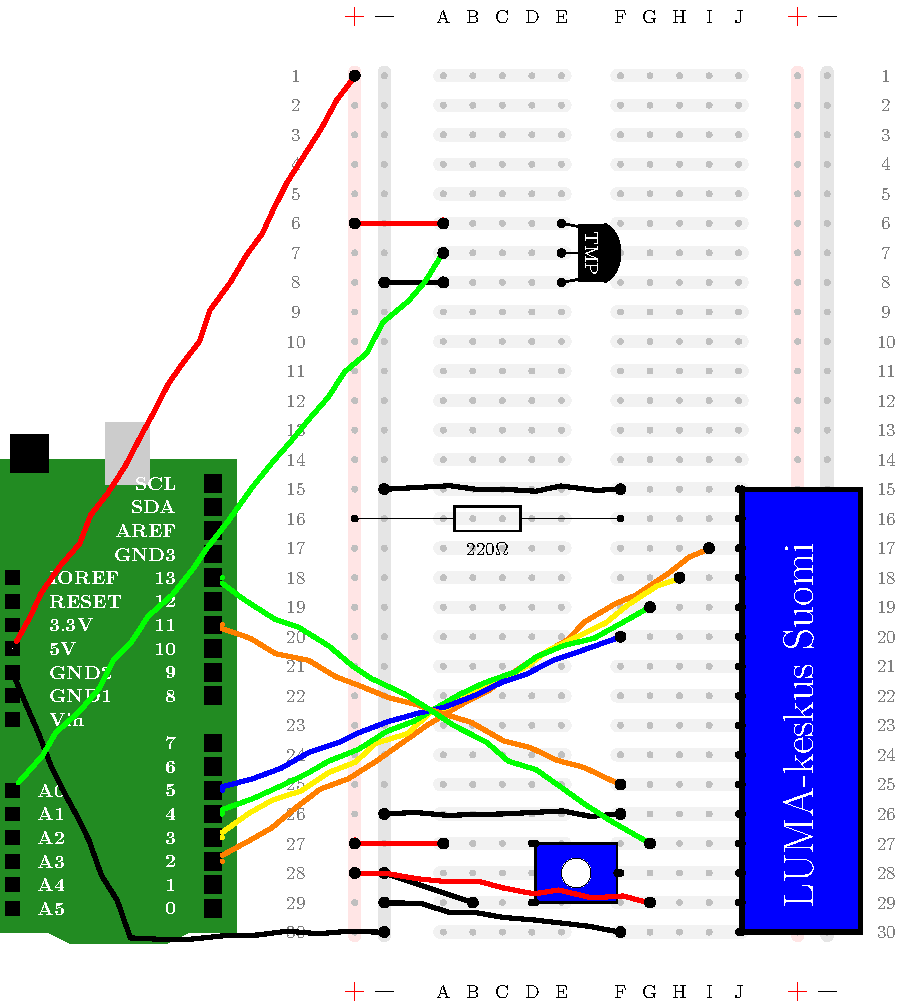
\includegraphics[width=\paperwidth,height=\paperheight,%
%keepaspectratio]{kuvat/kansikuva.pdf}%
\begin{tikzpicture}[remember picture,overlay]
%\shadedraw[inner color=orange!70!white,outer color=yellow!30!white] (current page.center) circle (5cm) node {\Huge \textbf{Title of the project}};
\path (current page.south) +(-8,+5) coordinate (B);
\node[above right,draw=none,fill=none] at (B) {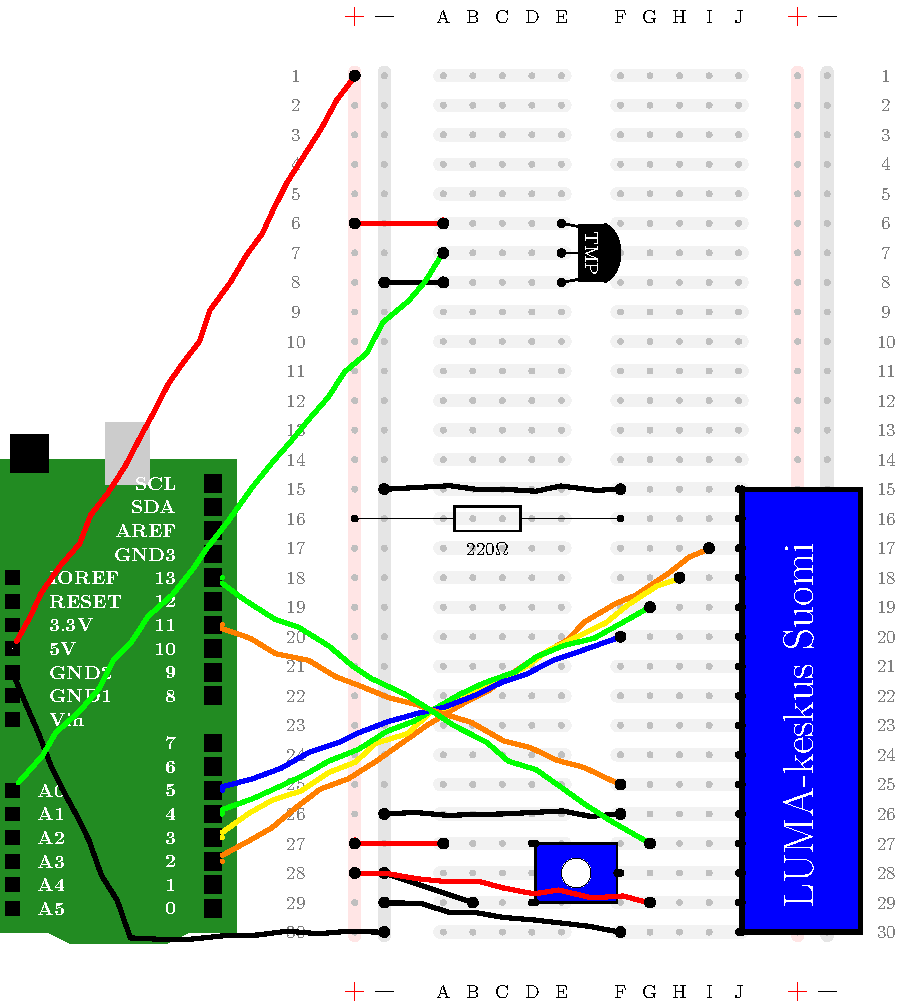
\includegraphics[bb=0 0 0 0]{kuvat/kansikuva.pdf}};
\path (current page.north) +(0,-5) coordinate (A);
\node at (A) {\Huge{Arduino-paketti yläkouluun ja lukioon}};
\end{tikzpicture}

\end{titlepage}

\pagestyle{plain}
%%%%%%%%%%%% Käyttölisenssi
\begin{tcolorbox}[title = Käyttölisenssi]
Tämä materiaali rakentaa ja muokkaa Arduinon Projects Book:n ohjeita, jotka on lisensoitu Nimeä-EiKaupallinen-JaaSamoin 3.0 Ei sovitettu (CC BY-NC-SA 3.0) (Attribution-NonCommercial-ShareAlike 3.0 Unported (CC BY-NC-SA 3.0)). 


Alkuperäinen tekijä: \url{arduino.cc} 

Muokkaajat: Heli Virtanen ja Pekka Muotka

Materiaalin testaajat ja kommentoijat: Janne Rantanen ja Ilkka Palonen

Alkuperäisen materiaalin lisensin mukaisesti, myös tämän materiaalipaketin materiaaleja voi käyttää lisenssin CC BY-NC-SA 3.0 mukaisesti. 

\doclicenseThis

\tcblower
Lisäksi ideoita ja inspiraatiota materiaalin pohjaksi ovat antaneet LUMA-keskus Saimaan sekä Aalto-yliopiston Arduino-materiaalit. 

\url{https://act.aalto.fi/fi/aalto-yliopisto-junior/materiaalit}

Kiitokset myös tiedekasvatuskurssin opiskelijoille L. Sihvonen ja M. Moilanen. 

%\url{https://www.lut.fi/yhteistyo-ja-palvelut/luma-keskus}

\end{tcolorbox}

\begin{tcolorbox}[title=Taustaa]
Tämä materiaali on tehty LUMA-keskus Suomen sekä kehittäjäkoulujen kanssa yhteistyössä lukuvuoden 2021-2022 aikana. 

Materiaalia kehitettiin koulujen toiveiden pohjalta ja kehittämisyhteistyö jatkuu edelleen. 

\tcblower
Paketista julkaistaan kesän 2022 LUMA-päivien yhteydessä versio, jota tullan myöhemmin täydentämään. LUMA-keskus Suomen sivuilta löytyy koko materiaali käyttövalmiina PDF-tiedostona ja lisäksi siellä on linkki kehitysversioon. Tämä versio on tarkoitettu erityisesti sähköisesti käytettäväksi ja täytettäväksi, mutta toimii myös paperiversiona.
\end{tcolorbox}

\begin{center}

\includegraphics[width=0.3\textwidth]{kuvat/luma_flower-multicolored_text-black-vertical-fi.png}
\end{center}

\pagestyle{fancy}
\tableofcontents

\clearpage


%
\chapter{Esittely}

\section{Arduino}

”Open Source Electronics Prototyping Platform”

Arduino/Genuino on avoimeen laitteistoon ja ohjelmistoon perustuva mikrokontrolleri-elektroniikka-alusta ja ohjelmointiympäristö. Arduinon avulla toteutetussa laitteessa on kaksi kokonaisuutta: Arduinoon liitetty ulkoinen kytkentä ja Arduinoon syötetty ohjelma.

Arduinokortin INPUT-napoihin voi liittää erilaisia antureita, säätimiä tai kytkimiä, jotka ohjaavat OUTPUT- napoihin kytkettyjä ledejä, releitä, servoja tai moottoreita. Laitteen toiminnot määritetään laitteeseen syötetyllä ohjelmalla. Arduino-ympäristö tarjoaa helpon ja halvan keinon opetella elektroniikkaa ja ohjelmointia nykyaikaisella tavalla.

Arduino on hyvin avoin konsepti ja erilaisia *duino-tuotteita myydään nettikauppojen välityksellä huokeaan hintaan. Euroopassa ”aidot” Arduino-tuotteet myydään Genuino-nimen alla. Projektin kotisivu on osoitteessa www.arduino.cc.


\newpage
\subsection*{Arduinon osat}

\begin{figure}[h!]
    \begin{tikzpicture}[remember picture]
\node (fig1) at (0,0)
       {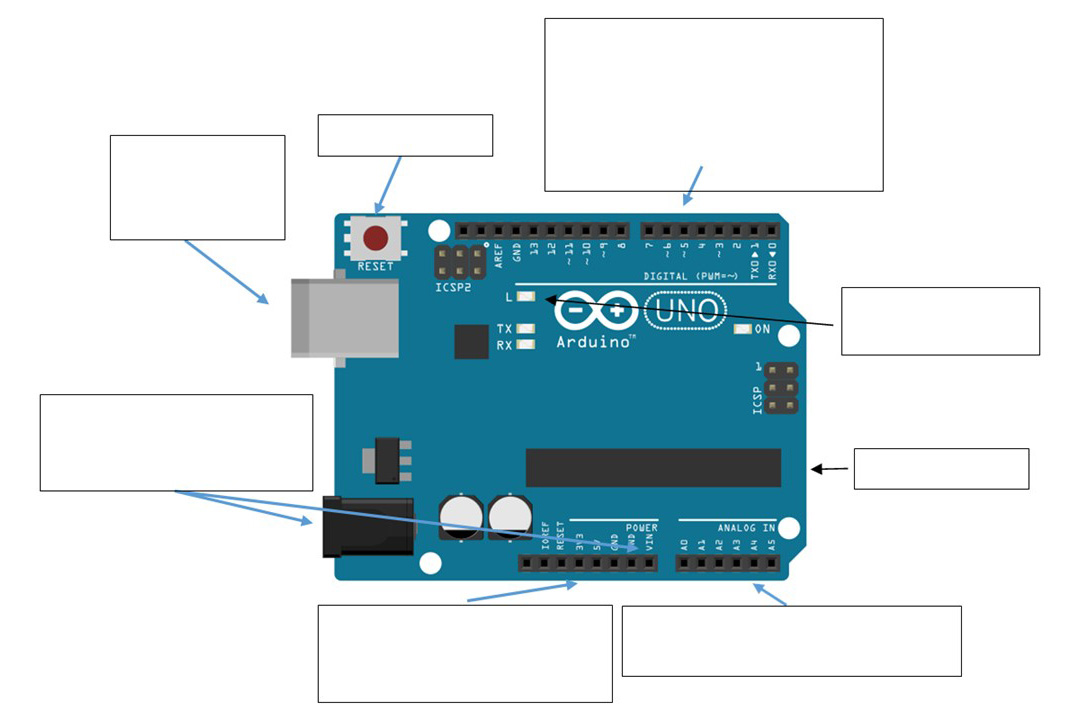
\includegraphics[scale=0.55]{kuvat/arduino.jpg}};
\end{tikzpicture}
\begin{tikzpicture}[remember picture, overlay]
       \node [align=left,] at (10.5,9.55) {\small 14 digitaalista kytkentäpinniä\\\small (voidaan ohjelmallisesti määrittää\\\small  joko INPUT-tai OUTPUT-pinneiksi)\\\small LOW = 0 = 0 V \\\small  HIGH = 1 = +5 V };
      \node [align=left] at (2.6,4.65) {\small Ulkoinen virransyöttö\\\small (6...15 V, 2,1 mm virtaliitin\\\small tai Vin -pinni)};
      \node [align=left] at (3,8.4) {USB-liitin\\ koodin \\ja virran
    syöttö };
      \node [align=left] at (5.95,9.15) {Reset-nappula};
      \node [align=left] at (13.8,6.45) {Pinniin 13 kytketty\\ledi};
      \node [align=left] at (13.8,4.3) {Mikrokontrolleri};
      \node [align=left] at (6.9,1.6) {\small Virtaliitäntä kytkentöjä varten,\\\small 5 V, GND (0 V eli maa)};
      \node [align=left] at (11.65,1.75) {\small 6 analogista kytkentäpinniä A0-A5\\\small lukevat jännitettä 0--5 V};
      

\end{tikzpicture}
    \caption{Arduino Unon osat}
    \label{fig:arduino_uno}
\end{figure}

%Arduinon osat ja niiden kuvaustekstit


\newpage
\subsection*{Koekytkentälevy}
Koekytkentälevy Kuva:\ref{fig:koekytkentalevy} (engl. Breadboard) on alusta, jolle voi koota kytkennän tarvitsematta juottaa komponentteja kiinni. Laitteet toteutetaan sijoittamalla komponentit koekytkentälevylle, jolloin samassa rivissä olevat komponenttien pinnit ovat yhteydessä toisiinsa. Ulkoiset liitokset Arduinoon ja muihin komponentteihin tehdään hyppylangoilla

Arduino/Genuino Starter Kit on aloittelevalle harrastajalle sopiva sarja, jossa Arduinokortin, komponenttien ja kattavan ohjekirjan lisäksi saa rakentelualustan, jossa samalle alustalle on asennettu Arduino Uno ja koekytkentälevy. Hieman halvemmalla alkuun pääsee hankkimalla pelkän Arduinokortin ja koekytkentälevyn. Tällöin muut komponentit täytyy kuitenkin hankkia erikseen.

Tutkimustöiden kytkentäkuvat on piirretty toteutettavaksi Starter Kitillä.



%koekytkentälevy
\begin{figure}[h!]
    \centering
    \begin{tikzpicture}[remember picture]
\node (fig1) at (0,0)
       {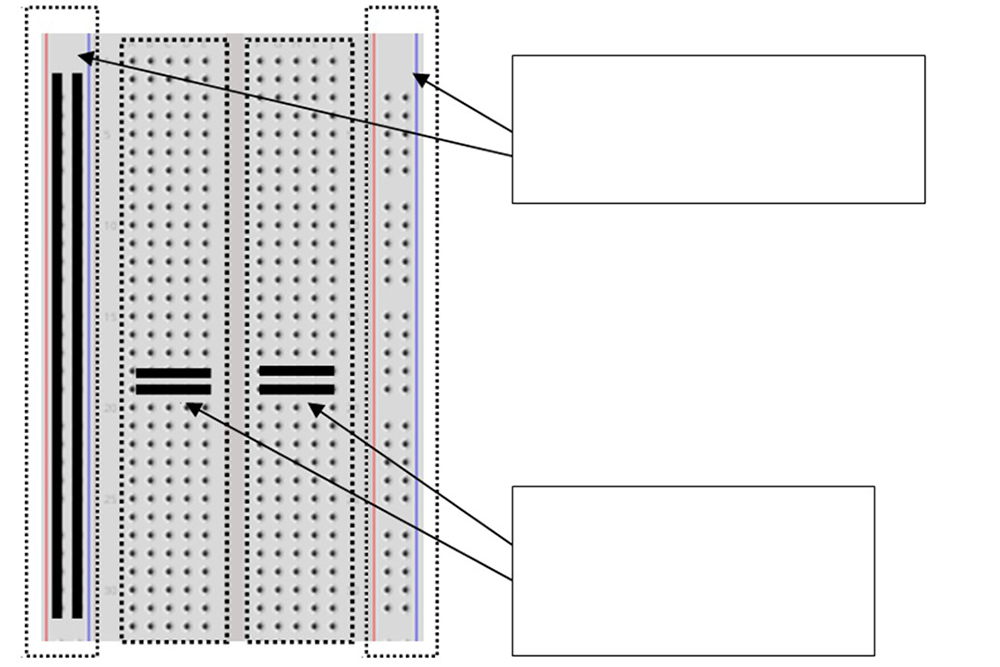
\includegraphics[scale=0.40]{kuvat/koekytkentalevy.jpg}};
\end{tikzpicture}
\begin{tikzpicture}[remember picture, overlay]
       \node [align=left,] at (-4.5,1.5) {Vaakarivi samaa\\ johdinta. Ura katkaisee johtimen.\\ Tähän kohtaan\\varsinainen kytkentä};
       \node [align=left,] at (-4.6,7.7) {Pystyrivi samaa johdinta.\\Tähän kytketään yleensä\\virransyöttö +5 V tai 0 v (GND) };
\end{tikzpicture}
    \caption{Koekytkentälevy, rivit ja sarakkeet levyllä. }
    \label{fig:koekytkentalevy}
\end{figure}
\newpage

\subsection*{Ohjelmointiympäristöt}

Lataa Arduinon ohjelmointiympäristö osoitteesta https://www.arduino.cc/en/Main/Software. Ohjelma on ilmainen ja voit valita nappulan ”Just download”. Jos haluat tukea ohjelman kehittäjiä, niin voit valita summan ja nappulan ”Contribute \& Download”. Sivulta löytyy Windows-, Mac- ja Linux-versiot.

Windows-versiota asennettaessa asennusohjelma antaa mahdollisuuden asentaa automaattisesti myös USB-ajurin. Ajuri kannattaa asentaa, koska ilman sitä tietokone ei tunnista Arduinokorttia.



\begin{center}
\begin{fminipage}{10cm}
\textbf{Ohjelman käyttö:}
\begin{enumerate}
    \item Avaa Arduino-ohjelma koneelle 
    \item Kytke Arduino-kortti USB-johdolla koneelle
    \item Tarkista Tools/Työkalut-valikosta Board/Kortti (Arduino Uno) ja Serial Port/Portti (yleensä COM3 tai suurempi)
    \item Ohjelma ”Sketch” ladataan Arduinolle vasemman yläkulman nuolella merkitystä nappulasta

\end{enumerate}
\end{fminipage}
\end{center}

Seikkaperäiset ohjeet ovat sivulla https://www.arduino.cc/en/Guide/Windows. Ohjeet löytyvät myös editoriohjelman Apua-toiminnosta.
\begin{center}
\begin{fminipage}{10cm}
    Ohjelmoinnin tärkein apusivusto on Arduinon oma opas osoitteessa https://www.arduino.cc/en/Reference/HomePage.
\end{fminipage}
\end{center}


\begin{figure}[h!]
    \centering
        \begin{tikzpicture}[remember picture]
\node (fig1) at (0,0)
       {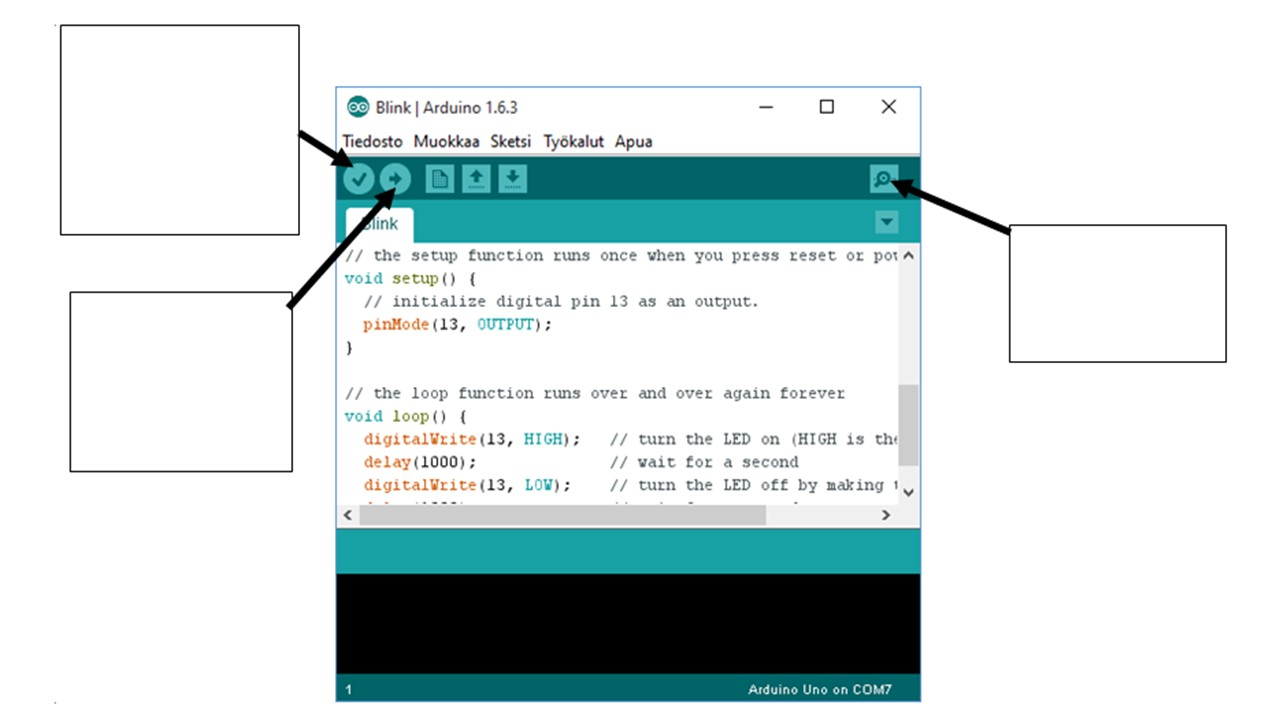
\includegraphics[scale=0.45]{kuvat/ohjelmointiymparisto.jpg}};
\end{tikzpicture}
\begin{tikzpicture}[remember picture, overlay]
       \node [align=left,] at (-5.4,7.7) {\textit{Verify/Tarkista}\\Ohjelma\\tarkistaa\\mutta ei ladata\\Arduinolle };
       \node [align=left,] at (-5.4,4.7) {\textit{Upload/Lataa}\\Ohjelma\\ladataan\\Arduinolle };
       \node [align=left,] at (5.85,5.7) {Avaa sarjaportin\\monitorointi-\\ikkunaan };
\end{tikzpicture}
    \caption{Arduinon ohjelmointiympäristö ja keskeiset hallinnointi painikkeet. }
    \label{fig:ohjelmointiymparisto}
\end{figure}

% \begin{figure}[h!]
%     %\centering
%     \begin{tikzpicture}[remember picture]
%     \node at (0,0) {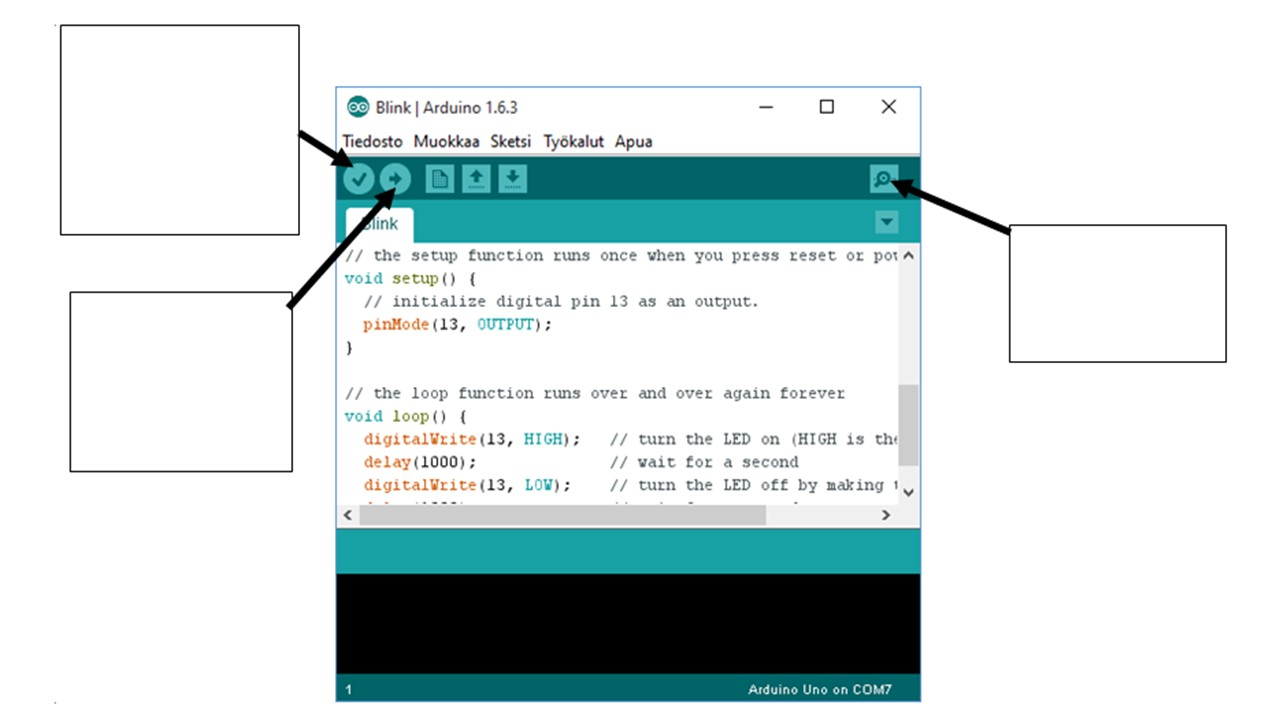
\includegraphics[scale=0.4]{kuvat/ohjelmointiymparisto.jpg}};
%     \end{tikzpicture}
%     \begin{tikzpicture}[overlay,remember picture]
    
%     \end{tikzpicture}
%     \caption{Arduinon ohjelmointiympäristö ja keskeiset hallinnointi painikkeet. }
%     \label{fig:ohjelmointiymparisto}
% \end{figure}
%%%input{kappaleet/BLINK}
%\section{Virtapiiri}
Virtapiiri on virtalähteiden, johtimien ja sähkölaitteiden muodostama sähkövirran kulkureitti. Kun virtapiiri on suljettu sen läpi kulkee sähkövirta.

\subsection*{Jännite}
Sähköinen jännite on kahden pisteen välinen sähköinen potentiaaliero. Jännitteen yksikkö on voltti, jonka symboli on V.
\subsection*{Sähkövirta}
Sähkövirta on sähkövarausten liikettä. Sähkövirta on suure. Sähkövirran yksikkö on ampeeri, joka symboli on A. Yksi ampeeri on yhden coulombin (C) suuruisen varauksen kulku johteen poikkipinnan läpi yhden sekunnin (s) aikana. 1 A = 1 C/s.

\subsection*{Resistanssi}
Resistanssi eli sähköinen vastus on suure, jonka tunnus on R. Resistanssi kuvaa johtimen tai muun sähköisen piiriosan kykyä vastustaa sähkövirtaa. Resistanssin mittayksikkö SI-järjestelmässä on ohmi, jonka tunnus on $\Omega$. Piirinosan resistanssi on yksi ohmi virtapiirissä, missä kahden pisteen välinen jännite on 1 voltti ja sähkövirta on yhden ampeerin.
($\Omega$ = V/A).
\subsection*{Teho}
Teho on suure, jonka tunnus on P. Teholla kuvataan tehdyn työn tai käytetyn energian määrää aikayksikössä. Tehon yksikkö on watti, jonka tunnus on W. Sähköinen teho on sähkövirran voimakkuuden  ja jännitteen tulo.
\subsection*{Tasavirta}
Tasavirta kulkee virtapiirissä koko ajan samansuuntaisesti. Sähkövirran voimakkuutta ilmaistaan voltteina. Akut ja paristot tuottavat tasavirtaa.

\subsection*{Vaihtovirta}
Vaihtovirta on sähkövirtaa, jonka suunta vaihtelee. Sähkövirran voimakkuutta ilmaistaan voltteina, sähkövirran suunnan muutostaajuutta kuvataan hertseillä. Suomessa kotitalouksissa käytettävä verkkovirta on sinimuotoista vaihtovirtaa, jonka vaihejännitteen tehollisarvo on nimellisesti 230 volttia ja taajuus 50 hertsiä.

\begin{tcolorbox}[colback=blue!10,colbacktitle=purple!90,title=\section*{Suureet}]

\begin{tabular}{ l{2.5cm}  c{1.5cm} c{2cm} c{1.5cm} r{3cm}   }
\textbf{ Mitattava suure}    &   \textbf{Suureen tunnus}    &   \textbf{Yksikön nimi}  & \textbf{Yksikön tunnus} & \textbf{Laskukaava}  \\
% \hline

sähkövirta  &   \textit{I}   &    ampeeri    &    A  &  $\displaystyle I=\frac{U}{R} $ \\
jännite &    \textit{U}  &	voltti  &	V   &	$\displaystyle U=R \cdot I $    \\
resistanssi & 	\textit{R }  &	ohmi    &  $\Omega$   &	$\displaystyle  R=\frac{U}{I}  $  \\
teho    &   \textit{P}   &	watti   & 	W   &	$P=U\cdot I$     \\
energia &	\textit{E}    &	joule   &	  J &	 $E=P\cdot t^*$  
\end{tabular}

*$t$ = aika

\end{tcolorbox}

\subsection*{Esimerkkejä}
\subsubsection*{Esimerkki 1: Sopiva vastus LED-valon kanssa}

Arduino Unoa käytetään virtalähteenä. Virtapiiriin kytketään yksi led-valo. Jotta led-valo toimisi toivotusti tulee ledin kanssa sarjaan kytkeä
sarjavastus, joka rajoittaa ledin läpi kulkevan sähkövirran noin 10-20 milliampeeriin (mA). Laske ja valitse sopiva vastus virtapiiriin.

Hehkuvan led-valon napojen välillä vaikuttaa ns. kynnysjännite, noin 1,5 V. Arduino Unon digitaalisessa pinnissä on 5
voltin jännite. Vastuksen napojen välinen jännite on siis (5 - 1,5) V = 3,5 V. Kun jännite ja sähkövirta
tiedetään, voidaan sopivan vastuksen resistanssin arvo laskea:

\begin{align*}
    R = \frac{U}{I} = \frac{3{,}5\text{V}}{0{,}02\text{A}} = 175\Omega
\end{align*}

\textbf{Ratkaisu:} Vastukseksi valitaan lähin vastus, 220 $\Omega$. 

\section{Ylesimittarin käyttö}
\subsection*{Vastuksen mittaaminen}
Ohje kuinka yleismittarilla mitataan vastuksen resistanssi.

\chapter{Koekytkentälevyn käyttö}

\section{Rinnankytkentä}
Kahden kaksijalkaisen komponentin rinnankytkentä saadaan aikaan laittamalla molempien komponenttien toinen jalka yhdelle riville ja toiset jalat jollekin muulle riville:


\begin{minipage}{0.75\textwidth}
\begin{center}
Koekytkentälevyllä
\end{center}
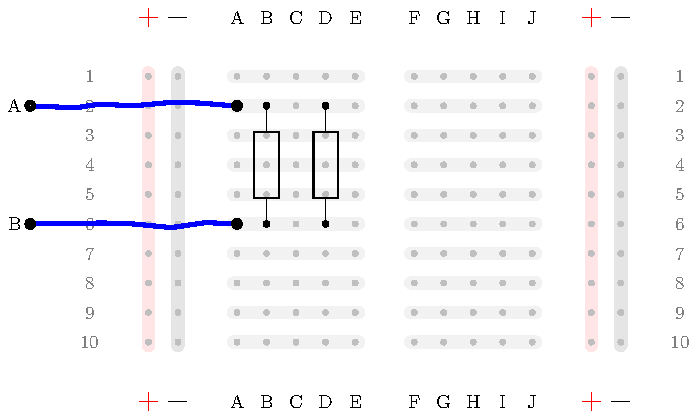
\includegraphics[width=0.8\textwidth]{kuvat/kuva1.pdf}
\end{minipage}%
\begin{minipage}{0.25\textwidth}
\begin{center}
Piirikaavio
\end{center}
\begin{tikzpicture}[scale=0.8]
%\draw (0,0) to[R] (0,5);
%\draw (3,0) to[R] (3,5);
\draw (0,0) node[anchor=east] {B} to[short, o-] (1,0) to[R,*-*] (1,2) -- (3,2) to[R] (3,0) -- (1,0) (1,2) to[short, -o] (0,2) node[anchor=east]{A};
\end{tikzpicture}
\end{minipage}
\begin{tcolorbox}[colback=yellow!10, title={Testaa taitosi!},colbacktitle=orange]
Piirrä toinen kaksijalkainen komponentti jo piirretyn komponentin rinnalle. Piirrä myös pisteet A ja B kuvaan.

\begin{tikzpicture}[scale=0.45]
\BREADBOARD (0,0) {10};
\draw (C3) to[R,*-*] (C7);
\unless\ifHideSolutions
\draw (E3) to[R,*-*] (E7);
\draw[blue,wire] (A3) to[short,*-o] ++(-7,0) node[left,black] {A};
\draw[blue,wire] (A7) to[short,*-o] ++(-7,0) node[left,black] {B};
\fi

\end{tikzpicture}\\
\begin{solution}
Kuvassa on esitetty yksi esimerkki, mutta myös muita vaihtoehtoja on olemassa.
\end{solution}
\end{tcolorbox}

%\clearpage
\section{Sarjaankytkentä}
Kahden kaksijalkaisen komponentin sarjankytkentä saadaan aikaan laittamalla molempien komponenttien toinen jalka yhdelle riville ja toiset jalat kahdelle muulle riville: 

\begin{minipage}{0.8\textwidth}
\begin{center}
Koekytkentälevyllä
\end{center}
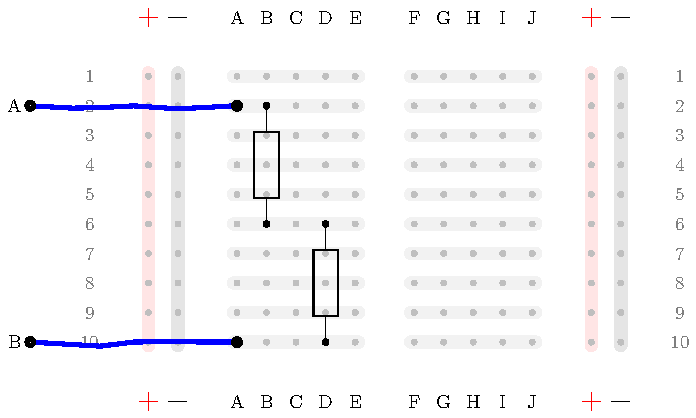
\includegraphics[width=0.9\textwidth]{kuvat/kuva2.pdf}
\end{minipage}
\begin{minipage}{0.2\textwidth}
Piirikaavio\\
\begin{tikzpicture}
%\draw (0,0) to[R] (0,5);
%\draw (3,0) to[R] (3,5);
\draw (0,0.5) node[anchor=east] {B} to[short, o-] (0,1) to[R] (0,3)--(0,3.5) to[R] (0,5.5) to[short,-o] (0,6) node[anchor=west]{A};
\end{tikzpicture}
\end{minipage}


\begin{tcolorbox}[colback=yellow!10, title={Testaa taitosi!},colbacktitle=orange]
Piirrä toinen kaksijalkainen komponentti jo piirretyn komponentin kanssa sarjaan. Piirrä myös pisteet A ja B kuvaan. 

\begin{tikzpicture}[scale=0.5][remember picture]
\BREADBOARD (0,0) {10};
\draw (C1) to[R,*-*] (C5);
\unless\ifHideSolutions
\draw (B5) to[R,*-*] (B9);
\draw[blue,wire] (A1) to[short,*-o] ++(-7,0) node[left,black] {A};
\draw[blue,wire] (A9) to[short,*-o] ++(-7,0) node[left,black] {B};
\fi

\end{tikzpicture}\\
\begin{solution}
Kuvassa on esitetty yksi esimerkki, mutta myös muita vaihtoehtoja on olemassa.
\end{solution}
\end{tcolorbox}

\section{Useampi kaksijalkainen komponentti piirissä}

Harjoitellaan vielä useamman komponentin kytkentää koekytkentälevylle. Nyt, jotta pysytään paremmin perillä, käytetään numeroita komponenttien vieressä, jotta muistetaan mikä komponentti on kyseessä.

\begin{center}
Piirikaavio\\
\begin{tikzpicture}

\draw (0,0) node[anchor=east] {B} to [short, o-*] (1,0) to[R=$R_1$,*-] (1,2)--(2,2) to[R=$R_2$] (2,0) -- (1,0);

\draw (0,2) node[anchor=east] {A} to [short,o-*] (1,2);
\draw (2,2) to[R=$R_3$,*-] (4,2) to[short,-o] (5,2) node[right] {C};
\end{tikzpicture}

Koekytkentälevyllä\\
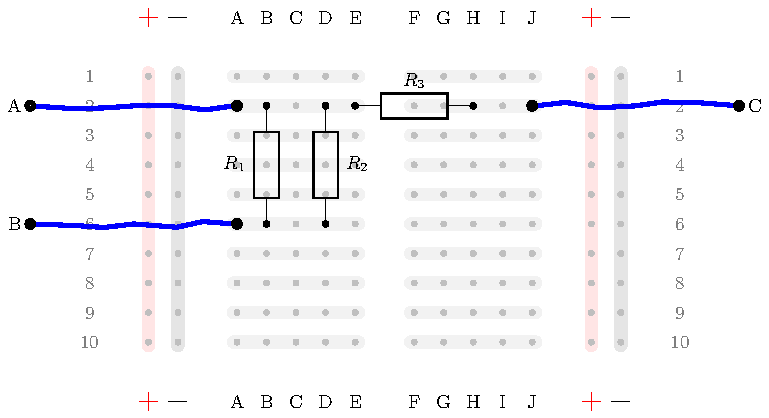
\includegraphics[width=0.95\textwidth]{kuvat/kuva3.pdf}
\end{center}


\begin{tcolorbox}[colback=yellow!10, title={Testaa taitosi!},colbacktitle=orange]
Piirrä kuvan mukainen kytkentä koekytkentälevylle.
\centering
\begin{tikzpicture}
\draw (0,0) node[anchor=east] {B} to [short, o-] (1,0) to[R=$R_1$] (1,2);

\draw (0,2) node[anchor=east] {A} to [short,o-*] (1,2);
\draw (1,2) to[R=$R_2$,*-] (4,2) to[short,-o] (6,2) node[right] {C};
\draw (4,2) to[R,a=$R_3$,*-] (4,0) --(5,0) to[R,a=$R_4$,*-*] (5,2);
\draw (5,0) to[short,-o] (6,0) node[right] {D};
\end{tikzpicture}

\begin{tikzpicture}[scale=0.5]
\BREADBOARD (0,0) {15};

\unless\ifHideSolutions
\draw (B10) to[R=$R_1$,*-*] (B14);
\draw[blue,wire] (A10) to[short,*-o] ++(-7,0) node[left,black] {A};
\draw[blue,wire] (A14) to[short,*-o] ++(-7,0) node[left,black] {B};
\draw (C10) to[R=$R_2$,*-*] (C6);
\draw (B6) to [R=$R_3$,*-*] (B2);
\draw (D6) to [R=$R_4$,*-*] (D2);
\draw[blue,wire] (A6) to[short,*-o] ++(-7,0) node[left,black] {C};
\draw[blue,wire] (A2) to[short,*-o] ++(-7,0) node[left,black] {D};
\fi

\end{tikzpicture}\\
\begin{solution}
Kuvassa on esitetty yksi esimerkki, mutta myös muita vaihtoehtoja on olemassa.
\end{solution}
\end{tcolorbox}

\begin{tcolorbox}[colback=yellow!10, title={Testaa taitosi!},colbacktitle=orange,]
Merkitse koekytkentälevylle johdot solmuihin A, B, C ja D.

\centering
\begin{tikzpicture}
\draw (0,0) node[anchor=east] {A} to [short, o-] (1,0) to[R=$R_1$] (1,2);
\draw (0,3) node[anchor=east] {B} to [short,o-*] (1,3);
\draw (1,2) to[R=$R_2$,*-] (4,2) to[short,-o] (6,2) node[right] {C};
\draw (1,2) to[short,*-] (1,3) to[R=$R_3$] (4,3) to[short,-*] (4,2);
\draw (4,2) to[R,a=$R_4$,*-] (4,0) --(5,0) to[R,a=$R_5$,*-*] (5,2);
\draw (5,0) to[short,-o] (6,0) node[right] {D};
\end{tikzpicture}

\begin{tikzpicture}[scale=0.5]
\BREADBOARD (0,0) {15};

\draw (B10) to[R=$R_1$,*-*] (B14);
\draw (C10) to[R=$R_2$,*-*] (C6);
\draw (E10) to[R,a=$R_3$,*-*] (E6);
\draw (B6) to [R=$R_4$,*-*] (B2);
\draw (D6) to [R,a=$R_5$,*-*] (D2);
\unless\ifHideSolutions

\draw[blue,wire] (A10) to[short,*-o] ++(-7,0) node[left,black] {B};
\draw[blue,wire] (A14) to[short,*-o] ++(-7,0) node[left,black] {A};

\draw[blue,wire] (A6) to[short,*-o] ++(-7,0) node[left,black] {C};
\draw[blue,wire] (A2) to[short,*-o] ++(-7,0) node[left,black] {D};
\fi

\end{tikzpicture}\\
\begin{solution}
Kuvassa on esitetty yksi esimerkki, mutta myös muita vaihtoehtoja on olemassa.
\end{solution}
\end{tcolorbox}


\begin{tcolorbox}[colback=yellow!10, title={Testaa taitosi!},colbacktitle=orange]
Jos edelliseen piiriin pitäisi lisätä vastus olemassa olevan solmun D ja uuden solmun E välille, mihin väliin kytkisit uuden vastuksen?

\begin{tikzpicture}[scale=0.5]
\BREADBOARD (0,0) {15};

\draw (B10) to[R=$R_1$,*-*] (B14);
\draw (C10) to[R=$R_2$,*-*] (C6);
\draw (E10) to[R,a=$R_3$,*-*] (E6);
\draw (B6) to [R=$R_4$,*-*] (B2);
\draw (D6) to [R,a=$R_5$,*-*] (D2);
\unless\ifHideSolutions
\draw (E2) to [R=R,*-*] (H2);
\draw[blue,wire] (A10) to[short,*-o] ++(-7,0) node[left,black] {B};
\draw[blue,wire] (A14) to[short,*-o] ++(-7,0) node[left,black] {A};

\draw[blue,wire] (A6) to[short,*-o] ++(-7,0) node[left,black] {C};
\draw[blue,wire] (A2) to[short,*-o] ++(-7,0) node[left,black] {D};
\draw[blue,wire] (J2) to[short,*-o] ++(7,0) node[right,black] {E};
\fi

\end{tikzpicture}\\
\begin{solution}
Kuvassa on esitetty yksi esimerkki, mutta myös muita vaihtoehtoja on olemassa.

\centering
\begin{tikzpicture}
\draw (0,0) node[anchor=east] {A} to [short, o-] (1,0) to[R=$R_1$] (1,2);
\draw (0,3) node[anchor=east] {B} to [short,o-*] (1,3);
\draw (1,2) to[R=$R_2$,*-] (4,2) to[short,-o] (6,2) node[right] {C};
\draw (1,2) to[short,*-] (1,3) to[R=$R_3$] (4,3) to[short,-*] (4,2);
\draw (4,2) to[R,a=$R_4$,*-] (4,0) --(5,0) to[R,a=$R_5$,*-*] (5,2);
\draw (5,0) to[short,-o] (6,0) node[right] {D};
\draw (5,0) to[short] (5,-0.5) to[R,a=R] (7,-0.5) to[short,-o] (8,-0.5) node[below] {E}; 
\end{tikzpicture}

\end{solution}
\end{tcolorbox}

\clearpage
\section{Koekytkentälevystä}

\begin{itemize}
    \item Yksi rivi (A-B-C-D-E) tai (F-G-H-I-J) vastaa yhtä solmua piirroksessa.
    \item Jos yhteen solmuun kiinnittyy enintään viisi (5) viivaa, riittää käyttää kaikki valmiina olevat paikat (A-E tai F-J). 
    \item Jos yhdessä solmussa on yli viisi (5) viivaa, tee lisä tilaa lisäämällä johto (eli oikosulku) esimerkiksi saman rivin toiselle puolelle (esimerkiksi käytössä rivi 3: kytke johto E3:sta F3:een, ja sinulla on nyt vapaana A3, B3, C3, D3, G3, H3, I3 ja J3.
    \item $+$ tai $-$ pystyrivejä käytetään yleensä käyttöjännitteelle (punainen $+$) sekä maalle (musta $-$). Näistä lisää seuraavaksi.
\end{itemize}

\begin{center}
\begin{tikzpicture}[scale=0.5]
\BREADBOARD (0,0) {15};
\end{tikzpicture}
\end{center}

\section{Ensimmäinen kytkentä koekytkentälevylle}

\begin{minipage}{0.5\textwidth}
\begin{tcolorbox}[colback=lime!10,title=Tarvikkeet, colbacktitle=green!10,coltitle=black]
\begin{itemize}
    \item Yleismittari (vastuksen arvon selvittämiseen)
    \item Vastus $220\Omega$: 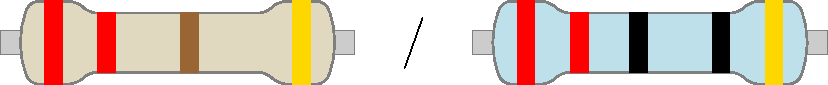
\includegraphics[width=0.5\textwidth]{kuvat/220.pdf}
    \item Koekytkentälevy
    \item Arduino UNO (jännitelähteenä)
    \item LED
    \item Hyppylankoja
\end{itemize}
\end{tcolorbox}
\end{minipage}
\begin{minipage}{0.5\textwidth}
\begin{tcolorbox}[colback=blue!10,title=Piirin toiminta,colbacktitle=purple!90]
LEDin harjoituskytkentä. LED palaa, kun piiri on kytketty jännitelähteeseen.
\tcblower
\begin{center}
\begin{tikzpicture}
\ctikzset{american}
\draw (0,0) to[R,l=$220\Omega$] (0,-2) to [led] (0,-4);
\draw (-2,0) to[V,l=$5V$] (-2,-4); 
\draw (-2,0) to[short] (0,0);
\draw (-2,-4) to[short] (0,-4);
\end{tikzpicture}
\end{center}
\end{tcolorbox}
\end{minipage}

\begin{tcolorbox}[colback=red!10,colbacktitle=red,title=HUOM!]
Aina kun rakennat tai muutat piiriä, pidä Arduino irrotettuna tietokoneesta! 
\tcblower
LEDin kanssa kytketään aina sarjaan vastus (nyt $220\Omega$), kun kytket LEDin $5V$- jännitteeseen.
\end{tcolorbox}

\begin{tcolorbox}[title=Vastuksen arvo]
Jos sinulla ei ole käytössä yleismittaria oikean vastuksen arvon mittaamiseen, tai haluat harjoitella vastusten värikoodien lukemista, vastusten värikoodit löydät sivulta \pageref{varikoodit}.

Nyt tarvitaan $220\Omega$ vastus eli jompikumpi alla olevista vaihtoehdoista:

\begin{center}
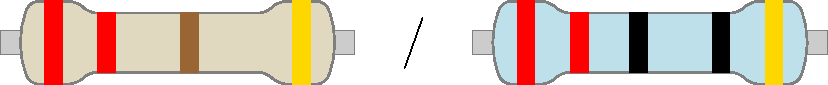
\includegraphics[width=0.5\textwidth]{kuvat/220.pdf}
\end{center}
\end{tcolorbox}

\begin{tcolorbox}[title=LEDin kytkeminen,colback=blue!10,colbacktitle=purple!90]\label{box:led}
Huomaa, että on merkitystä kummin päin LED kytketään koekytkentälevylle! 

LEDissä on kaksi jalkaa, joista toinen on pidempi. LEDin muovi on toiselta puolelta kaareva, ja toiselta siinä on suora leikkaus, lyhyempi jalka on suoran leikkauksen puolella. Lyhyemmän jalan nimi on katodi ja pidemmän jalan anodi.

\begin{minipage}{0.5\textwidth}
Piirrosmerkissä:
\begin{center}
\begin{tikzpicture}
%\node at (-1,0) {anodi};
\draw (0,0) node[left,text width=1.5cm] {anodi\\ pitkä jalka} to[led,o-o] (2,0) node[right,text width=2cm] {katodi\\lyhyt jalka};
\end{tikzpicture}
\end{center}
\end{minipage}
\begin{minipage}{0.5\textwidth}
\begin{tikzpicture}
\node (led) at (0,0) {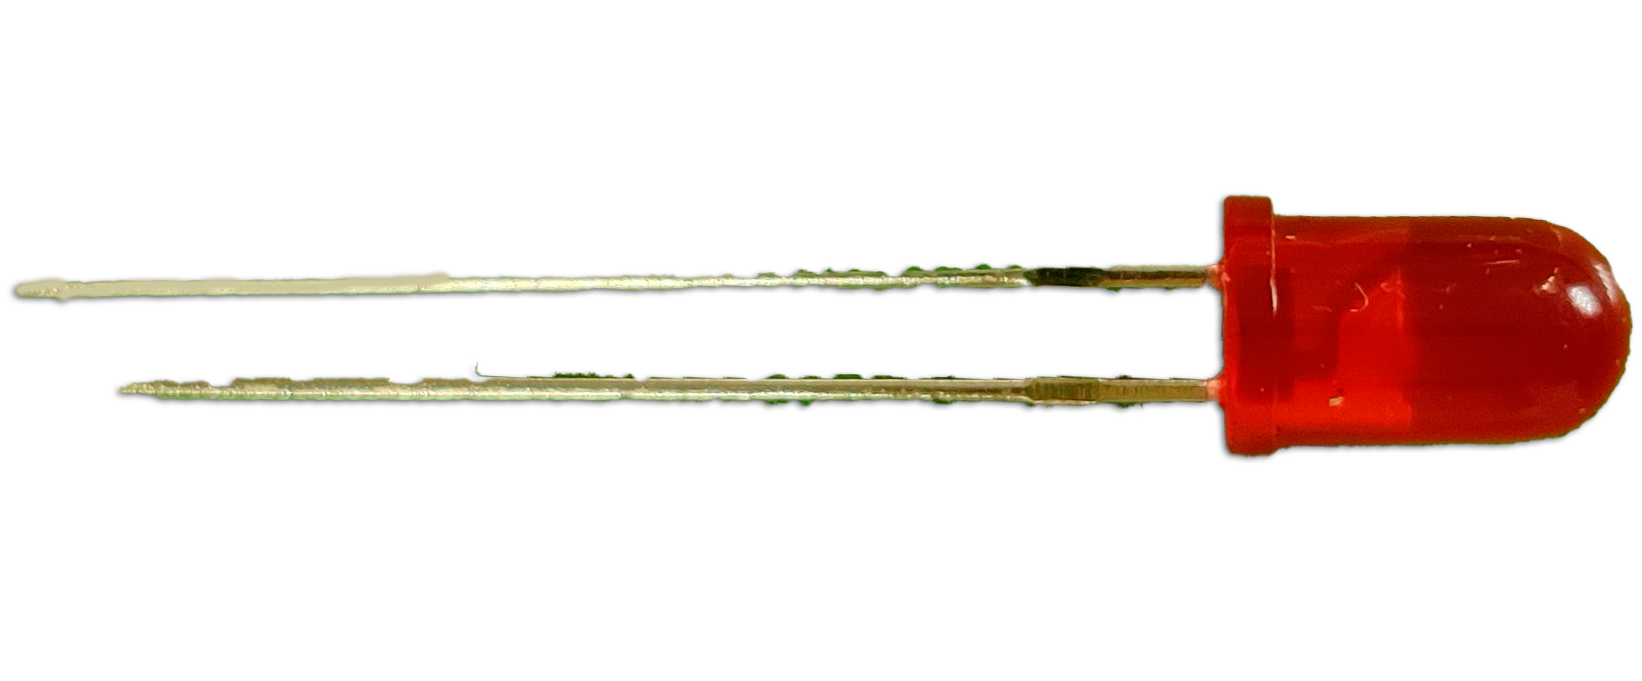
\includegraphics[width=0.95\textwidth]{kuvat/led.png}};
\node[above=0.5] (led) {Anodi (pitkä jalka)};
\node[below=0.5] (led) {Katodi (lyhyt jalka) + tasainen puoli};
\end{tikzpicture}
\end{minipage}

LED, eli valoa säteilevä diodi päästää virtaa läpi vain toiseen suuntaan kuten diodit. Jos anodille kytketään tarpeeksi suuri jännite verrattuna katodiin, virta kulkee ja valo palaa. Jos taas katodilla on suurempi jännite kuin anodilla, virtaa ei kulje ja LED ei pala. Jos anodilla ei ole tarpeeksi suuri jännite verrattuna katodiin, virta ei kulje. Riippuen LEDistä, vaadittu kynnysjännite voi vaihdella ja on tyypillisesti 1,5-4,5 volttia. 
\end{tcolorbox}

\begin{tcolorbox}[title=Jännitelähteen kytkeminen]
Jännitelähde on Arduinossa sisäänrakennettuna. Jotta voimme kytkeä jännitelähteen piiriin, tarvitsemme jännitelähteen molemmat päät: +5V ja maan (GND), kytkemällä vain toinen piiriin emme saa aikaan haluttua vaikutusta.

Arduino levyllä on kolme eri GND-riviä, ja mikä tahansa niistä käy. Kuvassa selvyyden vuoksi ne on numeroitu.

\begin{minipage}{0.3\textwidth}
\begin{tikzpicture}
\ctikzset{american}
\draw (-2,0.5) node[above] {5V} to[short,o-]  (-2,0) to[V,l=$5V$] (-2,-2) to[short,-o] (-2,-2.5) node[below] {GND};
%\node (-2,0.5) {5V};
\end{tikzpicture}
 \end{minipage}
\begin{minipage}{0.7\textwidth}
\begin{tikzpicture}[scale=0.5]
\pic[scale=0.2] at (0,0) {myarduino};
\draw[red,wire] (Ar5V) to[short,*-o] ++(-5,0) node[left,black] {5V};
\draw[black,wire] (ArGND2) to[short,*-o] ++(-5,0) node[left,black] {GND};
\end{tikzpicture}
\end{minipage}
\end{tcolorbox}

%\begin{tcolorbox}[colback=yellow!10, title={Tee kytkentä!},colbacktitle=orange]
Kytketään ensin vastus ja LED kuvan mukaisesti ja lisätään kaksi hyppylankaa.

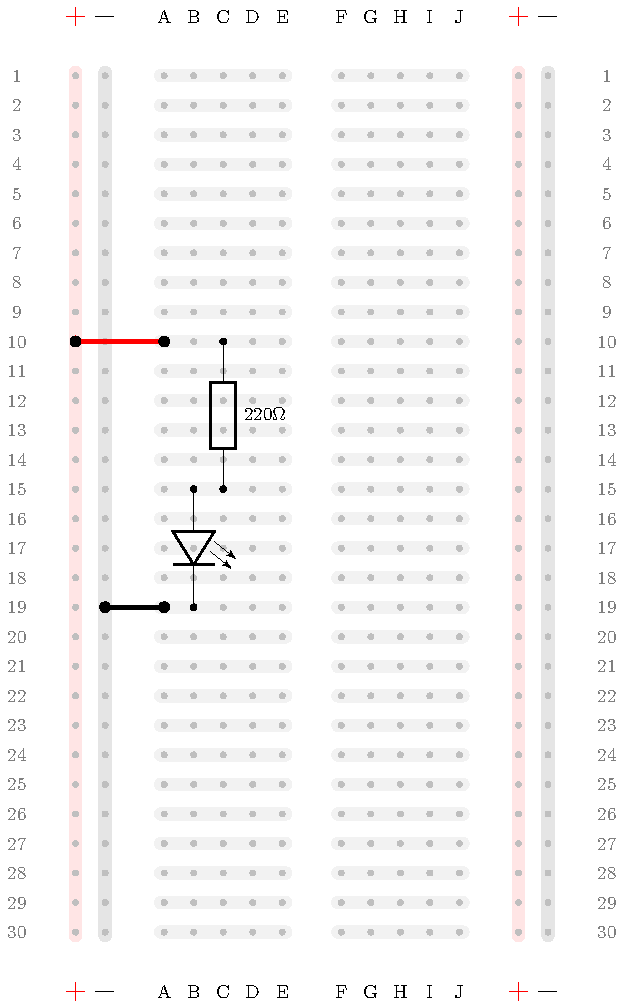
\includegraphics[width=0.8\textwidth]{kuvat/kuva4.pdf}


Nyt on siis tehty muuten kytkennät ja pitää kiinnittää vielä jännitelähde piiriin.
%\end{tcolorbox}

Kytketään nyt käyttöjännite (+5V) vasemmalle $+$ pystyriville ja maa (GND) tämän viereiselle $-$ pystyriville.

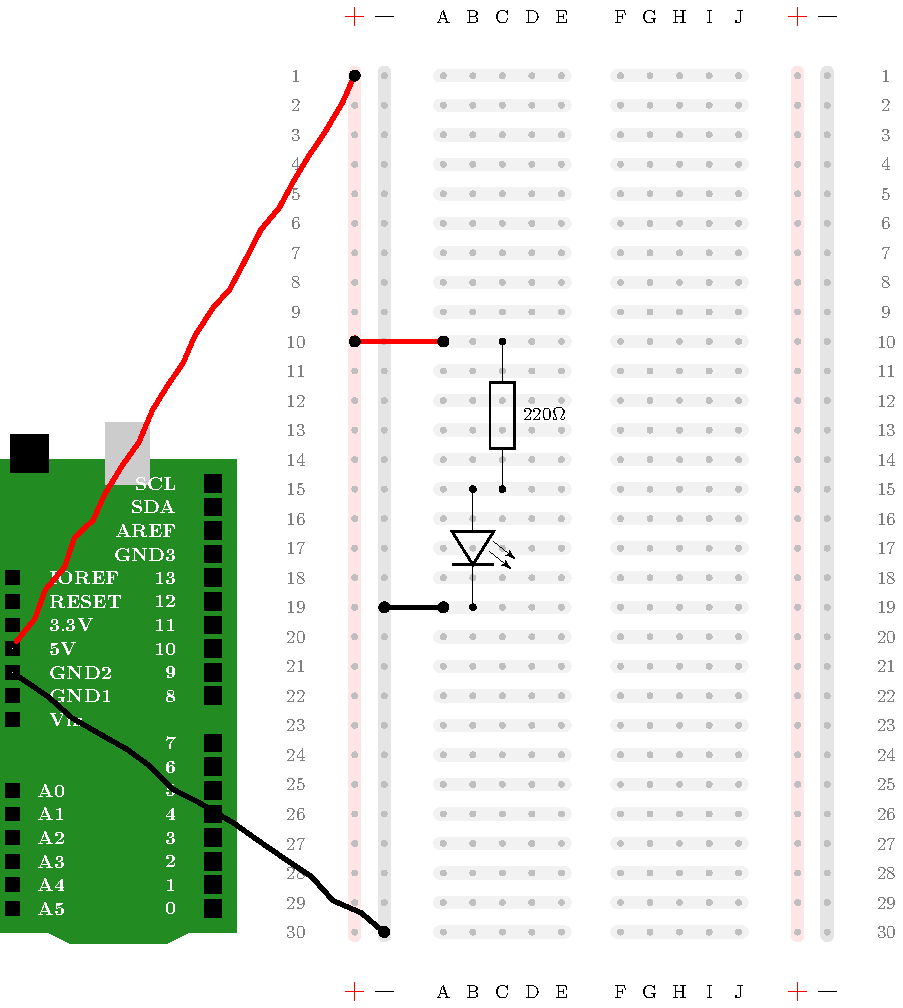
\includegraphics[width=0.95\textwidth]{kuvat/kuva5.pdf}

Nyt kun yhdistetään Arduino johdolla tietokoneeseen, LED syttyy!

\section{Lisätään kytkentään painonappi}

\begin{minipage}{0.5\textwidth}
\begin{tcolorbox}[colback=lime!10,title=Tarvikkeet, colbacktitle=green!10,coltitle=black]
\begin{itemize}
    \item Edellisen työn koottu piiri
    \item Painonappi
\end{itemize}
\end{tcolorbox}
\end{minipage}
\begin{minipage}{0.5\textwidth}
\begin{tcolorbox}[colback=blue!10,title=Piirin toiminta,colbacktitle=purple!90]
Painonapin koekytkentä. Nappia painamalla LED syttyy.
\tcblower
\begin{center}
\begin{tikzpicture}
\ctikzset{american}
\draw (0,0) to[R,l=$220\Omega$] (0,-2) to [led] (0,-4);
\draw (-2,0) to[V,l=$5V$] (-2,-4); 
\draw (-2,0) to[nopb] (0,0);
\draw (-2,-4) to[short] (0,-4);
%\draw (-2,0) to[nopb] (-2,3);
\end{tikzpicture}
\end{center}
\end{tcolorbox}
\end{minipage}

\begin{tcolorbox}[colback=red!10,colbacktitle=red,title=HUOM!]
Aina kun rakennat tai muutat piiriä, pidä Arduino irrotettuna tietokoneesta! 
\end{tcolorbox}

Nyt lisätään piiriin painonappi. 

\begin{tcolorbox}[title=Painonapin kytkeminen,colback=blue!10,colbacktitle=purple!90]
Arduinon mukana tulevassa painonapissa on neljä pinniä, ja asetetaan keskellä olevan uran ylitse. Jos nappia ei paineta, niin A-E ja F-J rivillä 2 ovat samaa pistettä, mutta eri pistettä kuin rivin 4 (A-E) ja (F-J). Jos nappia painetaan, niin molempien rivien (2 ja 4) kaikki pisteet ovat kiinni toisissaan.


\begin{tikzpicture}[scale=0.5]
\BREADBOARD (0,0) {5};
\draw[thick,fill=hopea] (E2.east) rectangle (F4.west) coordinate[pos=0.5] (Y);
\draw[fill=black] (Y) circle (0.5);
\draw (E2.east) to[short,*-*] (E2);
\draw (E4.east) to[short,*-*] (E4);
\draw (F4.west) to[short,*-*] (F4);
\draw (F2.west) to[short,*-*] (F2);
\end{tikzpicture}
\end{tcolorbox}

Siirretään lyhyempää punaista johtoa kohdasta A10 kohtaan A8. Lisätään painonappi pisteisiin E8, E10, F8 ja F10.

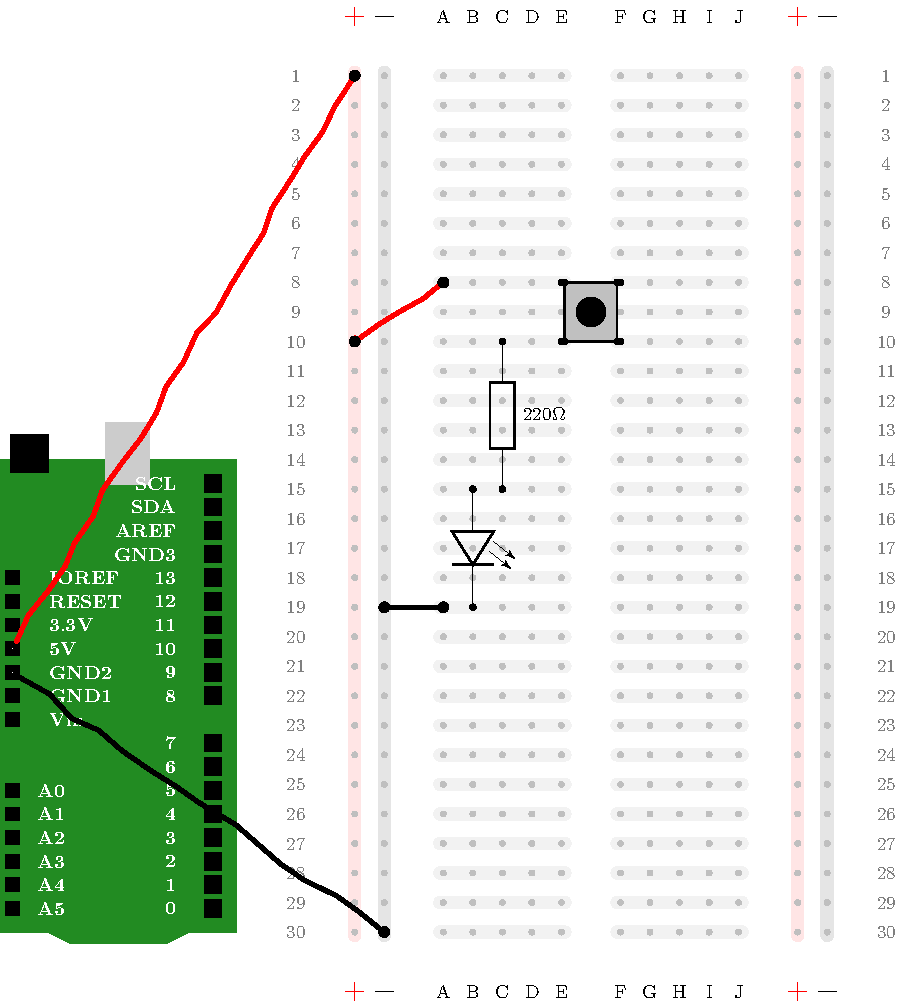
\includegraphics[width=0.95\textwidth]{kuvat/kuva6.pdf}

Nyt kytke Arduino takaisin kiinni koneeseen, ja saat LEDin syttymään painamalla nappulaa. 


\chapter{Liikennevalot}

Lähdetään rakentamaan risteykseen ohjattuja liikennevaloja. Tässä osiossa aloita tyhjästä koekytkentälevystä.

\section{Ohjelmoitava valo}
\begin{minipage}{0.5\textwidth}
\begin{tcolorbox}[colback=lime!10,title=Tarvikkeet, colbacktitle=green!10,coltitle=black]
\begin{itemize}
    \item Punainen LED
    \item Vastus 220$\Omega$: 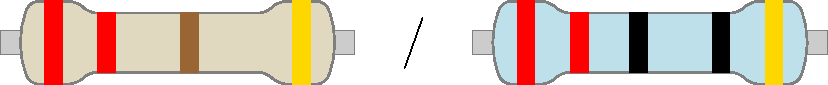
\includegraphics[width=0.5\textwidth]{kuvat/220.pdf}
    \item Hyppylankoja
    \item Arduino + koekytkentälevy
\end{itemize}
\end{tcolorbox}
\end{minipage}
\begin{minipage}{0.5\textwidth}
\begin{tcolorbox}[colback=blue!10,title=Piirin toiminta,colbacktitle=purple!90]
Ensimmäinen ohjelmoitava piiri. Kirjoitetaan koodi, joka sytyttää ja sammuttaa valon koodin mukaisesti.
\tcblower
\begin{center}
\begin{tikzpicture}
\ctikzset{american}
\draw (0,4) to [led,l=punainen,fill=red] (0,2);
\draw (0,2) to[R,a=$220\Omega$] (0,0);
\draw (0,0) -- (0,-0.5) node[ground]{}; 
\draw (-1,4) node[left] {7} to[short,o-] (0,4);
\end{tikzpicture}
\end{center}
\end{tcolorbox}
\end{minipage}

\begin{tcolorbox}[colback=red!10,colbacktitle=red,title=HUOM!]
Aina kun rakennat tai muutat piiriä, pidä Arduino irrotettuna tietokoneesta! 
\tcblower
Muista tarkistaa miten päin LEDit kytketään! Tämä löytyy esimerkiksi sivulta \pageref{box:led}.
\end{tcolorbox}

Aiemmin käytimme painonappia valon ohjaamiseen, ja painamalla nappia saimme valon syttymään. Nyt tehdään kytkentä, jonka avulla saadaan valo automaattisesti sammumaan ja syttymään. 


Kytketään ensin punainen LED ja vastus koekytkentälevylle. Ja kytketään myös $-$ maahan.

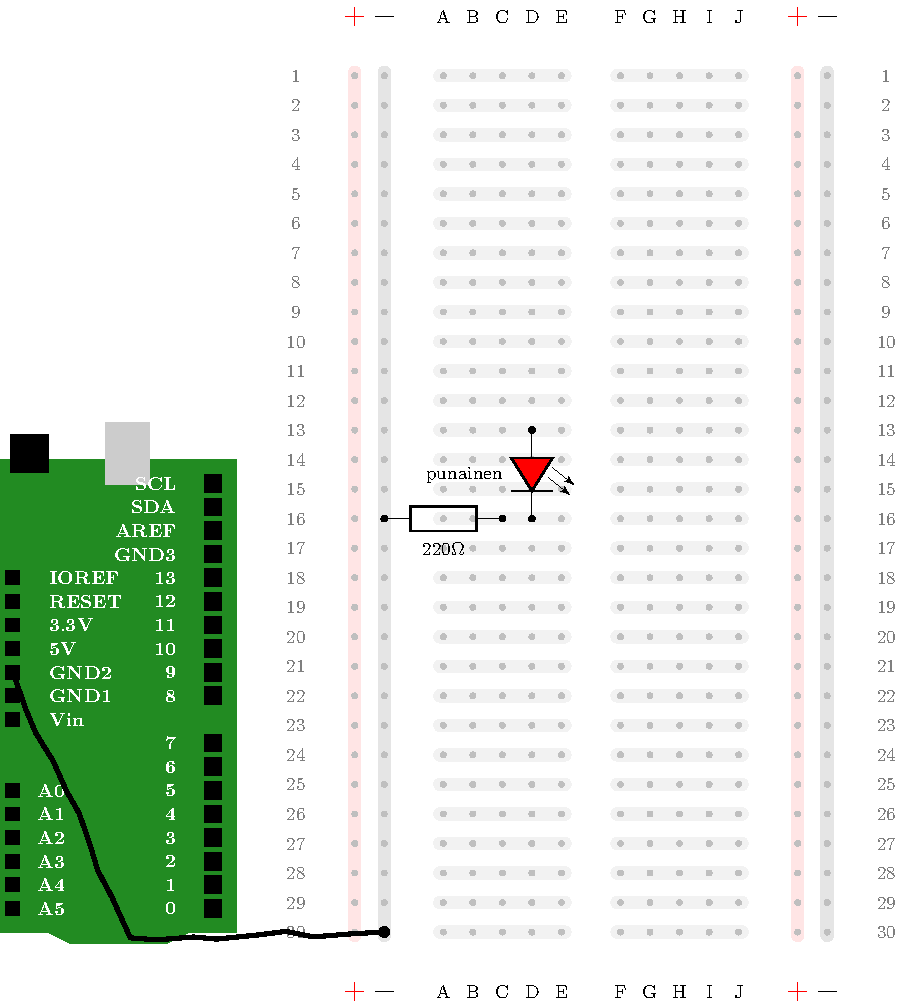
\includegraphics[width=0.95\textwidth]{kuvat/kuva7.pdf}

Aiemmassa kytkennässä rivi 13 kytkettiin suoraan vakiojännitelähteeseen, 5V, mutta nyt koska haluamme ohjelmoida, kytketään rivi 13 käyttämältämme puolelta ohjelmoitavaan pinniin 7 Arduinossa.

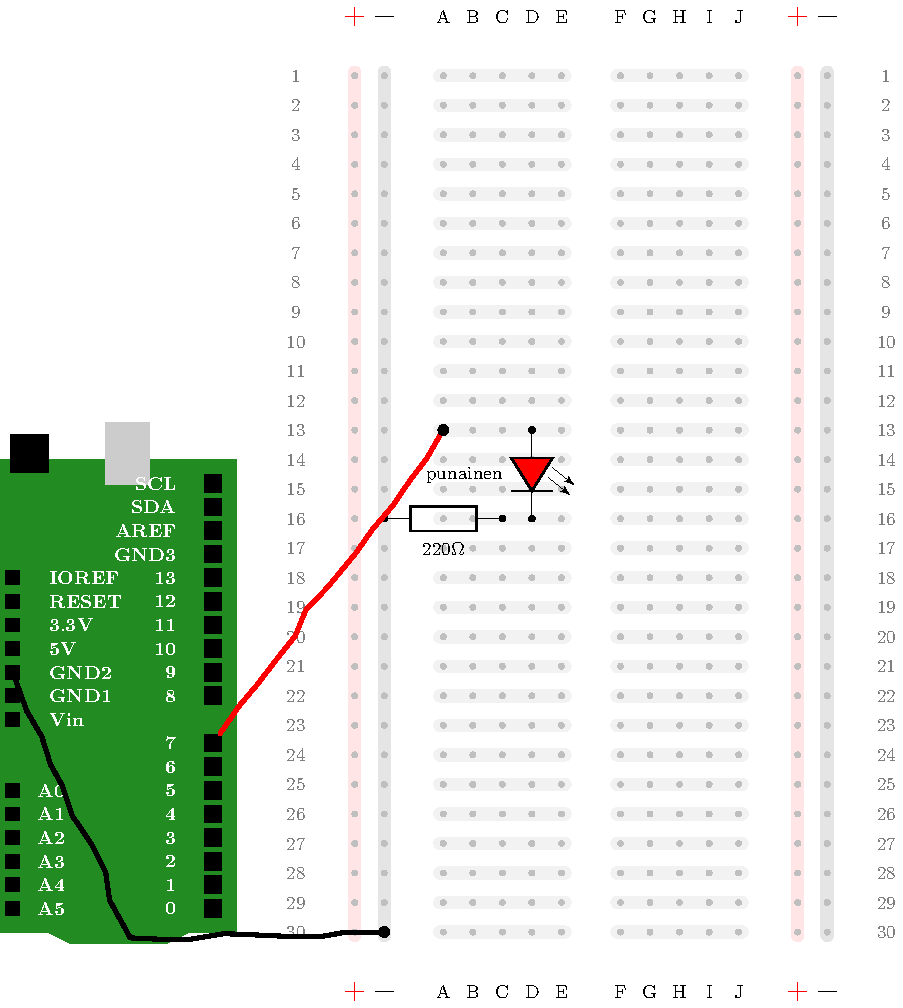
\includegraphics[width=0.8\textwidth]{kuvat/kuva8.pdf}

Avataan nyt Arduino-sovellus, ja kopioidaan alla oleva koodi sinne.


\begin{lstlisting}[numbers=none]
void setup() {
pinMode(7, OUTPUT); // Punainen LED on pinnissa 7
}

void loop() {
digitalWrite(7, HIGH); // Laitetaan valo paalle
delay(1000); // Odotetaan
digitalWrite(7, LOW); // Laitetaan valo pois paalta
delay(1000); // Odotetaan
}
\end{lstlisting}


Käydään vielä koodi lävitse: 

Rivit 1-3 ovat alustamista (asetukset) varten. Rivillä 3 kerrotaan mitä haluamme tehdä pinnillä 7: haluamme ohjata tällä valoa, joten tyyppi on OUTPUT.

Rivit 5-10 ovat miten haluamme ohjata valoa. Kirjoittamalla rivin 6 koodin, asetamme pinnin 7 arvoksi HIGH, eli korkea, eli 5V, ja kuten tiedämme aiemmasta piiristämme, tällöin valo palaa. Sitten seuraavalla rivillä odotamme 1000ms (millisekuntia, eli yhden sekunnin), kunnes teemme rivin 8 operaation: muutamme pinnin 7 arvoksi LOW, eli matala, eli 0V, ja sammutamme valon. Tämän jälkeen odotamme taas yhden sekunnin. Koska koodi on kirjoitettu silmukkaan (loop), toistamme tätä, kunnes kytkemme piirin irti jännitelähteestä.

Nyt voit ladata Arduinolle koodin ja katsoa mitä tapahtuu! Voit myös testata odotusajan muuttamista muuttamalla lukuja 1000 koodissa. Muista, että kyseessä on millisekunnit, joten jos haluat, että valo on päällä 3s ja pois päältä 2s, ensimmäinen 1000 pitää muuttaa luvuksi 3000 ja toinen luvuksi 2000. 

\begin{tcolorbox}[colback=white,title=Vinkkejä Arduinolla koodaamiseen!,colbacktitle=purple!90]
Seuraavassa esitellään Arduinolla koodaamiseen liittyviä vinkkejä. 
\begin{lstlisting}
// Kaksi kauttaviivaa aloittaa kommentin. Tata ei siis lueta koodissa vaan on tiedoksi koodin lukijalle

pinMode(luku, tyyppi) // Talla voit saataa pinnien 0-13 tekoa laittamalla sanan luku tilalle luvun jolta rivilta haluat komentaa
// Tyypin tilalle voit kirjoittaa joko OUTPUT eli Arduino lahettaa signaalia
// tai INPUT jolloin Arduino vastaanottaa signaalin

digitalWrite(luku, arvo) // Talla voit muuttaa pinniin luku kirjoitettua arvoa
// arvo HIGH vastaa 5V jannitetta
// arvo LOW vastaa 0V jannitetta

delay(luku) // Odottaa luvun verran millisekunteja
\end{lstlisting}
\end{tcolorbox}

\section{Ohjelmoitava liikennevalo}

\begin{tcolorbox}[colback=lime!10,title=Tarvikkeet, colbacktitle=green!10,coltitle=black]
\begin{itemize}
    \item Edellisen kohdan piiri rakennettuna
    \item Keltainen LED ja vihreä LED
    \item 2 kpl 220$\Omega$: 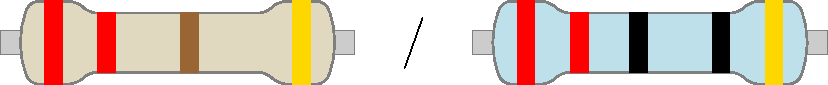
\includegraphics[width=0.5\textwidth]{kuvat/220.pdf}
    \item Hyppylankoja
\end{itemize}
\end{tcolorbox}


\begin{tcolorbox}[colback=blue!10,title=Piirin toiminta,colbacktitle=purple!90]
Kirjoitetaan koodi, jonka avulla saadaan liikennevalot toimimaan.
\tcblower
\begin{center}
\begin{tikzpicture}[]
\ctikzset{american}
\draw (0,4) to [led,l=punainen,fill=red] (0,2);
\draw (0,2) to[R,a=$220\Omega$] (0,0);
\draw (0,0) -- (0,-0.5) node[ground]{}; 
\draw (-1,4) node[left] {7} to[short,o-] (0,4);

\draw (3,4) to [led,l=keltainen,fill=yellow] (3,2);
\draw (3,2) to[R,a=$220\Omega$] (3,0);
\draw (3,0) -- (3,-0.5) node[ground]{}; 
\draw (2,4) node[left] {4} to[short,o-] (3,4);

\draw (6,4) to [led,l=vihreä,fill=green] (6,2);
\draw (6,2) to[R,a=$220\Omega$] (6,0);
\draw (6,0) -- (6,-0.5) node[ground]{}; 
\draw (5,4) node[left] {3} to[short,o-] (6,4);

\end{tikzpicture}
\end{center}
\end{tcolorbox}


\begin{tcolorbox}[colback=red!10,colbacktitle=red,title=HUOM!]
Aina kun rakennat tai muutat piiriä, pidä Arduino irrotettuna tietokoneesta! 
\end{tcolorbox}

Lisätään ensin keltainen ja vihreä LED ja niiden kanssa sarjassa olevat vastukset ja kytketään keltainen LED pinniin 4 ja vihreä LED pinniin 3. Huomaa, että hyppylankojen värillä ei ole väliä. Selvyyden vuoksi kuvassa on käytetty samaa väriä kuin mihin LEDiin ollaan yhdistämässä.

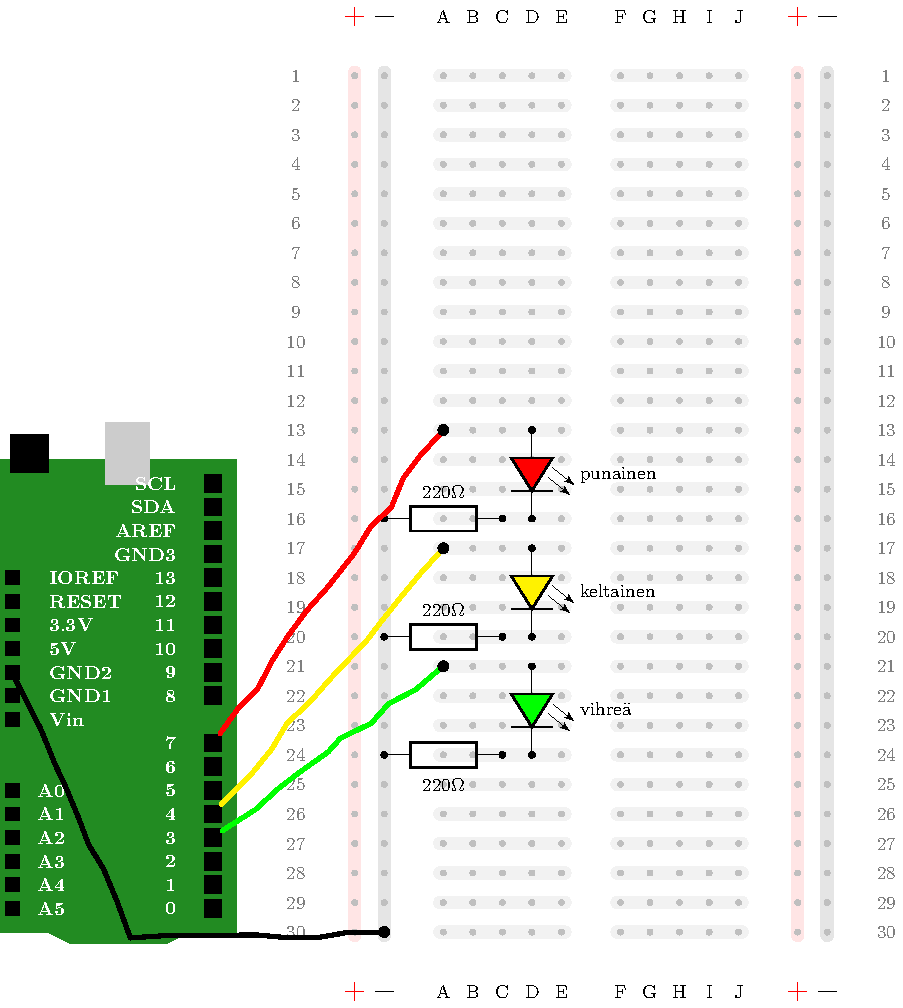
\includegraphics[width=0.95\textwidth]{kuvat/kuva9.pdf}

Nyt lisätään keltaiselle ja vihreällä LEDille (vastaavasti kuin punaisella LEDillä jo on), tieto siitä mitä pinneillä 4 ja 3 halutaan tehdä.
\clearpage
\begin{lstlisting}[numbers=none] 
void setup() {
pinMode(7, OUTPUT); // Punainen LED on pinnissa 7
pinMode(4, OUTPUT); // Keltainen LED on pinnissa 4
pinMode(3, OUTPUT); // Vihrea LED on pinnissa 2
}

void loop() {
digitalWrite(7, HIGH); // Laitetaan punainen valo paalle
digitalWrite(4, HIGH); // Laitetaan keltainen valo paalle
digitalWrite(3, HIGH); // Laitetaan vihrea valo paalle
delay(1000); // Odotetaan
digitalWrite(7, LOW); // Laitetaan punainen valo pois paalta
digitalWrite(4, LOW); // Laitetaan keltainen valo pois paalta
digitalWrite(3, LOW); // Laitetaan vihrea valo pois paalta
delay(1000); // Odotetaan
}
\end{lstlisting}

Nyt yllä oleva koodi vilkuttaa kaikkea kolmea valoa yhtä aikaa. Vaihda rivien järjestystä, ja lisää tarvittaessa odotuskomentoja tai päälle/pois komentoja, jotta saat valot ohjelmoitua. 

\begin{tcolorbox}[colback=yellow!10, title={Koodaa!},colbacktitle=orange]
Miten muutat koodia, jotta saat liikennevalot toimimaan kuten oikeat valot toimivat? 
\begin{solution}
\begin{lstlisting}
void setup() {
pinMode(7, OUTPUT); // Punainen LED on pinnissa 7
pinMode(4, OUTPUT); // Keltainen LED on pinnissa 4
pinMode(3, OUTPUT); // Vihrea LED on pinnissa 2
}

void loop() {
digitalWrite(7, HIGH); // Laitetaan punainen valo paalle
delay(1000); // Odotetaan
digitalWrite(4, HIGH); // Laitetaan keltainen valo paalle
delay(1000); // Odotetaan
digitalWrite(7, LOW); // Laitetaan punainen valo pois paalta
digitalWrite(4, LOW); // Laitetaan keltainen valo pois paalta
digitalWrite(3, HIGH); // Laitetaan vihrea valo paalle
delay(1000); // Odotetaan
digitalWrite(3, LOW); // Laitetaan vihrea valo pois paalta
digitalWrite(4, HIGH); // Laitetaan keltainen valo paalle
delay(1000);
digitalWrite(4, LOW); // Laitetaan keltainen valo pois paalta
digitalWrite(7, HIGH); // Laitetaan punainen valo paalle
delay(1000); // Odotetaan
}

\end{lstlisting}
Kyseessä on esimerkkikoodi, ja tämän jälkeen voidaan puhua siitä, kauanko kukin valo palaa ja tarvitseeko viimeisenä olla punainen valo päälle vai ei.
\end{solution}
\end{tcolorbox}

%%%%%%%%%%%%%%%%%%%%%%%%%%%%%%%%%5
\clearpage
\section{Painonapin lisääminen}
\begin{tcolorbox}[colback=lime!10,title=Tarvikkeet, colbacktitle=green!10,coltitle=black]
\begin{itemize}
    \item Edellisen kohdan piiri rakennettuna
    \item Painonappi
    \item Vastus 220$\Omega$: 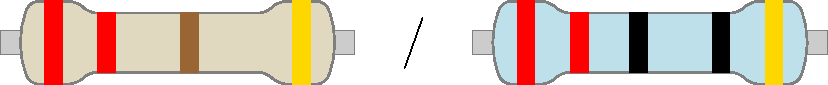
\includegraphics[width=0.5\textwidth]{kuvat/220.pdf}
    \item Hyppylankoja
\end{itemize}
\end{tcolorbox}


\begin{tcolorbox}[colback=blue!10,title=Piirin toiminta,colbacktitle=purple!90]
Lisätään painonappi, jota painamalla saadaan liikennevalojen toiminta muuttumaan.
\end{tcolorbox}

\begin{tcolorbox}[colback=red!10,colbacktitle=red,title=HUOM!]
Aina kun rakennat tai muutat piiriä, pidä Arduino irrotettuna tietokoneesta! 
\end{tcolorbox}

Käytimme jo aiemmin painonappia manuaalisesti valon ohjaamiseen, mutta lisätään tämä nyt koodimme. Lisää aiempaan kytkentääsi painonappi sekä vastus ja kolme hyppylankaa (kuvassa punainen ja kaksi sinistä).

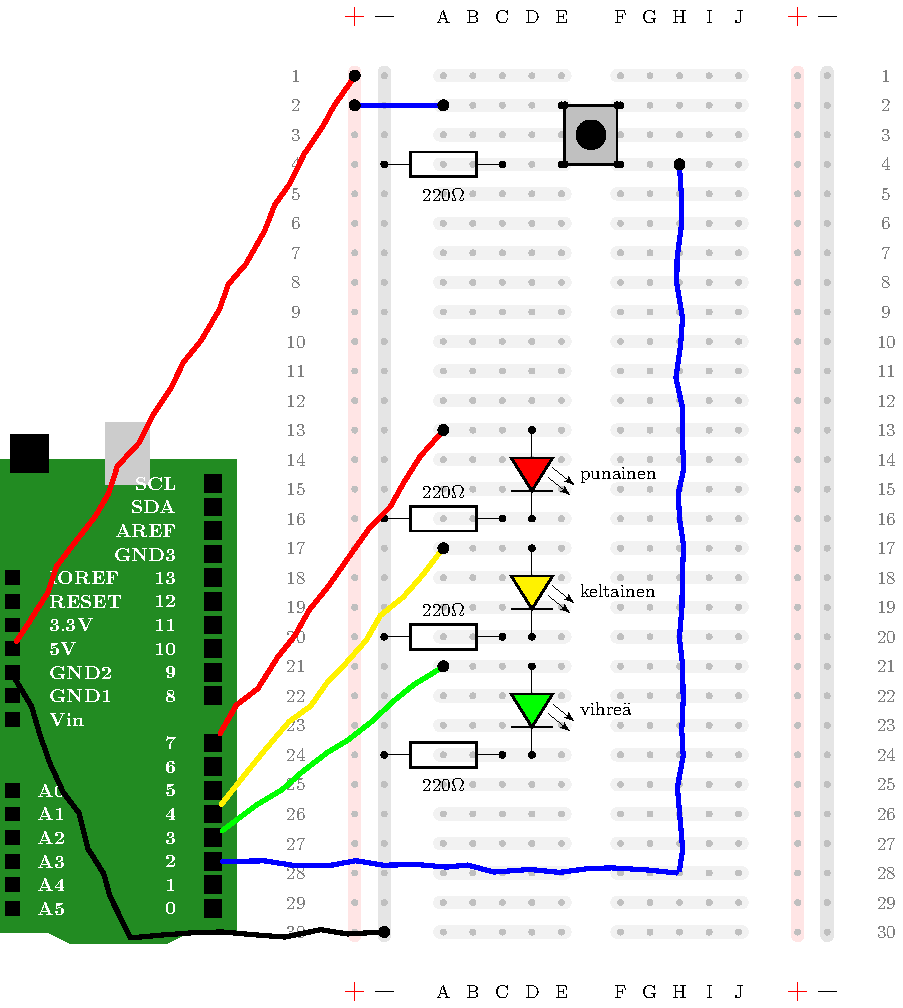
\includegraphics[width=0.9\textwidth]{kuvat/kuva10.pdf}

% \begin{tikzpicture}[scale=0.5]
% \pic[scale=0.2] at (0,0) {myarduino};
% \BREADBOARD(20,30){30};
% \draw (C16) to[R,a=$220\Omega$,*-*] (lg16);
% \draw (D13) to[led,l=punainen,*-*,fill=red] (D16);
% \draw[black,wire] (ArGND2) -- ++(4,-9) to[short,-*] (lg30);
% \draw[wire,red] (A13) to[short,*-*] (Ar7);

% \draw (C20) to[R,a=$220\Omega$,*-*] (lg20);
% \draw (D17) to[led,l=keltainen,*-*,fill=yellow] (D20);
% \draw[wire,yellow] (A17) to[short,*-*] (Ar4);

% \draw (C24) to[R=$220\Omega$,*-*] (lg24);
% \draw (D21) to[led,l=vihreä,*-*,fill=green] (D24);
% \draw[wire,green] (A21) to[short,*-*] (Ar3);

% % Painonappi
% \draw[thick,fill=hopea] (E2.east) rectangle (F4.west) coordinate[pos=0.5] (Y);
% \draw[fill=black] (Y) circle (0.5);
% \draw (E2.east) to[short,*-*] (E2);
% \draw (E4.east) to[short,*-*] (E4);
% \draw (F4.west) to[short,*-*] (F4);
% \draw (F2.west) to[short,*-*] (F2);
% % Vastus
% \draw (C4) to[R=$220\Omega$,*-*] (lg4);
% % Kayttojannite
% \draw[red,wire] (l-1) to[short,*-*] (Ar5V);
% % Painonapin kytkentä
% \draw[blue,wire] (l-2) to[short,*-*] (A2);
% \draw[blue,wire] (H4) to[short,*-]  (H28) to[short,-*] (Ar2);
% \end{tikzpicture}

\clearpage
Nyt muokataan koodia ottamaan huomioon painonappi. Tämä esimerkkikoodi sytyttää kaikki valot kun nappia painetaan ja ne sammuvat kun nappia ei paineta.

\begin{lstlisting}[numbers=none]
void setup() {
pinMode(7, OUTPUT); // Punainen LED on pinnissa 7
pinMode(4, OUTPUT); // Keltainen LED on pinnissa 4
pinMode(3, OUTPUT); // Vihrea LED on pinnissa 2
pinMode(2, INPUT); // Lisataan painonappi tuloksi
}

void loop() {
  bool buttonState = digitalRead(2); // Luetaan painonapin tila

  // Tarkastetaan onko nappi painettu
  if (buttonState == HIGH){
    // Jos on laitetaan LEDit paalle
    digitalWrite(7, HIGH); // Laitetaan punainen valo paalle
    digitalWrite(4, HIGH); // Laitetaan keltainen valo paalle
    digitalWrite(3, HIGH); // Laitetaan vihrea valo paalle
  } else {
    // Jos ei, niin laitetaan LEDit pois paalta
    digitalWrite(7, LOW); // Laitetaan punainen valo pois paalta
    digitalWrite(4, LOW); // Laitetaan keltainen valo pois paalta
    digitalWrite(3, LOW); // Laitetaan vihrea valo pois paalta
  }
}
\end{lstlisting}

\begin{tcolorbox}[colback=white,title=Vinkkejä Arduinolla koodaamiseen!,colbacktitle=purple!90]
\begin{lstlisting}
muuttuja = digitalRead(luku); // Lukee pinnin luku arvon ja tallentaa sen muuttujaan muuttuja
// Huomaa etta muuttujalla pitaa olla annettuna tyyppi
// Esimerkiksi bool:
bool muuttuja = digitalRead(luku); 
// bool voi olla joko HIGH tai LOW sen mukaan mita tassa tapauksessa luettiin piirista
// bool on kateva tilanteissa joissa arvo on joko HIGH tai LOW

// Ehtorakenne
// Tarkastetaan muuttujan arvo.
if (muuttuja == HIGH) {
   // jos muuttujan arvo on HIGH tehdaan koodi tassa valissa
} else {
   // muuten (eli kun LOW) tehdaan mita tassa kirjoitetaan
}
\end{lstlisting}
\end{tcolorbox}

\begin{tcolorbox}[title=Haaste!,colback=teal!10,colbacktitle=teal!90]
Miten muutat koodia, jotta kun nappia painetaan, vilkkuu vain keltainen valo ja kun nappia ei paineta, liikennevalot toimivat normaalisti? 
\end{tcolorbox}

\begin{tcolorbox}[colback=yellow!10, title={Koodaa!},colbacktitle=orange,breakable]
\begin{solution}
\begin{lstlisting}
void setup() {
pinMode(7, OUTPUT); // Punainen LED on pinnissa 7
pinMode(4, OUTPUT); // Keltainen LED on pinnissa 4
pinMode(3, OUTPUT); // Vihrea LED on pinnissa 2
pinMode(2, INPUT); // Lisataan painonappi tuloksi
}

void loop() {
  bool buttonState = digitalRead(2); // Luetaan painonapin tila
  // Tarkastetaan onko nappi painettu
  if (buttonState == HIGH){
    // Jos on laitetaan LEDit paalle
    digitalWrite(4, HIGH); // Laitetaan keltainen valo paalle
    digitalWrite(7, LOW); // Sammutetaan varmuuden vuoksi punainen valo
    digitalWrite(3, LOW); // Sammutetaan varmuuden vuoksi vihrea valo
    delay(1000); // Odotetaan
    digitalWrite(4,LOW); // Laitetaan keltainen valo pois paalta
    delay(1000);
  } else {
    digitalWrite(7, HIGH); // Laitetaan punainen valo paalle
    delay(1000); // Odotetaan
    digitalWrite(4, HIGH); // Laitetaan keltainen valo paalle
    delay(1000); // Odotetaan
    digitalWrite(7, LOW); // Laitetaan punainen valo pois paalta
    digitalWrite(4, LOW); // Laitetaan keltainen valo pois paalta
    digitalWrite(3, HIGH); // Laitetaan vihrea valo paalle
    delay(1000); // Odotetaan
    digitalWrite(3, LOW); // Laitetaan vihrea valo pois paalta
    digitalWrite(4, HIGH); // Laitetaan keltainen valo paalle
    delay(1000);
    digitalWrite(4, LOW); // Laitetaan keltainen valo pois paalta
    digitalWrite(7, HIGH); // Laitetaan punainen valo paalle
    delay(1000); // Odotetaan
  }
}
\end{lstlisting}
Nyt huomionarvoista on se, koska piiri reagoi napinpainallukseen? Yllä olevalla koodilla reagointi tapahtuu vasta kun valo on vaihdettu punaiseksi ja valot käynnistyvät taas punaisesta, kun napista päästetään irti.
\end{solution}
\end{tcolorbox}

\begin{tcolorbox}[title=Haaste!,colback=teal!10,colbacktitle=teal!90]
Laita nappi toimimaan valokatkaisijan tavoin. Kun nappia painetaan kerran, alkaa ohjelma vilkuttamaan keltaista valoa ja jos nappia painetaan uudelleen, liikennevalot toimivat taas.
\end{tcolorbox}

\begin{tcolorbox}[colback=white,title=Vinkkejä Arduinolla koodaamiseen!,colbacktitle=purple!90]
\begin{lstlisting}
bool ledStatus = true; // Luodaan muuttuja, jonka arvo on totta

ledStatus = !ledStatus; // Muuttaa muuttujan ledStatus arvoksi arvon epatosi (jos arvo oli tosi) tai tosi (jos arvo oli epatosi)
\end{lstlisting}
\end{tcolorbox}

\begin{tcolorbox}[colback=yellow!10, title={Koodaa!},colbacktitle=orange,breakable]
\begin{solution}
\begin{lstlisting}
// Alustetaan muuttuja
bool ledStatus = true;

void setup() {
pinMode(7, OUTPUT); // Punainen LED on pinnissa 7
pinMode(4, OUTPUT); // Keltainen LED on pinnissa 4
pinMode(3, OUTPUT); // Vihrea LED on pinnissa 2
pinMode(2, INPUT); // Lisataan painonappi tuloksi
}

void loop() {
  bool buttonState = digitalRead(2); // Luetaan painonapin tila
  
  if (buttonstate == HIGH) {
    ledStatus = !ledStatus
  }
  
  // Tarkastetaan mita tehdaan
  if (ledStatus == HIGH){
    // Jos on laitetaan LEDit paalle
    digitalWrite(4, HIGH); // Laitetaan keltainen valo paalle
    digitalWrite(7, LOW); // Sammutetaan varmuuden vuoksi punainen valo
    digitalWrite(3, LOW); // Sammutetaan varmuuden vuoksi vihrea valo
    delay(1000); // Odotetaan
    digitalWrite(4,LOW); // Laitetaan keltainen valo pois paalta
    delay(1000);
  } else {
    digitalWrite(7, HIGH); // Laitetaan punainen valo paalle
    delay(1000); // Odotetaan
    digitalWrite(4, HIGH); // Laitetaan keltainen valo paalle
    delay(1000); // Odotetaan
    digitalWrite(7, LOW); // Laitetaan punainen valo pois paalta
    digitalWrite(4, LOW); // Laitetaan keltainen valo pois paalta
    digitalWrite(3, HIGH); // Laitetaan vihrea valo paalle
    delay(1000); // Odotetaan
    digitalWrite(3, LOW); // Laitetaan vihrea valo pois paalta
    digitalWrite(4, HIGH); // Laitetaan keltainen valo paalle
    delay(1000);
    digitalWrite(4, LOW); // Laitetaan keltainen valo pois paalta
    digitalWrite(7, HIGH); // Laitetaan punainen valo paalle
    delay(1000); // Odotetaan
  }
}
\end{lstlisting}

Nyt huomattavaa on se, että napin painallus pitää ajoittaa oikein, sillä väärässä vaiheessa napin painallusta ei huomata, eli nappia on painettava pitkään, jotta muutos välittyy koodille.
\end{solution}
\end{tcolorbox}

\begin{tcolorbox}[title=Haaste!,colback=teal!10,colbacktitle=teal!90]
Muuta koodin toimintaa niin, että edellinen koodi reagoi heti kun nappia painetaan.
\end{tcolorbox}

\begin{tcolorbox}[colback=white,title=Vinkkejä Arduinolla koodaamiseen!,colbacktitle=purple!90]
\begin{lstlisting}
// Seuraava rivi lisataan setup() funktioon
attachInterrupt(digitalPinToInterrupt(luku), keskeytys, FALLING);
// attachInterrupt on komento jolla luodaan keskeytys
// digitalPinToInterrupt(luku) kertoo mista pinnista saadaan painallus
// keskeytys on aliohjelmanne nimi, johon siirrytaan
// FALLING on parametri joka tarkoittaa kun nappia painetaan alas
// Vaihtoehtona ovat myos
// LOW kun pinnin luku jannite on 0V
// CHANGE kun pinnin luku jannite muuttuu
// RISING kun pinnin tila muuttuu nollasta viiteen volttiin
// FALLING kun pinnin tila muuttuu viidesta voltista nollaan

// Maaritetaan uusi funktio olemassa olevien peraan
void keskeytys() {
  // Mita funktio tekee?
  // Esimerkiksi vaihtaa muuttujan ledState arvo:
  ledState = !ledState;
}
// Talloin ohjelman alussa pitaa olla maaritys
volative bool ledState = false;
// volative tarkoittaa, etta muuttujan arvo tarkastetaan aina sita kaytettaessa
// muuttujan ledState arvo voi siis muuttua milloin vain ohjelman aikana
\end{lstlisting}
\end{tcolorbox}

\begin{tcolorbox}[colback=yellow!10, title={Koodaa!},colbacktitle=orange,breakable]
\begin{solution}
\begin{lstlisting}
// Alustetaan muuttuja
volatile bool ledStatus = false;

void setup() {
pinMode(7, OUTPUT); // Punainen LED on pinnissa 7
pinMode(4, OUTPUT); // Keltainen LED on pinnissa 4
pinMode(3, OUTPUT); // Vihrea LED on pinnissa 2
pinMode(2, INPUT); // Lisataan painonappi tuloksi
attachInterrupt(digitalPinToInterrupt(2), keskeytys, FALLING);
}

void loop() {
  // Tarkastetaan onko nappi painettu
  if (ledStatus == HIGH){
    // Jos on laitetaan LEDit paalle
    digitalWrite(4, HIGH); // Laitetaan keltainen valo paalle
    digitalWrite(7, LOW); // Sammutetaan varmuuden vuoksi punainen valo
    digitalWrite(3, LOW); // Sammutetaan varmuuden vuoksi vihrea valo
    delay(1000); // Odotetaan
    digitalWrite(4,LOW); // Laitetaan keltainen valo pois paalta
    delay(1000);
  } else {
    digitalWrite(7, HIGH); // Laitetaan punainen valo paalle
    delay(1000); // Odotetaan
    digitalWrite(4, HIGH); // Laitetaan keltainen valo paalle
    delay(1000); // Odotetaan
    digitalWrite(7, LOW); // Laitetaan punainen valo pois paalta
    digitalWrite(4, LOW); // Laitetaan keltainen valo pois paalta
    digitalWrite(3, HIGH); // Laitetaan vihrea valo paalle
    delay(1000); // Odotetaan
    digitalWrite(3, LOW); // Laitetaan vihrea valo pois paalta
    digitalWrite(4, HIGH); // Laitetaan keltainen valo paalle
    delay(1000);
    digitalWrite(4, LOW); // Laitetaan keltainen valo pois paalta
    digitalWrite(7, HIGH); // Laitetaan punainen valo paalle
    delay(1000); // Odotetaan
  }
}

void keskeytys() {
  ledStatus = !ledStatus;
}
\end{lstlisting}
Lisäksi voi miettiä esimerkiksi miten jalankulkijan painonapin saisi mukaan. Huomaa, että tämän työn kanssa on tärkeää painaa painonappia hyvin, Arduino ei aina kunnolla huomaa tai huomaa liian monta painallusta putkeen yhden sijasta. Tätä voi kiertää koodaamalla esimerkiksi ajastimen painallusten välisen ajan havainnointiin, mutta tämä on jätetty ohjeesta pois.
\end{solution}
\end{tcolorbox}

\section{Suunnittelu omat liikennevalot risteykseen}
Nyt kun ohjelmointia on kokeiltu monelta eri kannalta, voit suunnitella kokonaisen risteyksen liikennevalot. Piirrä alle risteyksesi. Lisäksi on tilaa piirtää kuva koekytkentälevystäsi, jotta näet miten olet piirin kytkenyt. Sitä seuraavalla sivulla on tilaa suunnitella koodiasi.

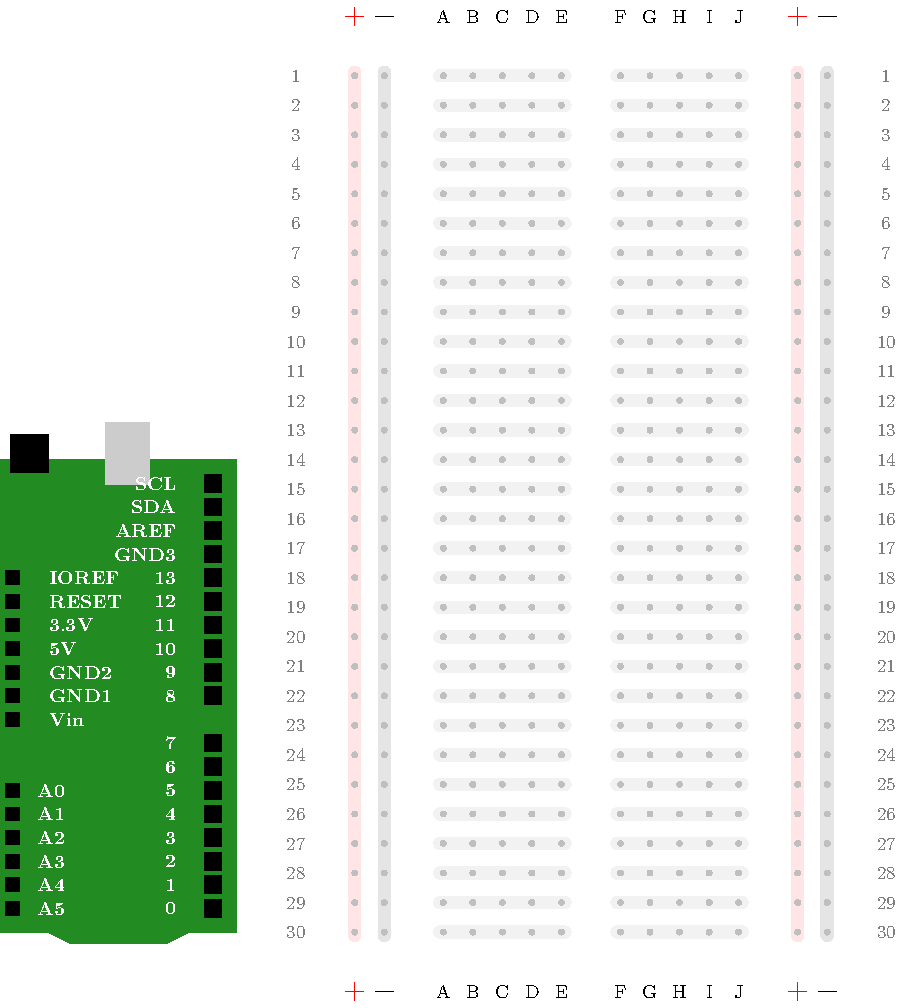
\includegraphics[width=0.9\textwidth]{kuvat/kuva11.pdf}

\begin{tcolorbox}[colback=yellow!10, title={Koodaa!},colbacktitle=orange,breakable]
\begin{solution}
\vspace{18cm}
Tähän tehtävään ei ole malliratkaisua.
\end{solution}
\end{tcolorbox}

\chapter{Lämpötila-anturi ja valoanturi}

\section{Lämpömittari}
\subsection{Lämpötila-anturin käyttöönotto}
\begin{minipage}{0.5\textwidth}
\begin{tcolorbox}[colback=lime!10,title=Tarvikkeet, colbacktitle=green!10,coltitle=black]
\begin{itemize}
    \item Lämpötila-anturi (TMP36) 
    \item Koekytkentälevy
    \item Arduino UNO 
    \item Hyppylankoja
\end{itemize}
\end{tcolorbox}
\end{minipage}
\begin{minipage}{0.5\textwidth}
\begin{tcolorbox}[colback=blue!10,title=Piirin toiminta,colbacktitle=purple!90]
Lämpötila-anturin kytkentä ja käyttö, saadun anturin arvon muuntaminen Celcius-asteiksi.
\tcblower
\begin{center}
\begin{tikzpicture}
\ctikzset{american}
%\draw (0,0) to[R,l=$220\Omega$] (0,-2) to [led] (0,-4);
\draw (-2,0) to[V,a=$5V$] (-2,-4); 
\draw (0,0) to[short] (0,-1.3);
\draw (0,-4) to[short] (0,-2.7);
\draw (0.2,-1.3) -- (-0.2,-1.3);
\draw (-0.2,-1.3)--(-0.2,-2.7);
\draw (-0.2,-2.7)--(0.2,-2.7);
\draw (0.2,-2.7) to[bend right] (0.2,-1.3);
\draw (-0.2,-2)--(-0.5,-2) to[short,-o] (-0.7,-2) node[left] {A0};
\node[text width=0.5] at (0,-2) {T M P};
\draw (-2,0) to[short] (0,0);
\draw (-2,-4) to[short] (0,-4);
\end{tikzpicture}
\end{center}
\end{tcolorbox}
\end{minipage}

\begin{tcolorbox}[colback=red!10,colbacktitle=red,title=HUOM!]
Aina kun rakennat tai muutat piiriä, pidä Arduino irrotettuna tietokoneesta! 
\end{tcolorbox}

\begin{tcolorbox}[title=Lämpötila-anturi,colback=blue!10,colbacktitle=purple!90]
Huomaa, että on merkitystä miten päin lämpötila-anturi kytketään piiriin! 

Jos tasainen sivu on kohti sinua, silloin vasemman puoleisin jalka on käyttöjännite (5V), keskimmäiseltä jalalta (A niin kuin anturi) voidaan lukea tulos ja oikean puoleisin jalka kytketään maahan (GND).

\begin{center}
\begin{tikzpicture}
\node[draw, minimum height=2,color=white,fill=black] (A) at (0,0) {TMP};
\draw[fill=black] (A.north west) to[bend left=70] (A.north east);
\draw[thick] (A.south west)++(0.1,0) --++(0,-0.5) to[short] ++(0,-.5) node[below,left] {5V};
\draw[thick] (A.south) --++(0,-0.5) to[short] ++(0,-.5) node[below] {A};
\draw[thick] (A.south east)++(-0.1,0) --++(0,-0.5) to[short] ++(0,-.5) node[below,right] {GND};
\end{tikzpicture}
\end{center}

Jos kytket anturin väärinpäin, se voi kuumentua. Ole siis tarkkana!
\end{tcolorbox}

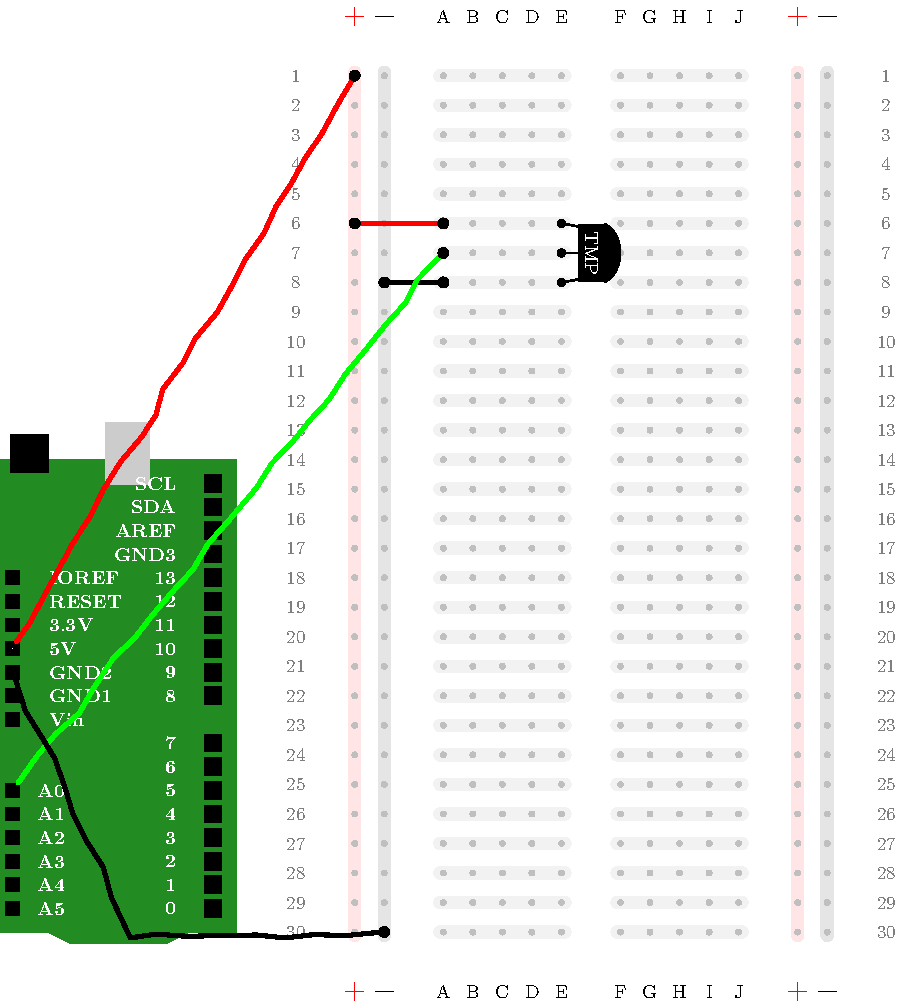
\includegraphics[width=0.8\textwidth]{kuvat/kuva12.pdf}

% \begin{tikzpicture}[scale=0.5]
% \pic[scale=0.2] at (0,0) {myarduino};
% \BREADBOARD(20,30){30};
% \coordinate[right=0.5] (tmp) at (E7);

% \node[draw,minimum height=2,color=white,fill=black] (t1) at (tmp) {\rotatebox[]{-90}{TMP}};
% \draw[fill=black] (t1.north east) to[bend left=70] (t1.south east);
% \draw[thick] (t1.north west)++(0,-0.1)  to[short,-*] (E6);
% \draw[thick] (t1.west) to[short,-*] (E7);
% \draw[thick] (t1.south west)++(0,0.1) to[short,-*] (E8);

% \draw[red,wire] (A6) to[short,*-*] (l-6);
% \draw[black,wire] (A8) to[short,*-*] (lg8);

% \draw[green,wire] (A7) to[short,*-*] (ArA0);

% %\draw[wire,red] (l-10) to[short,*-*] (A10);
% %\draw[wire,black] (lg19) to[short,*-*] (A19);
% \draw[black,wire] (ArGND2) -- ++(4,-9) to[short,-*] (lg30);
% \draw[red,wire] (l-1) to[short,*-o] (Ar5V);
% \end{tikzpicture}

\begin{tcolorbox}[colback=white,title=Vinkkejä Arduinolla koodaamiseen!,colbacktitle=purple!90]
\begin{lstlisting}
// Seuraava rivi kuuluu setup()-funktion sisalle
Serial.begin(9600); // Aloittaa kommunnikoinnin tietokoneen kanssa
// 9600 kertoo kuinka monta bittia sekunnissa lahetetaan.

// Komentoja, joilla voidaan tulostaa
Serial.print(muuttuja); // Tulostetaan muuttujan muuttuja arvo
Serial.print("Teksti:"); // Tulostetaan Teksti: 
Serial.println(muuttuja); // Sama kuin muuttujan tulostus, mutta rivinvaihto lopussa
Serial.print("\n"); // Rivinvaihto manuaalisesti
\end{lstlisting}
\end{tcolorbox}

Nämä tulostetut asiat löytyvät Arduinon "Serial Monitor":sta, eli oikean yläkulman suurennuslasi-kuvakkeen takaa.

\begin{figure}[h!]
    \centering
        \begin{tikzpicture}[remember picture]
\node (fig1) at (0,0)
       {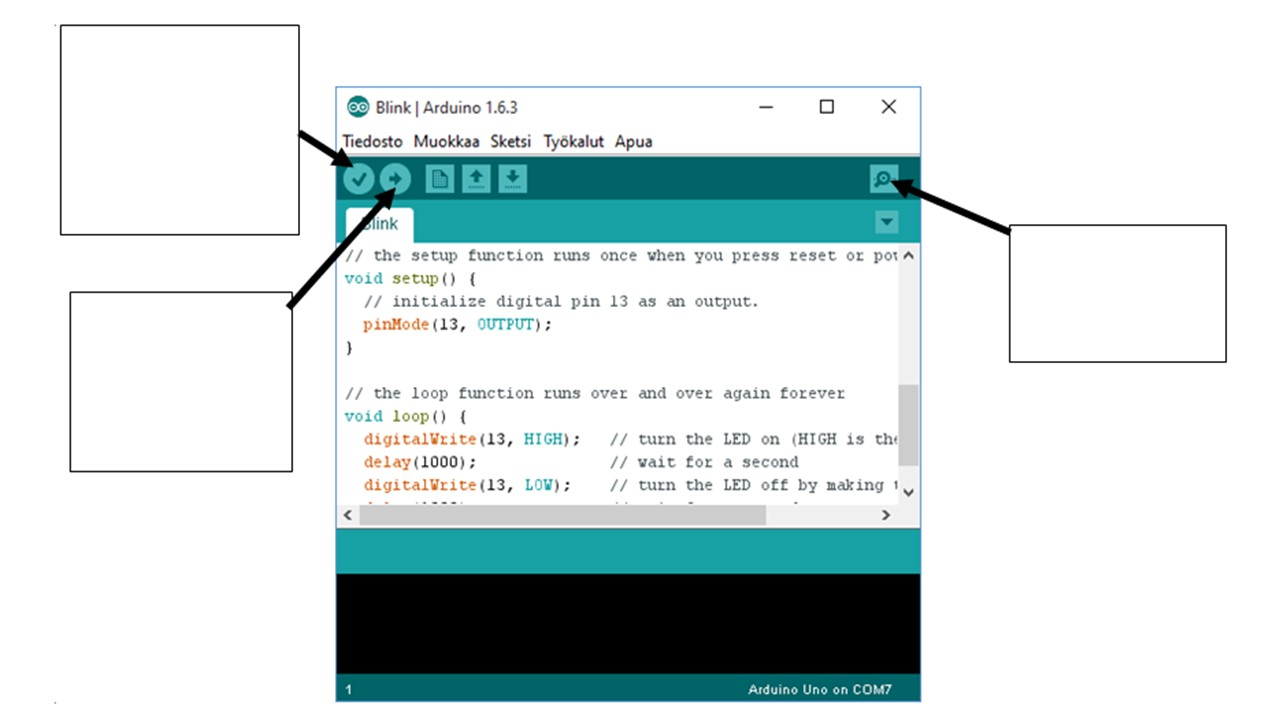
\includegraphics[scale=0.45]{kuvat/ohjelmointiymparisto.jpg}};
\end{tikzpicture}
\begin{tikzpicture}[remember picture, overlay]
       \node [align=left,] at (-5.4,7.7) {\textit{Verify/Tarkista}\\Ohjelma\\tarkistaa\\mutta ei ladata\\Arduinolle };
       \node [align=left,] at (-5.4,4.7) {\textit{Upload/Lataa}\\Ohjelma\\ladataan\\Arduinolle };
       \node [align=left,color=red] at (5.85,5.7) {Avaa sarjaportin\\monitorointi-\\ikkunaan };
\end{tikzpicture}
    %\caption{Arduinon ohjelmointiympäristö ja keskeiset hallinnointi painikkeet. }
    %\label{fig:ohjelmointiymparisto}
\end{figure}

Kopioi alla oleva koodi Arduinoon.
\begin{lstlisting}[numbers=none,showstringspaces=false] 
void setup() {
   Serial.begin(9600);
}

void loop() {
  int sensorVal = analogRead(A0); // Luetaan anturin arvo portista A0
  Serial.print("Anturin arvo: "); // lisataan selitys luvulle
  Serial.print(sensorVal); // ja tulostetaan anturin arvo
  float voltage = (sensorVal/1024.0)*5.0; // Muunna anturin arvo volteiksi
  Serial.print(". Voltteina: "); // Selitys
  Serial.print(voltage);   // Ja tulosta se
  float temp = (voltage-0.5)*100;  // Muunnetaan jannite Celcius-asteiksi
  Serial.print(". Astetta "); // Selitys
  Serial.print(temp); // ja tulostetaan lampotila
  Serial.print(" C\n"); // Celcius-astetta ja vaihdetaan rivia
  delay(1000); // Lisataan odotus, jotta ehditaan lukea tulos
}
\end{lstlisting}

\begin{tcolorbox}[colback=yellow!10, title={Lämpötila},colbacktitle=orange]
Kirjoita ylös saamasi huoneen lämpötila. Esimerkiksi 20.0 astetta.
\end{tcolorbox}

\subsection{LEDien lisääminen}\label{sec:lampo}
\begin{minipage}{0.5\textwidth}
\begin{tcolorbox}[colback=lime!10,title=Tarvikkeet, colbacktitle=green!10,coltitle=black]
\begin{itemize}
    \item Edellisen kohdan piiri rakennettuna
    \item Keltainen ja punainen LED
    \item 2 kappaletta 220$\Omega$ vastuksia:   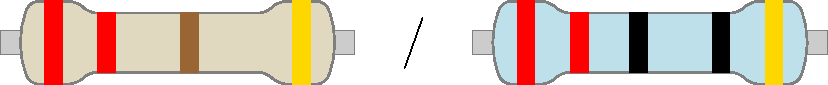
\includegraphics[width=0.5\textwidth]{kuvat/220.pdf}
\end{itemize}
\end{tcolorbox}
\end{minipage}
\begin{minipage}{0.5\textwidth}
\begin{tcolorbox}[colback=blue!10,title=Piirin toiminta,colbacktitle=purple!90]
Lisätään havainnointia varten kaksi LEDiä, joiden avulla saadaan tietää onko huoneessa sopivan lämpöistä, kuumaa vai liian kuumaa.
\tcblower
\begin{center}
\begin{tikzpicture}
\ctikzset{american}
\draw (0,4) to [led,l=punainen,fill=red] (0,2);
\draw (0,2) to[R,a=$220\Omega$] (0,0);
\draw (0,0) -- (0,-0.5) node[ground]{}; 
\draw (-1,4) node[left] {7} to[short,o-] (0,4);

\draw (3,4) to [led,l=keltainen,fill=yellow] (3,2);
\draw (3,2) to[R,a=$220\Omega$] (3,0);
\draw (3,0) -- (3,-0.5) node[ground]{}; 
\draw (2,4) node[left] {6} to[short,o-] (3,4);

\end{tikzpicture}
\end{center}
\end{tcolorbox}
\end{minipage}

\begin{tcolorbox}[colback=red!10,colbacktitle=red,title=HUOM!]
Aina kun rakennat tai muutat piiriä, pidä Arduino irrotettuna tietokoneesta! 
\tcblower
Muista tarkistaa miten päin LEDit kytketään! Tämä löytyy esimerkiksi sivulta \pageref{box:led}.
\end{tcolorbox}

\begin{tcolorbox}[colback=white,title=Vinkkejä Arduinolla koodaamiseen!,colbacktitle=purple!90,breakable]
\begin{lstlisting}
// Halutaan tehda monta asiaa riippuen monesta asiasta
if (ehto) {
    // Mita tehdaan jos ehto patee
} else if (ehto2) {
    // Mita tehdaan jos ehto2 patee
} else if (ehto3) {
   // Naita voit lisata niin monta kuin tarvitset
} else {
    // Ja halutessa voit maaritella myos mita tehdaan muulloin
}

// Erilaisia ehtoja
muuttuja < luku // Muuttujan muuttuja arvo on pienempi kuin annettu luku
muuttuja <= luku // Muuttujan muuttuja arvo on pienempi tai yhta suuri kuin luku
muuttuja > luku // Muuttuja on suurempi kuin luku
// Kaksi ehtoa yhta aikaa
muuttuja >= luku1 && muuttuja < luku2 // Muuttuja on suurempi tai yhtasuuri kuin luku1 JA pienempi kuin luku2
\end{lstlisting}
\end{tcolorbox}

Lisätään LEDit sekä vastukset kuvan mukaisesti.

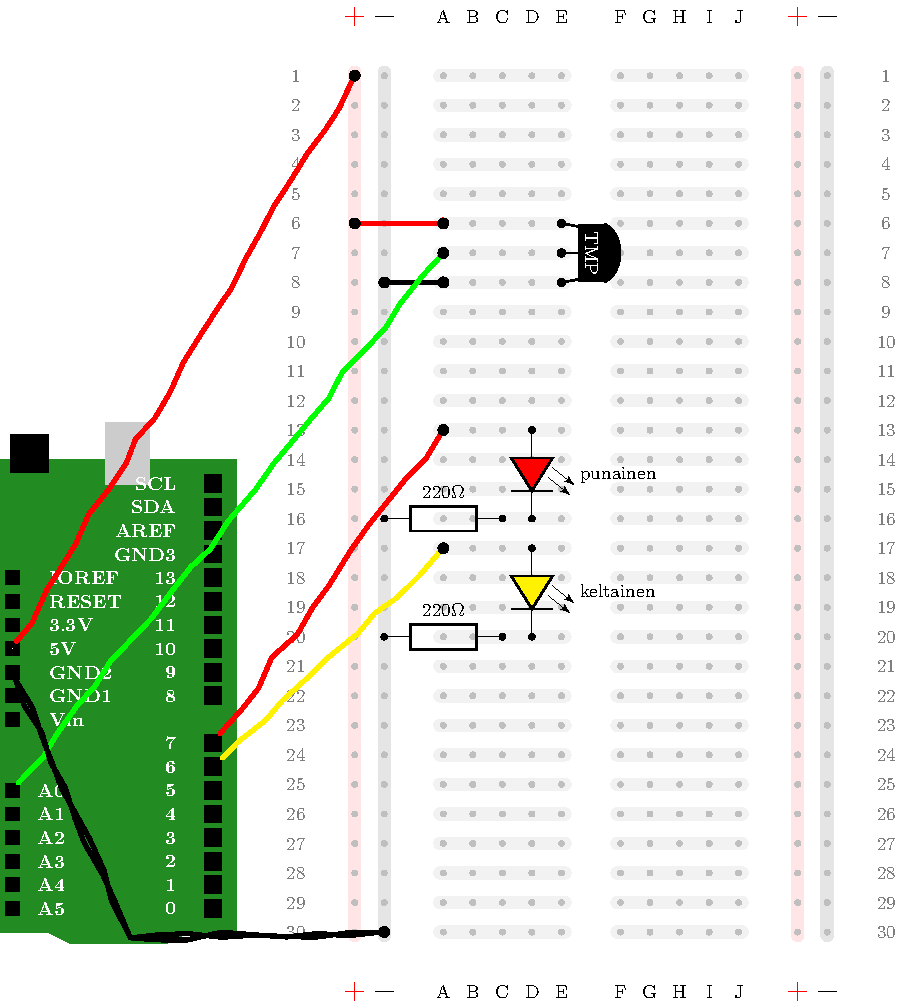
\includegraphics[width=0.8\textwidth]{kuvat/kuva13.pdf}

Lisätään koodiin LEDien ohjaaminen.

\begin{lstlisting}[numbers=none,showstringspaces=false] 
// Lisataan saatu huoneenlampo tahan
const float huoneLamp = 20.0; // Muokkaa lukua edellisen tehtavan mukaiseksi

void setup() {
Serial.begin(9600);
pinMode(7,OUTPUT); // Punainen LED on portissa 7
pinMode(6,OUTPUT); // Keltainen LED on portissa 6
}

void loop() {
  int sensorVal = analogRead(A0); // Luetaan anturin arvo portista A0
  Serial.print("Anturin arvo: "); // lisataan selitys luvulle
  Serial.print(sensorVal); // ja tulostetaan anturin arvo
  float voltage = (sensorVal/1024.0)*5.0; // Muunna anturin arvo volteiksi
  Serial.print(". Voltteina: "); // Selitys
  Serial.print(voltage);   // Ja tulosta se
  float temp = (voltage-0.5)*100;  // Muunnetaan jannite Celcius-asteiksi
  Serial.print(". Astetta "); // Selitys
  Serial.print(temp); // ja tulostetaan lampotila
  Serial.print(" C\n"); // Celcius-astetta ja vaihdetaan rivia

  // Lisataan mita tehdaan jos lampotila nousee tai laskee liikaa
  if (temp <= huoneLamp){
    // Jos huoneen lampo: sytytetaan keltainen LED
    digitalWrite(7,LOW); // Sammutetaan punainen LED tarvittaessa
    digitalWrite(6,HIGH); // Sytytetaan keltainen LED
  }else if(temp>huoneLamp+2 && temp <huoneLamp+4){
    // Lampo on nousemassa: sytytetaan molemmat valot
    digitalWrite(7,HIGH); // Sytytetaan punainen valo
    digitalWrite(6,HIGH); // Sytytetaan keltainen valo
  }else if (temp>huoneLamp+4) {
    // Lampo on noussut liikaa, varoitetaan pelkalla punaisella valolla
    digitalWrite(7,HIGH); // Sytytetaan punainen valo
    digitalWrite(6,LOW); // Sammutetaan keltainen valo
  }
  delay(1000); // Lisataan odotus, etta ehditaan lukea teksti
}
\end{lstlisting}

Nyt, avaa jälleen sarjaportin monitorointi-ikkuna. Ota kevyesti kiinni lämpötila-anturista ja katso missä vaiheessa punainen LED syttyy. Saatko myös keltaisen LEDin sammumaan? 

\begin{tcolorbox}[title=Haaste!,colback=teal!10,colbacktitle=teal!90]
Muuta koodia niin, että jos huoneessa on vähintään 2 astetta kylmempää kuin normaalisti, keltainen valo palaa. Jos huoneessa on taas normaalin lämpöistä, mikään valo ei pala. Jos huoneessa on vähintään 2 astetta lämpimämpää kuin normaalisti, punainen valo palaa.
\end{tcolorbox}

\begin{tcolorbox}[colback=yellow!10, title={Koodaa!},colbacktitle=orange,breakable]
\begin{solution}
\begin{lstlisting}
// Lisataan saatu huoneenlampo tahan
const float huoneLamp = 20.0; // Muokkaa lukua todelliseksi lampotilaksi

void setup() {
Serial.begin(9600);
pinMode(7,OUTPUT); // Punainen LED on portissa 7
pinMode(6,OUTPUT); // Keltainen LED on portissa 6
}

void loop() {
  int sensorVal = analogRead(A0); // Luetaan anturin arvo portista A0
  Serial.print("Anturin arvo: "); // lisataan selitys luvulle
  Serial.print(sensorVal); // ja tulostetaan anturin arvo
  float voltage = (sensorVal/1024.0)*5.0; // Muunna anturin arvo volteiksi
  Serial.print(". Voltteina: "); // Selitys
  Serial.print(voltage);   // Ja tulosta se
  float temp = (voltage-0.5)*100;  // Muunnetaan jannite Celcius-asteiksi
  Serial.print(". Astetta "); // Selitys
  Serial.print(temp); // ja tulostetaan lampotila
  Serial.print(" C\n"); // Celcius-astetta ja vaihdetaan rivia

  // Lisataan mita tehdaan jos lampotin
  if (temp < huoneLamp-2){
    // Huoneessa alkaa olla kylma
    digitalWrite(7,LOW); // Sammutetaan punainen LED tarvittaessa
    digitalWrite(6,HIGH); // Sytytetaan keltainen LED
  }else if(temp>=huoneLamp-2 && temp <huoneLamp+2){
    // Normaalihuoneen lampo
    digitalWrite(7,LOW); // Sytytetaan punainen valo
    digitalWrite(6,LOW); // Sytytetaan keltainen valo
  }else if (temp>huoneLamp+2) {
    // Lampo on noussut liikaa, varoitetaan pelkalla punaisella valolla
    digitalWrite(7,HIGH); // Sytytetaan punainen valo
    digitalWrite(6,LOW); // Sammutetaan keltainen valo
  }
  delay(1000); // Odotetaan, etta ehditaan lukea
}
\end{lstlisting}
Kylmemmäksi muuttumista voi olla vaikeampi havaita, varsinkin jos esimerkiksi ikkunaa ei saa auki, tai ei voida jäähdyttää sormia kylmällä vedellä. Muista, että kädet pitää kuitenkin olla kuivat, jotta voidaan koskea lämpöanturiin!
\end{solution}
\end{tcolorbox}

\clearpage
\section{Valoanturi}
\subsection{Valoanturin käyttöönotto}
\begin{minipage}{0.5\textwidth}
\begin{tcolorbox}[colback=lime!10,title=Tarvikkeet, colbacktitle=green!10,coltitle=black]
\begin{itemize}
    \item Valodiodi 
    \item Koekytkentälevy
    \item Arduino UNO 
    \item Hyppylankoja
    \item Vastus 10k$\Omega$: 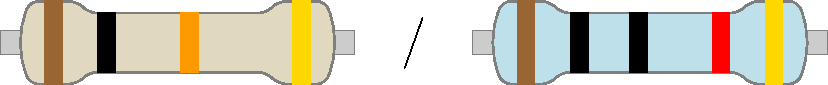
\includegraphics[width=0.5\textwidth]{kuvat/10k.pdf}
\end{itemize}
\end{tcolorbox}
\end{minipage}
\begin{minipage}{0.5\textwidth}
\begin{tcolorbox}[colback=blue!10,title=Piirin toiminta,colbacktitle=purple!90]
Valodiodin käyttö.
\tcblower
\begin{center}
\begin{tikzpicture}
\ctikzset{american}
%\draw (0,0) to[R,l=$220\Omega$] (0,-2) to [led] (0,-4);
\draw (-2,0) to[V,a=$5V$] (-2,-4); 
\draw (0,0) to[photodiode] (0,-2);
\draw (0,-2) to[R=10k$\Omega$] (0,-4);
\draw (0,-2) to[short,*-o] (2,-2) node[right] {A1};
\draw (-2,0) to[short] (0,0);
\draw (-2,-4) to[short] (0,-4);
\end{tikzpicture}
\end{center}
\end{tcolorbox}
\end{minipage}

\begin{tcolorbox}[colback=red!10,colbacktitle=red,title=HUOM!]
Aina kun rakennat tai muutat piiriä, pidä Arduino irrotettuna tietokoneesta! 
\tcblower
Voit jättää vielä edellisen kohdan piirin purkamatta! Sitä tarvitaan seuraavassa työssä. Tämän työn pystyy rakentamaan myös ilman edellisen kohdan piiriä, mutta seuraavassa työssä on käytössä sekä valo- että lämpöanturit.
\end{tcolorbox}

\begin{tcolorbox}[title=Valoanturin kytkeminen,colback=blue!10,colbacktitle=purple!90]
Huomaa, että on merkitystä kummin päin valoanturi kytketään koekytkentälevylle! 

Valoanturissa on kaksi jalkaa, joista toinen on pidempi. Valodiodi näyttää kirkkaalta LEDiltä, mutta siitä puuttuu pyöristetty yläosa, eli yläpinta on tasainen (toisin kuin LEDeillä, joilla se on pyöreä). Piirrosmerkissä nuolet tulevat kohti diodia, eli olemme ottamassa valoa sisään (emmekä lähettämässä sitä ulos kuten LEDin kanssa). 

Valoanturin muovi on toiselta puolelta kaareva, ja toiselta siinä on suora leikkaus, lyhyempi jalka on suoran leikkauksen puolella. Lyhyemmän jalan nimi on katodi ja pidemmän jalan anodi.

Piirrosmerkissä:
\begin{center}
\begin{tikzpicture}
%\node at (-1,0) {anodi};
\draw (0,0) node[left,text width=1.5cm] {anodi\\ pitkä jalka} to[photodiode,o-o] (2,0) node[right,text width=2cm] {katodi\\lyhyt jalka};
\end{tikzpicture}
\end{center}

Valodiodi kytketään myös aina vastuksen kanssa sarjaan, nyt käytössä on 10k$\Omega$ vastus. 
\end{tcolorbox}

\clearpage
Huomaa, että lisäsimme käyttöön myös oikealle puolelle käyttöjännitteen ja maan.

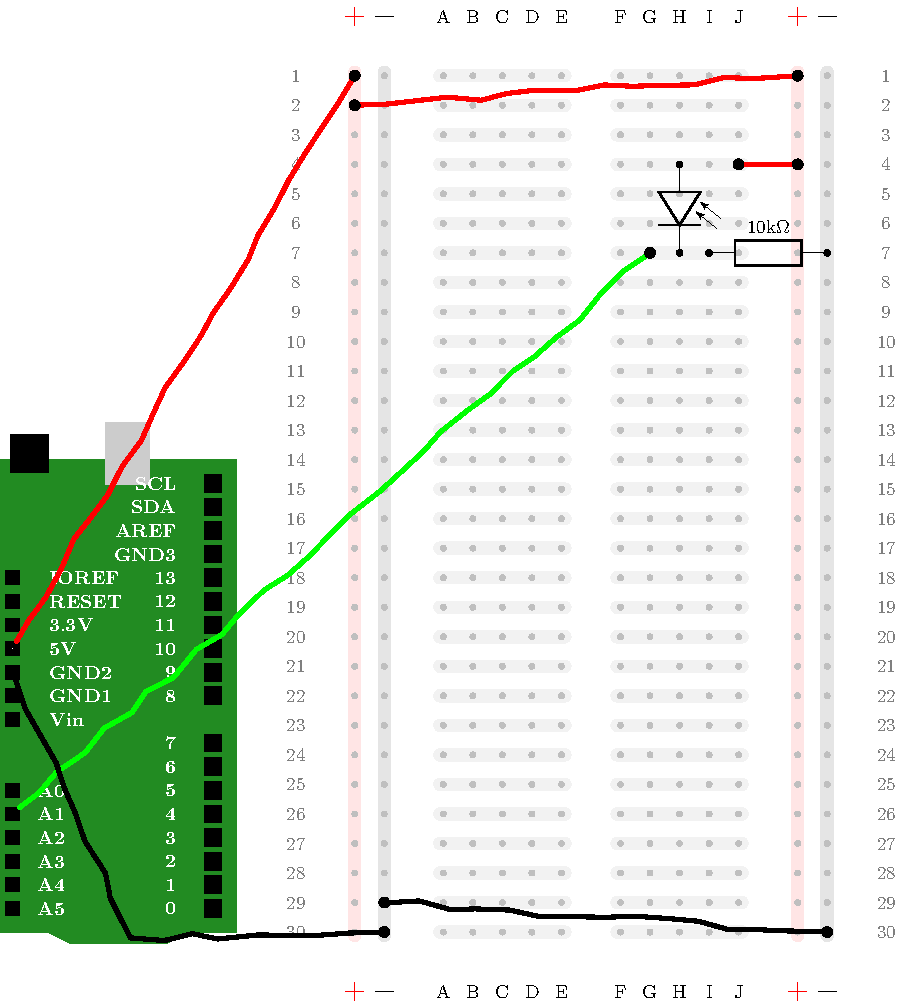
\includegraphics[width=0.8\textwidth]{kuvat/kuva14.pdf}


\begin{lstlisting}[numbers=none,showstringspaces=false]
void setup() {
  Serial.begin(9600);
}

void loop() {
  int valoan = analogRead(A1); // Luetaan anturin arvo portista A1
  Serial.print("Anturin arvo: "); // Selitys
  Serial.println(valoan); // ja tulostetaan se
  delay(1000); // Odotetaan, etta ehditaan lukea
}
\end{lstlisting}

\begin{tcolorbox}[colback=yellow!10, title={Valoanturin arvo},colbacktitle=orange]
Kirjoita ylös saamasi huoneen valoisuutta kuvaava arvo. Esimerkiksi 400.
\end{tcolorbox}

\subsection{LEDien lisääminen}\label{sec:valo}
\begin{minipage}{0.5\textwidth}
\begin{tcolorbox}[colback=lime!10,title=Tarvikkeet, colbacktitle=green!10,coltitle=black]
\begin{itemize}
    \item Edellisen kohdan piiri rakennettuna
    \item Sininen ja vihreä LED
    \item 2 kappaletta 220$\Omega$ vastuksia:   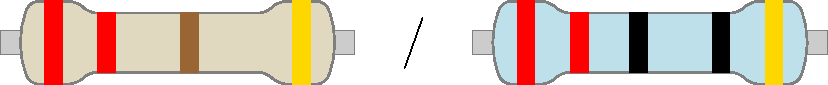
\includegraphics[width=0.5\textwidth]{kuvat/220.pdf}
    \item Taskulamppu tai muu valonlähde
\end{itemize}
\end{tcolorbox}
\end{minipage}
\begin{minipage}{0.5\textwidth}
\begin{tcolorbox}[colback=blue!10,title=Piirin toiminta,colbacktitle=purple!90]
Lisätään havainnointia varten kaksi LEDiä, joilla saadaan tietää onko huoneessa valoisaa vai pimeää.
\tcblower
\begin{center}
\begin{tikzpicture}
\ctikzset{american}
\draw (0,4) to [led,l=vihreä,fill=green] (0,2);
\draw (0,2) to[R,a=$220\Omega$] (0,0);
\draw (0,0) -- (0,-0.5) node[ground]{}; 
\draw (-1,4) node[left] {4} to[short,o-] (0,4);

\draw (3,4) to [led,l=sininen,fill=blue] (3,2);
\draw (3,2) to[R,a=$220\Omega$] (3,0);
\draw (3,0) -- (3,-0.5) node[ground]{}; 
\draw (2,4) node[left] {5} to[short,o-] (3,4);

\end{tikzpicture}
\end{center}
\end{tcolorbox}
\end{minipage}

\begin{tcolorbox}[colback=red!10,colbacktitle=red,title=HUOM!]
Aina kun rakennat tai muutat piiriä, pidä Arduino irrotettuna tietokoneesta! 
\end{tcolorbox}

\clearpage
Lisätään LEDit sekä vastukset kuvan mukaisesti.

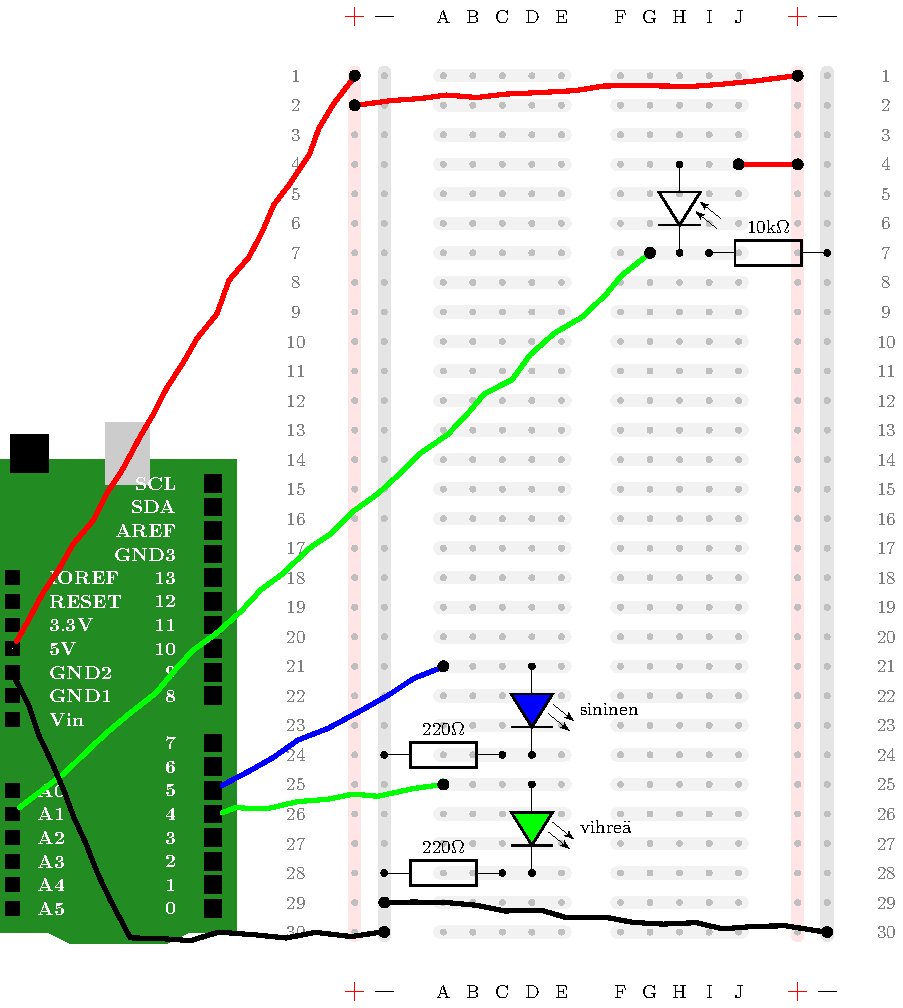
\includegraphics[width=0.9\textwidth]{kuvat/kuva15.pdf}
\clearpage
Lisätään taas LEDit koodiin. 
\begin{lstlisting}[numbers=none]
// Perusvalon aiheuttama lukema
int valo = 400; // Muokkaa arvoksi, jonka sait edellisesta tehtavasta

void setup() {
  Serial.begin(9600);
  pinMode(5,OUTPUT); // Sininen LED
  pinMode(4,OUTPUT); // Vihrea LED
}

void loop() {
  int valoan = analogRead(A1); // Luetaan anturin arvo portista A1
  Serial.print("Anturin arvo: "); // Selitys
  Serial.println(valoan); // ja tulostetaan se

  // Mita tehdaan? 
  if (valoan < valo){
    digitalWrite(5,HIGH); // Sytytetaan sininen valo
    digitalWrite(4,LOW); // Sammutetaan vihrea valo
  } else if (valoan >= valo && valoan < 2*valo) {
    digitalWrite(5,LOW); // Sammutetaan sininen valo
    digitalWrite(4,LOW); // Sammutetaan vihrea valo
  } else if (valoan>=2*valo) {
    digitalWrite(5,LOW); // Sammutetaan sininen valo
    digitalWrite(4,HIGH); // Sytytetaan vihrea valo
  }

  delay(1000); // Odotetaan, etta ehditaan lukea
}
\end{lstlisting}

\begin{tcolorbox}[colback=yellow!10, title={Tutki!},colbacktitle=orange]
Peitä kädellä valoanturi. Kumpi valo syttyy?

Lisää valoa esimerkiksi taskulampulla. Kumpi valo syttyy?

\begin{solution}
Sininen valo syttyy kun on pimeää ja vihreä kun on valoisaa.
\end{solution}
\end{tcolorbox}

\section{Valo- ja lämpöanturit}
\begin{minipage}{0.5\textwidth}
\begin{tcolorbox}[colback=lime!10,title=Tarvikkeet, colbacktitle=green!10,coltitle=black]
\begin{itemize}
    \item Edellisten kahden kohdan piirit (\ref{sec:lampo} ja \ref{sec:valo}) rakennettuna
\end{itemize}
\end{tcolorbox}
\end{minipage}
\begin{minipage}{0.5\textwidth}
\begin{tcolorbox}[colback=blue!10,title=Piirin toiminta,colbacktitle=purple!90]
Yhdistetään valo- ja lämpöanturit.
\end{tcolorbox}
\end{minipage}

\begin{tcolorbox}[colback=red!10,colbacktitle=red,title=HUOM!]
Aina kun rakennat tai muutat piiriä, pidä Arduino irrotettuna tietokoneesta! 
\end{tcolorbox}

Jos sinulla on edelleen jäljellä kohtien \ref{sec:lampo} ja \ref{sec:valo} piirit, sinulla pitäisi olla seuraavan sivun kuvan mukaiset kytkennät. Jos olet kuitenkin purkanut osan piireistä, kokoa se uudelleen kuvan mukaisesti.

\begin{tcolorbox}[title=Haaste!,colback=teal!10,colbacktitle=teal!90]
Suunnittele oma hälytysjärjestelmä, joka reagoi joko valon tai lämmön tai molempien muutoksiin.
\tcblower
Seuraavana on kuva, jossa on yhdistetty molemmat piirit ja sitä seuraa koodi, joka yhdistää jo tekemämme koodit. Voit käyttää sitä pohjana suunnitelmallesi.

\end{tcolorbox}

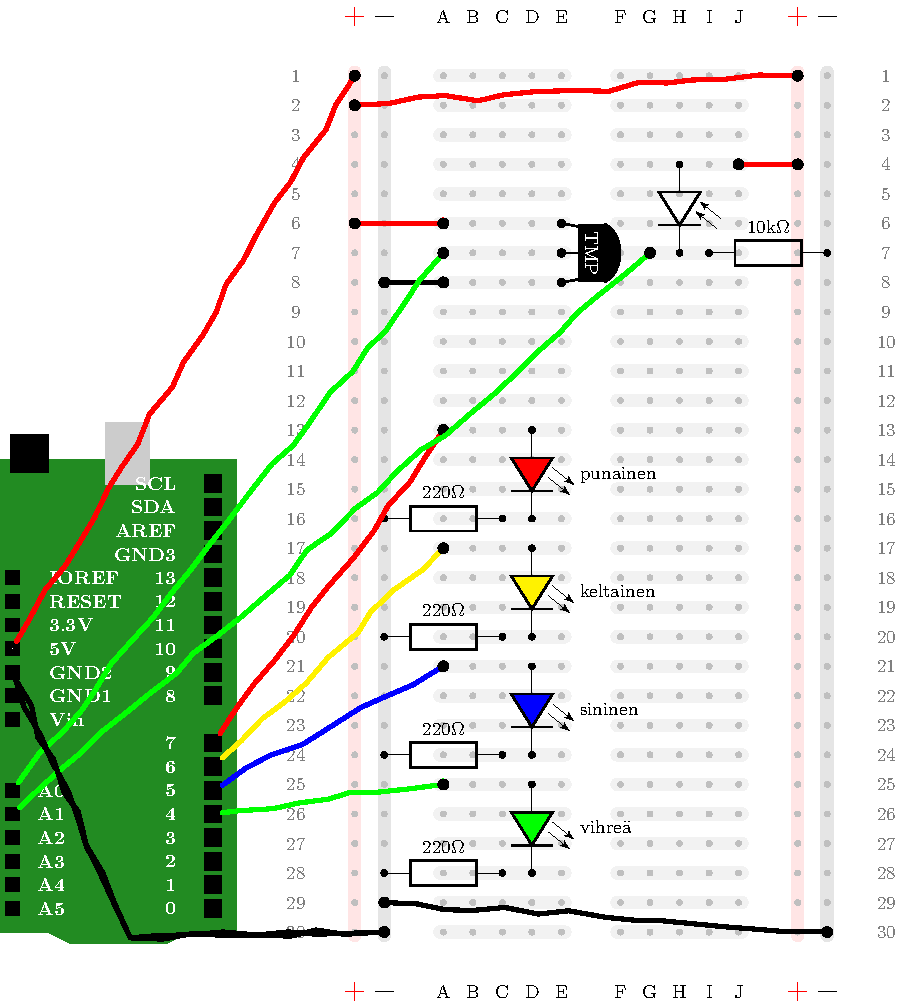
\includegraphics[width=0.95\textwidth]{kuvat/kuva16.pdf}

\begin{lstlisting}[numbers=none]
// Huoneen normaalit lukemat
int valo = 400; // Muokkaa saamaksesi arvoksi
const float huoneLamp = 20.0; // Muokkaa saamaksesi arvoksi

void setup() {
  Serial.begin(9600);
  pinMode(7,OUTPUT); // Punainen LED
  pinMode(6,OUTPUT); // Keltainen LED
  pinMode(5,OUTPUT); // Sininen LED
  pinMode(4,OUTPUT); // Vihrea LED
}

void loop() {
  int valoan = analogRead(A1); // Luetaan valoanturin arvo portista A1
  Serial.print("Valoanturin arvo: "); // Selitys
  Serial.println(valoan); // ja tulostetaan se
  
  int sensorVal = analogRead(A0); // Luetaan anturin arvo portista A0
  Serial.print("Lampotila: "); // lisataan selitys luvulle
  float voltage = (sensorVal/1024.0)*5.0; // Muunna anturin arvo volteiksi
  float temp = (voltage-0.5)*100;  // Muunnetaan jannite Celcius-asteiksi
  Serial.print(temp); // ja tulostetaan lampotila
  Serial.println(" C."); // Celcius-astetta ja vaihdetaan rivia

  // Mita tehdaan? 
  if (valoan < valo){
    digitalWrite(5,HIGH); // Sytytetaan sininen valo
    digitalWrite(4,LOW); // Sammutetaan vihrea valo
  } else if (valoan >= valo && valoan < 2*valo) {
    digitalWrite(5,LOW); // Sammutetaan sininen valo
    digitalWrite(4,LOW); // Sammutetaan vihrea valo
  } else if (valoan>=2*valo) {
    digitalWrite(5,LOW); // Sammutetaan sininen valo
    digitalWrite(4,HIGH); // Sytytetaan vihrea valo
  }

  if (temp < huoneLamp-2){
    // Huoneessa alkaa olla kylma
    digitalWrite(7,LOW); // Sammutetaan punainen LED tarvittaessa
    digitalWrite(6,HIGH); // Sytytetaan keltainen LED
  }else if(temp>=huoneLamp-2 && temp <huoneLamp+2){
    // Normaalihuoneen lampo
    digitalWrite(7,LOW); // Sytytetaan punainen valo
    digitalWrite(6,LOW); // Sytytetaan keltainen valo
  }else if (temp>huoneLamp+2) {
    // Lampo on noussut liikaa, varoitetaan pelkalla punaisella valolla
    digitalWrite(7,HIGH); // Sytytetaan punainen valo
    digitalWrite(6,LOW); // Sammutetaan keltainen valo
  }
 
  delay(1000); // Odotetaan, etta ehditaan lukea
}
\end{lstlisting}



\begin{tcolorbox}[colback=yellow!10, title={Koodaa!},colbacktitle=orange,breakable]
\vspace{15cm}
\begin{solution}
%\vspace{15cm}

Tähän tehtävään ei ole malliratkaisua
\end{solution}
\end{tcolorbox}
\chapter{LCD-näyttö}
\section{LCD-näytön kytkentä}\label{sec:lcd}

\begin{minipage}{0.5\textwidth}
\begin{tcolorbox}[colback=lime!10,title=Tarvikkeet, colbacktitle=green!10,coltitle=black]
\begin{itemize}
    \item Koekytkentälevy
    \item Arduino UNO 
    \item Potentiometri
    \item Hyppylankoja
    \item Vastus 220$\Omega$: 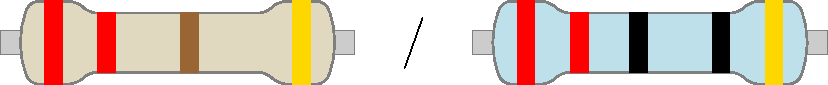
\includegraphics[width=0.5\textwidth]{kuvat/220.pdf}
    \item LCD-näyttö
\end{itemize}
\end{tcolorbox}
\end{minipage}
\begin{minipage}{0.5\textwidth}
\begin{tcolorbox}[colback=blue!10,title=Piirin toiminta,colbacktitle=purple!90]
Tutustutaan LCD-näytön käyttämiseen. Kirjoitetaan oma viesti näytölle. Potentiometrin käyttäminen ja sen avulla näytön kirkkauden säätäminen.
\end{tcolorbox}
\end{minipage}

\begin{tcolorbox}[colback=red!10,colbacktitle=red,title=HUOM!]
Aina kun rakennat tai muutat piiriä, pidä Arduino irrotettuna tietokoneesta! 
\tcblower
Huomaa, että LCD-näytön kytkemiseen tarvitaan useita hyppylankoja ja se vaatii tarkkuutta!
\end{tcolorbox}

\begin{tcolorbox}[title=Potentiometrin kytkeminen,colback=blue!10,colbacktitle=purple!90]
Potentiometri on säädettävä vastus, jossa on kolme jalkaa, kaksi toisella puolella ja yksi toisella. Se kytketään uran ylitse, niin että kaksi jaloista ovat toisella puolella ja yksi toisella puolella. Potentiometrin mukana tulee valkoinen säätönuppi, jolla vastuksen arvoa voidaan säädellä pyörittämällä nuppia. 

\begin{minipage}{0.8\textwidth}
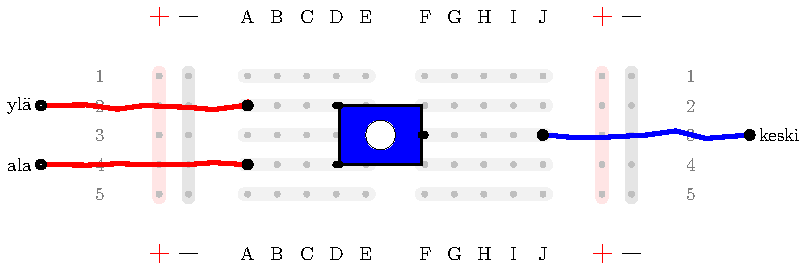
\includegraphics[width=\textwidth]{kuvat/kuva17.pdf}
\end{minipage}%
\begin{minipage}{0.2\textwidth}
Piirrustusmerkki:

\begin{circuitikz} 
\draw (0,0) node[left] {ylä} to[american potentiometer,n=mypot] ++(0,-2) node[right] {ala} (mypot.wiper) to[short] ++(1,0) node[above] {keski};
\end{circuitikz}
\end{minipage}

Mitattaessa vastuksen arvoa välillä ylä-ala, vastuksen arvo pysyy vakiona. Jos taas käytetään vastusta välillä ylä-keski tai keski-ala, vastuksen arvoa voidaan muuttaa pyörittämällä säätönuppia.
\end{tcolorbox}

\clearpage
Kytketään näyttöön tarvittavat asiat osissa koekytkentälevylle. Ole tarkkana rivien kanssa!

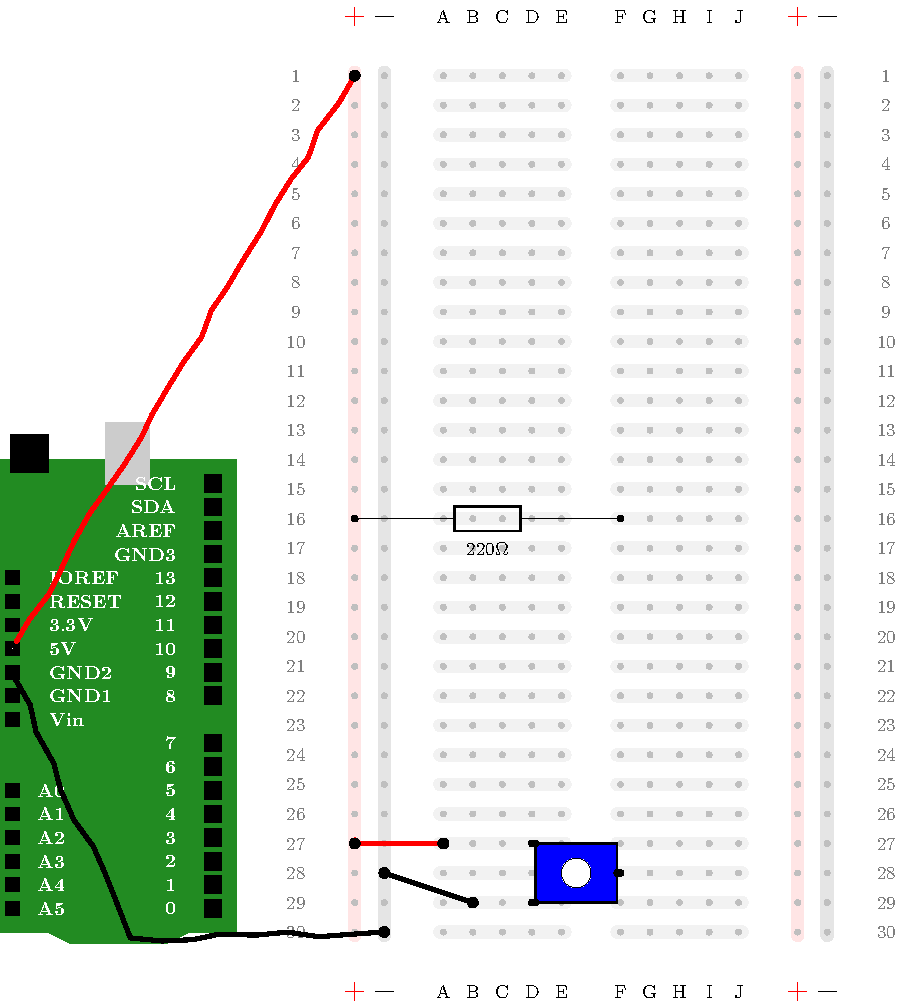
\includegraphics[width=0.95\textwidth]{kuvat/kuva19.pdf}

Kytketään ensin potentiometri pisteisiin D27, D29 ja F28. Kytke rivi 27 vasen puoli käyttöjännitteeseen (punainen + rivi) ja rivi 29 vasen puoli maahan. Kytketään sitten vastus käyttöjännitteen (punainen +, vasen laita) ja F16 välille. Muista myös kytkeä käyttöjännite vasemmalle + riville ja maa vasemmalle - riville.
%%%%%%%%%%%%%%%%%%%%%%%%%

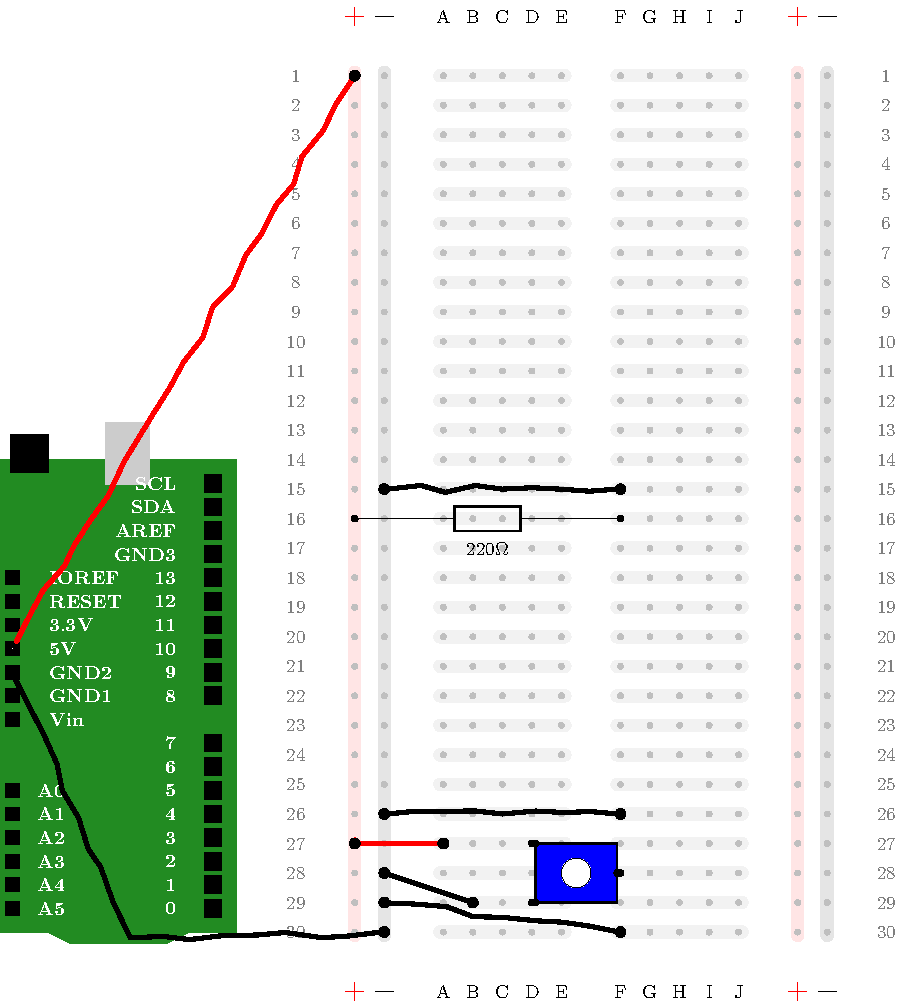
\includegraphics[width=0.95\textwidth]{kuvat/kuva20.pdf}

Kytketään sitten maat: rivi 26 oikea puoli maahan, rivi 30 oikea puoli maahan, ja rivi 15 oikea puoli maahan.

%%%%%%%%%%%%%%%%%%%

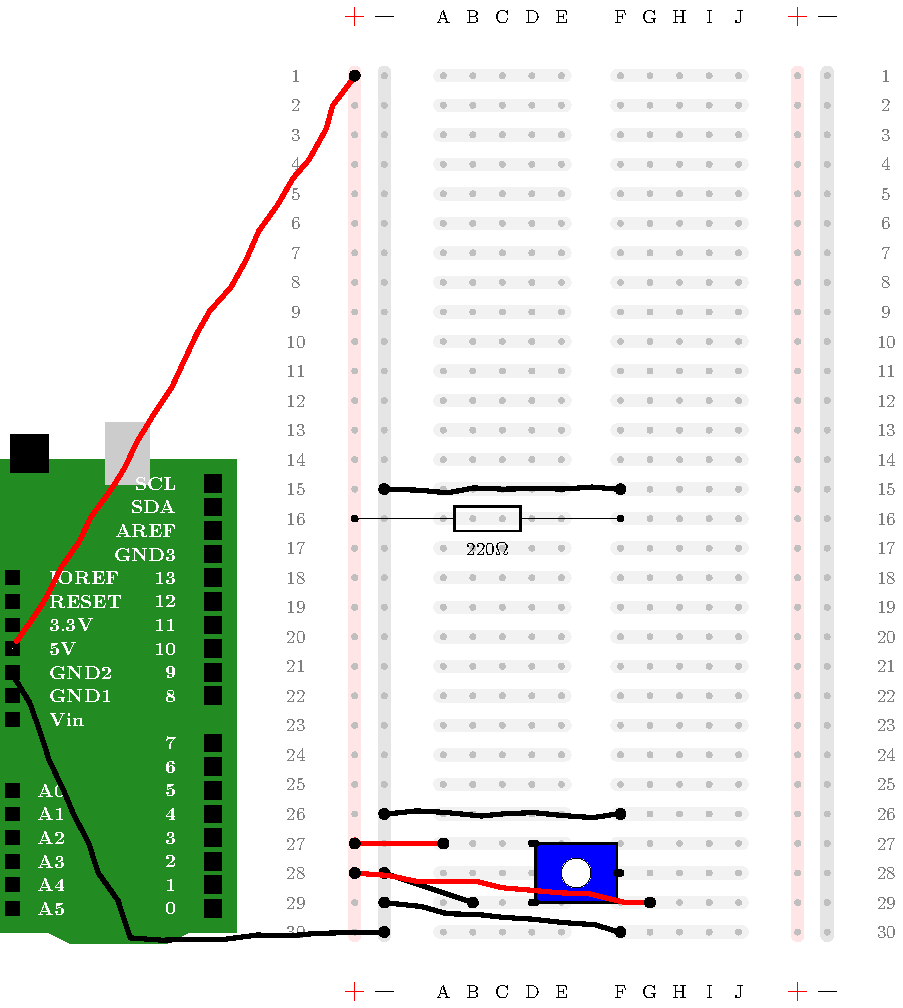
\includegraphics[width=0.95\textwidth]{kuvat/kuva21.pdf}

Kytketään sitten loput käyttöjännitteet: rivi 29 oikea puoli vasempaan plus-riviin (5V). 

%%%%%%%%%%%%%%%%%%

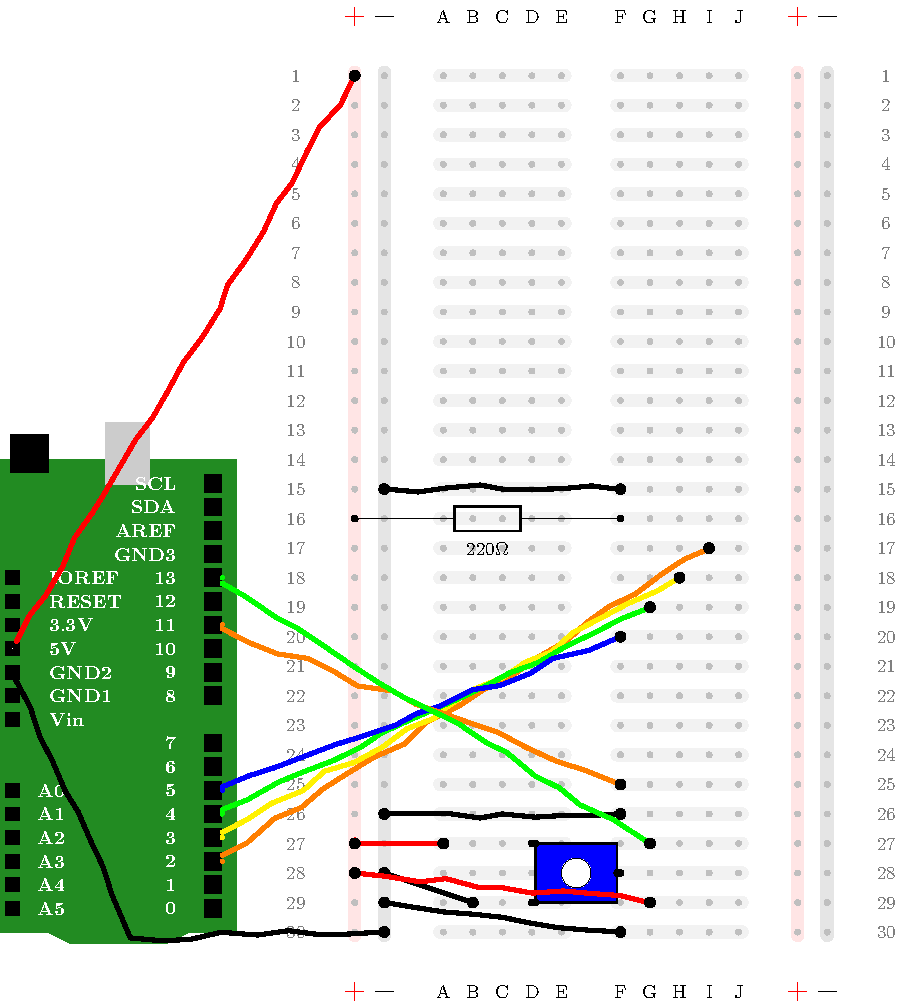
\includegraphics[width=0.95\textwidth]{kuvat/kuva22.pdf}

Kytketään Arduinon puolelta pinni 2 oikealle riville 17, pinni 3 oikealle riville 18, pinni 4 oikealle riville 19 ja pinni 5 oikealle riville 20. Lisäksi pinni 11 oikealle riville 25 ja pinni 13 oikealle riville 27. 

%%%%%%%%%%%%%%%%

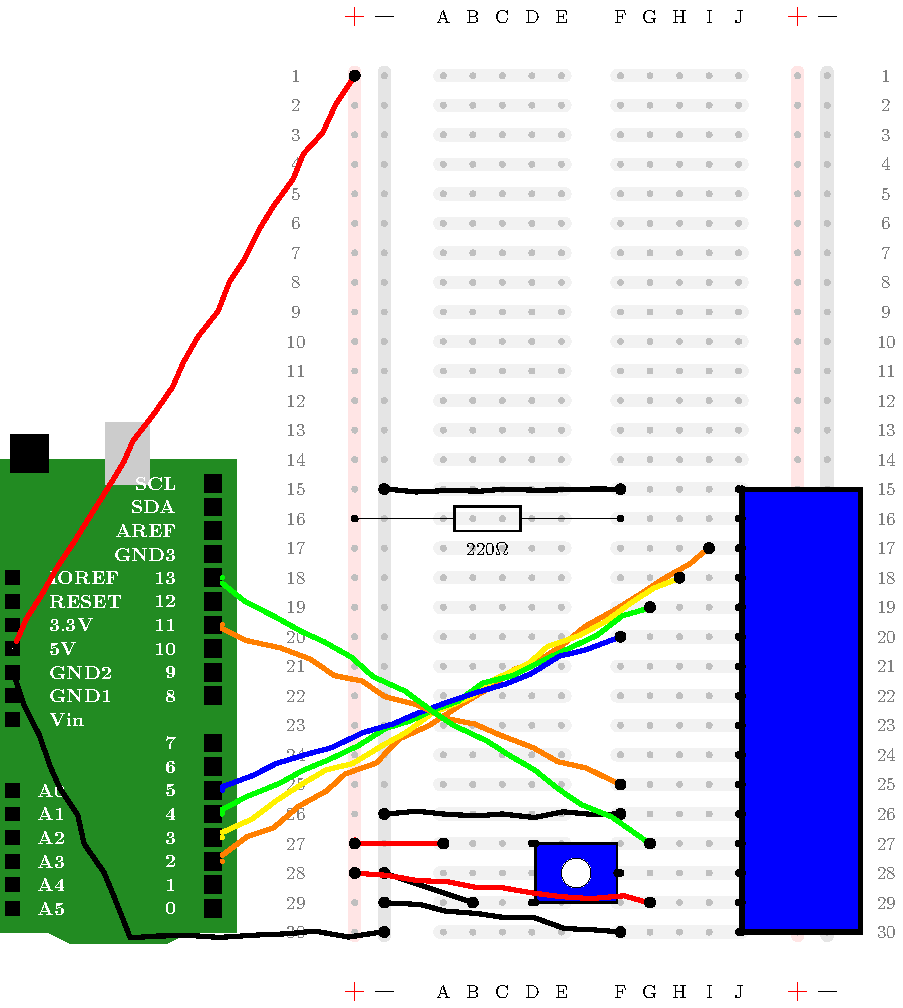
\includegraphics[width=0.9\textwidth]{kuvat/kuva23.pdf} \label{fig:lcd}

Viimeiseksi lisään LCD-näyttö kiinni pinneihin J15-J30.

\clearpage
Seuraavaksi koodataan Arduinolla näytölle tekstiä kahteen riviin. LCD-näytöllä on kaksi riviä, joiden pituus on 16 merkkiä riviä kohti. 

\begin{tcolorbox}[colback=white,title=Vinkkejä Arduinolla koodaamiseen!,colbacktitle=purple!90]
\begin{lstlisting}
// LCD-nayton kayttaminen onnistuu kirjaston avulla:
#include <LiquidCrystal.h> // Lisataan kirjasto 
// Arduinolle pitaa kertoa missa pinneissa naytto on kiinni:
LiquidCrystal lcd(13,11,5,4,3,2); // Digital Pinnit joissa kiinni

// Taman jalkeen naytolle voidaan tulostaa:
lcd.print("Viesti.");
// Naytto voidaan tyhjentaa
lcd.clear();
// Osoittimen paikkaa voidaan siirtaa:
lcd.setCursor(luku1, luku2);
// luku1 kertoo kuinka mones nayton osa (0-15)
// luku2 kertoo kumpi rivi, 0 = ylempi, 1 = alempi
\end{lstlisting}
\end{tcolorbox}

Kopioi koodi ja testaa, että saat näytölle näkyviin tekstin "Tervetuloa (Nimesi)". Jos näytöllä ei näy mitään, niin kokeile pyörittää potentiometria nupin avulla. Potentiometri säätää näytön kirkkautta. 

\begin{lstlisting}[numbers=none]
#include <LiquidCrystal.h> // Lisataan kirjasto 
LiquidCrystal lcd(13,11,5,4,3,2); // Digital Pinnit joissa kiinni

void setup() {
  lcd.begin(16,2); // Kaynnistetaan naytto
  lcd.print("Tervetuloa"); // Kirjoitetaan ekalle riville
}

void loop() {
  lcd.setCursor(0,1); // Siirrytaan toiselle riville
  lcd.print("Nimi"); // Kirjoita oma nimesi tahan
}
\end{lstlisting}

\clearpage
Seuraavaksi testataan, miten saadaan aikaan liikkuva teksti toiselle riville.

\begin{lstlisting}[numbers=none]
#include <LiquidCrystal.h> // Lisataan kirjasto 
LiquidCrystal lcd(13,11,5,4,3,2); // Digital Pinnit joissa kiinni

char * viesti = "Tanaan on ohjelmointipaiva.";

void setup() {
  lcd.begin(16,2);
  lcd.print("Tervetuloa");
}

void loop() {
  // Naytolle mahtuu 16 merkkia per rivi
  for (int letter = 0; letter <= strlen(viesti); letter++) {
    naytaViesti(0,letter);
  }
}

void naytaViesti(int printStart, int startLetter) {
  lcd.setCursor(printStart,1);
  for (int letter = startLetter; letter<=startLetter+15; letter++) {
    if (letter <=strlen(viesti)-1){
      lcd.print(viesti[letter]);
    } else {
      lcd.print(" ");
    }
  }
  lcd.print(" ");
  delay(300); // Lisataan viive, etta ehdimme lukea
}
\end{lstlisting}
Nyt alemmalla rivillä pitäisi liikkua määrittelemänne viesti! Voit muokata viestin liikkumisnopeutta muokkaamalla viivettä. Muokkaa koodia oman tervehdysten lähettämiseen!

\begin{tcolorbox}[colback=yellow!10, title={Koodaa!},colbacktitle=orange,breakable]
\begin{solution}
\begin{lstlisting}
#include <LiquidCrystal.h> // Lisataan kirjasto 
LiquidCrystal lcd(13,11,5,4,3,2); // Digital Pinnit joissa kiinni

// Tata muokkaamalla saadaan eri liikkuvia viesteja. 
char * viesti = "Tanaan on ohjelmointipaiva.";

void setup() {
  lcd.begin(16,2);
  lcd.print("Tervetuloa"); // Tata muokkaamalla ylarivi pysyy samana
}

void loop() {
  // Naytolle mahtuu 16 merkkia per rivi
  for (int letter = 0; letter <= strlen(viesti); letter++) {
    naytaViesti(0,letter);
  }
}

void naytaViesti(int printStart, int startLetter) {
  lcd.setCursor(printStart,1);
  for (int letter = startLetter; letter<=startLetter+15; letter++) {
    if (letter <=strlen(viesti)-1){
      lcd.print(viesti[letter]);
    } else {
      lcd.print(" ");
    }
  }
  lcd.print(" ");
  delay(300); // Lisataan viive, etta ehdimme lukea
}
\end{lstlisting}
\end{solution}
\end{tcolorbox}

\clearpage
\section{Lämpötilan mittaaminen ja näyttäminen näytöllä}
\begin{minipage}{0.5\textwidth}
\begin{tcolorbox}[colback=lime!10,title=Tarvikkeet, colbacktitle=green!10,coltitle=black]
\begin{itemize}
    \item Edellisen kohdan piiri rakennettuna
    \item Lämpötila-anturi (TMP36)
    \item Hyppylankoja
\end{itemize}
\end{tcolorbox}
\end{minipage}
\begin{minipage}{0.5\textwidth}
\begin{tcolorbox}[colback=blue!10,title=Piirin toiminta,colbacktitle=purple!90]
Mitataan huoneen lämpötila ja tulostetaan se LCD-näytölle.
\end{tcolorbox}
\end{minipage}

\begin{tcolorbox}[colback=red!10,colbacktitle=red,title=HUOM!]
Aina kun rakennat tai muutat piiriä, pidä Arduino irrotettuna tietokoneesta! 
\end{tcolorbox}

Lisätään lämpötila-anturi piiriin kuvan mukaisesti ja liitetään sen mittaus porttiin A0. 


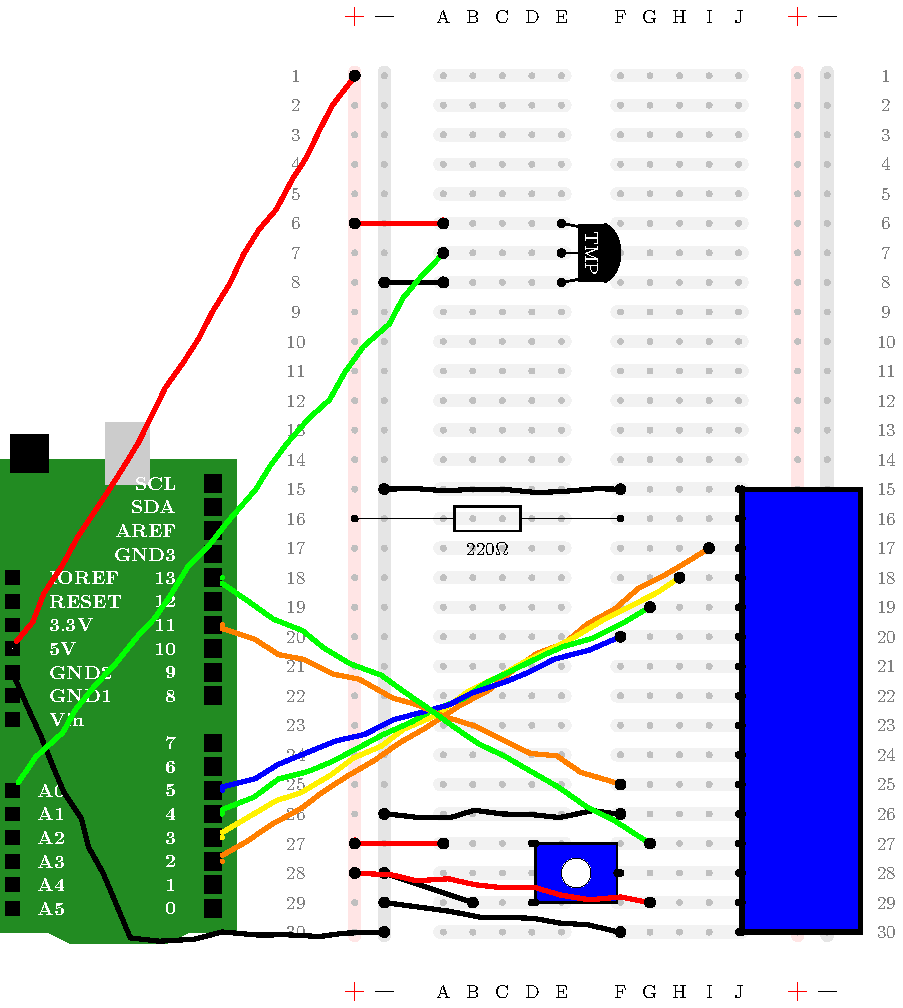
\includegraphics[width=0.8\textwidth]{kuvat/kuva24.pdf}

Kuten jo aiemmin, kun mittasimme lämpötilaa, voimme tehdä samoin nyt ja tulostaa lämpötilan serial portin sijaan näytölle.

\begin{lstlisting}[numbers=none]
#include <LiquidCrystal.h> // Lisataan kirjasto 
LiquidCrystal lcd(13,11,5,4,3,2); // Digital Pinnit joissa kiinni

void setup() {
  lcd.begin(16,2); // Aloitetaan kaytto
  lcd.print("Lampotila"); // Tulostetaan ensimmaiselle riville lampotila
}

void loop() {
  // Mitataan lampotila ja muunnetaan se asteiksi
  int sensorVal = analogRead(A0);
  float voltage = (sensorVal/1024.0)*5.0;
  float temp = (voltage-0.5)*100;
  // Ja tulostetaan se
  lcd.setCursor(0,1);
  lcd.print(temp);
  // Odotetaan arvojen paivittamisen valilla, etta luvut eivat hypi
  delay(1000);  
}
\end{lstlisting}
%%%%%%%%%%%%%%%%%%%%%%
\clearpage
\section{LCD-näyttö ja vaihtuvat viestit}
\begin{minipage}{0.5\textwidth}
\begin{tcolorbox}[colback=lime!10,title=Tarvikkeet, colbacktitle=green!10,coltitle=black]
\begin{itemize}
    \item Edellisen kohdan piiri rakennettuna
    \item Kaltevuusanturi
    \item Vastus 10k$\Omega$: 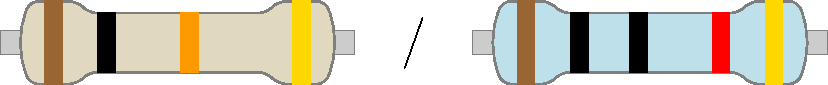
\includegraphics[width=0.5\textwidth]{kuvat/10k.pdf}
\end{itemize}
\end{tcolorbox}
\end{minipage}
\begin{minipage}{0.5\textwidth}
\begin{tcolorbox}[colback=blue!10,title=Piirin toiminta,colbacktitle=purple!90]
Vaihdetaan LCD-näytön tekstiä kun havaitaan, että piiriä on kallistettu.
\end{tcolorbox}
\end{minipage}

\begin{tcolorbox}[colback=red!10,colbacktitle=red,title=HUOM!]
Aina kun rakennat tai muutat piiriä, pidä Arduino irrotettuna tietokoneesta! 
\end{tcolorbox}

\begin{tcolorbox}[title=Kaltevuusanturin kytkeminen,colback=blue!10,colbacktitle=purple!90]
Kaltevuusanturissa on neljä jalkaa, ja se vaatii kaksi riviä koekytkentälevystä. Kaltevuusanturi näyttää suorakulmaiselta laatikolta, jonka lähes neliönmuotoisella päällä lukee "UP" ja on nuoli ylös. Tämä rivi, jolla nuoli on, kytketään käyttöjännitteeseen ja toinen rivi kytketään vastuksen kautta maahan. Mittaustulos voidaan lukea samalta riviltä mille vastus on kytketty.  


\begin{tikzpicture}[scale=0.5]
\BREADBOARD (0,0) {5};
\draw[thick,fill=black] (D3.east) rectangle (E4.west) node[pos=0.5,color=white] {UP};
\draw (D3.east) to[short,*-*] (D3);
\draw (D4.east) to[short,*-*] (D4);
\draw (E3.west) to[short,*-*] (E3);
\draw (E4.west) to[short,*-*] (E4);

\draw[wire,red] (A3) to[short,*-o] ++(-7,0) node[left,black] {Käyttöjännite};
\draw[wire,blue] (A4) to[short,*-o] ++(-7,0) node[left,black] {Mittaus};

\end{tikzpicture}
\end{tcolorbox}

\begin{tcolorbox}[colback=white,title=Vinkkejä Arduinolla koodaamiseen!,colbacktitle=purple!90,breakable]
\begin{lstlisting}
// Satunnaisen luvun arpominen
int satunnainen = random(luku); //  satunnainen kokonaisluku valilta 0-annettu luku
// Ehtolause: ei yhta suuri kuin
luku1 != luku2
// Vaihtoehtoisia tapauksia
switch(luku) {
    case 0:
    // mita tehdaan jos luku on nolla
    break; // lopetetaan
    case 1: 
    // kun luku on 1
    break;
    // Lisaa case numero: riveja niin monta yhteensa kuin lukusi on ja kerro mita tehdaan, ja poistu sen jalkeen ulompaan koodiin break:n avulla
}
\end{lstlisting}
\end{tcolorbox}


Kytketään kaltevuusanturi ja vastus piiriin ja mitataan anturin antamaa arvoa pinnin 6 avulla. 

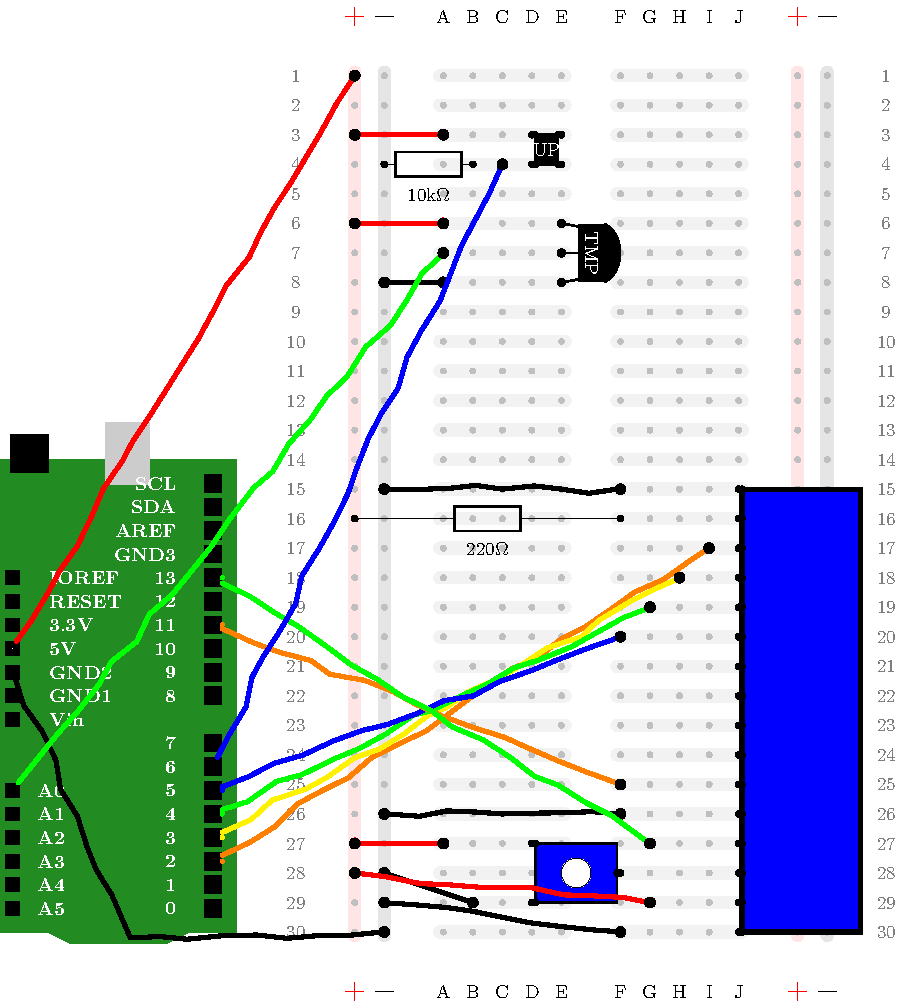
\includegraphics[width=0.8\textwidth]{kuvat/kuva25.pdf}


\clearpage
Lisätään koodiin kaltevuusanturin lukeminen ja koodataan muutama eri viesti näytöllä näytettäväksi.

\begin{lstlisting}[numbers=none]
#include <LiquidCrystal.h> // Lisataan kirjasto 
LiquidCrystal lcd(13,11,5,4,3,2); // Digital Pinnit joissa kiinni

int switchState = 0;
int prevSwitchState = 0;
int reply;

void setup() {
  lcd.begin(16,2);
  pinMode(6, INPUT); // Kaltevuusanturi pinnissa 6
  lcd.print("Hetken miete");
}

void loop() {
  // Luetaan kaltevuusanturin tila
  switchState = digitalRead(6);
  // Jos tila ei ole sama kuin edellinen tila, tehdaan asioita
  if (switchState != prevSwitchState) {
    if (switchState == LOW) {
      // Arvotaan mita naytetaan
      reply = random(4);
      // Tyhjennetaan naytto
      lcd.clear();
      // Asetetaan kursori ensimmaisen rivin alkuun
      lcd.setCursor(0,0);
      // Annetaan eri tapaukset ja mita tehdaan milloinkin
      switch(reply){
        case 0:
        lcd.print("Kytke ne");
        lcd.setCursor(0,1);
        lcd.print("sarjaan!");
        break;
        case 1:
        lcd.print("Kytke ne");
        lcd.setCursor(0,1);
        lcd.print("rinnan!");
        break;
        case 2:
        lcd.print("LEDit");
        lcd.setCursor(0,1);
        lcd.print("palaa!");
        break;
        case 3:
        lcd.print("Lampotila");
        lcd.setCursor(0,1);
        int sensorVal = analogRead(A0);
        float volt = (sensorVal/1024.0)*5.0;
        float temp = (volt-0.5)*100;
        lcd.print(temp);
        break;
      }
    }
  } 
  // Viimekseksi tallennetaan edelliseksi tilaksi nykyinen tila
  prevSwitchState = switchState;
}
\end{lstlisting}

Testaa toiminta nostamalla sitä. Heiluta varovasti koekytkentälevyä, niin että viestit vaihtuvat näytöllä.

\begin{tcolorbox}[title=Haaste!,colback=teal!10,colbacktitle=teal!90]
Muuta koodia niin, että saat aikaa mystisen kasipallon! Eli, koodaa 8 eri vastausta kysymyksiin, jotka saat esiin ravistamalla kevyesti koekytkentälevyä.
\end{tcolorbox}

\begin{tcolorbox}[colback=yellow!10, title={Koodaa!},colbacktitle=orange,breakable]
\begin{solution}
\begin{lstlisting}
#include <LiquidCrystal.h> // Lisataan kirjasto 
LiquidCrystal lcd(13,11,5,4,3,2); // Digital Pinnit joissa kiinni

int switchState = 0;
int prevSwitchState = 0;
int reply;

void setup() {
  lcd.begin(16,2);
  pinMode(6, INPUT); // Kaltevuusanturi pinnissa 6
  lcd.print("Mystinen");
  lcd.setCursor(0,1);
  lcd.print("Kasipallo!");
}

void loop() {
  // Luetaan kaltevuusanturin tila
  switchState = digitalRead(6);
  // Jos tila ei ole sama kuin edellinen tila, tehdaan asioita
  if (switchState != prevSwitchState) {
    if (switchState == LOW) {
      // Arvotaan mita naytetaan
      reply = random(8);
      switch(reply){
        case 0:
        lcd.clear();
        lcd.setCursor(0,0);
        lcd.print("Tietokone sanoo");
        lcd.setCursor(0,1);
        lcd.print("ei.");
        break;
        case 1:
        lcd.clear();
        lcd.setCursor(0,0);
        lcd.print("Tottakai!");
        break;
        case 2:
        lcd.clear();
        lcd.setCursor(0,0);
        lcd.print("Ei missaan");
        lcd.setCursor(0,1);
        lcd.print("nimessa");
        break;
        case 3:
        lcd.clear();
        lcd.setCursor(0,0);
        lcd.print("Kuuma!");
        break;
        case 4:
        lcd.clear();
        lcd.setCursor(0,0);
        lcd.print("Kylma!");
        break;
        case 5:
        lcd.clear();
        lcd.setCursor(0,0);
        lcd.print("Mahdollisesti!");
        break;
        case 6:
        lcd.clear();
        lcd.setCursor(0,1);
        lcd.print("Huomenna!");
        case 7:
        lcd.clear();
        lcd.setCursor(0,0);
        lcd.print("Lampotila");
        lcd.setCursor(0,1);
        int sensorVal = analogRead(A0);
        float volt = (sensorVal/1024.0)*5.0;
        float temp = (volt-0.5)*100;
        lcd.print(temp);
        break;
      }
    }
  } 
  // Viimekseksi tallennetaan edelliseksi tilaksi nykyinen tila
  prevSwitchState = switchState;
}
\end{lstlisting}
Keskustelua voi nostaa esimerkiksi siitä, kuinka satunnainen random() oikeastaan on. 

Kannattaa muistaa myös, että Arduinossa on piirissä reset-nappula tietokone-liitännen vieressä, jos haluat palauttaa koodin takaisin alkupisteeseen.
\end{solution}
\end{tcolorbox}

\appendix
\chapter{Komponenttipankki}
Tässä osuudessa on kerätty yhteen tekstistä löytyvät komponenttilaatikot. 

\begin{tcolorbox}[title=Vastuksen arvo]
Jos sinulla ei ole käytössä yleismittaria oikean vastuksen arvon mittaamiseen, tai haluat harjoitella vastusten värikoodien lukemista, vastusten värikoodit löydät sivulta \pageref{varikoodit}.

Nyt tarvitaan $220\Omega$ vastus eli jompi kumpi alla olevista vaihtoehdoista:

\begin{center}
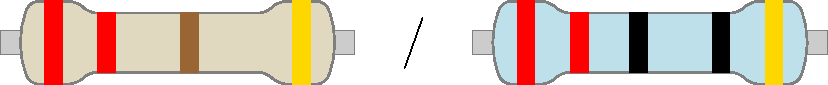
\includegraphics[width=0.5\textwidth]{kuvat/220.pdf}
\end{center}
\end{tcolorbox}

\begin{tcolorbox}[title=LEDin kytkeminen,colback=blue!10,colbacktitle=purple!90]\label{box:led}
Huomaa, että on merkitystä kummin päin LED kytketään koekytkentälevylle! 

LEDissä on kaksi jalkaa, joista toinen on pidempi. LEDin muovi on toiselta puolelta kaareva, ja toiselta siinä on suora leikkaus, lyhyempi jalka on suoran leikkauksen puolella. Lyhyemmän jalan nimi on katodi ja pidemmän jalan anodi.

\begin{minipage}{0.5\textwidth}
Piirrosmerkissä:
\begin{center}
\begin{tikzpicture}
%\node at (-1,0) {anodi};
\draw (0,0) node[left,text width=1.5cm] {anodi\\ pitkä jalka} to[led,o-o] (2,0) node[right,text width=2cm] {katodi\\lyhyt jalka};
\end{tikzpicture}
\end{center}
\end{minipage}
\begin{minipage}{0.5\textwidth}
\begin{tikzpicture}
\node (led) at (0,0) {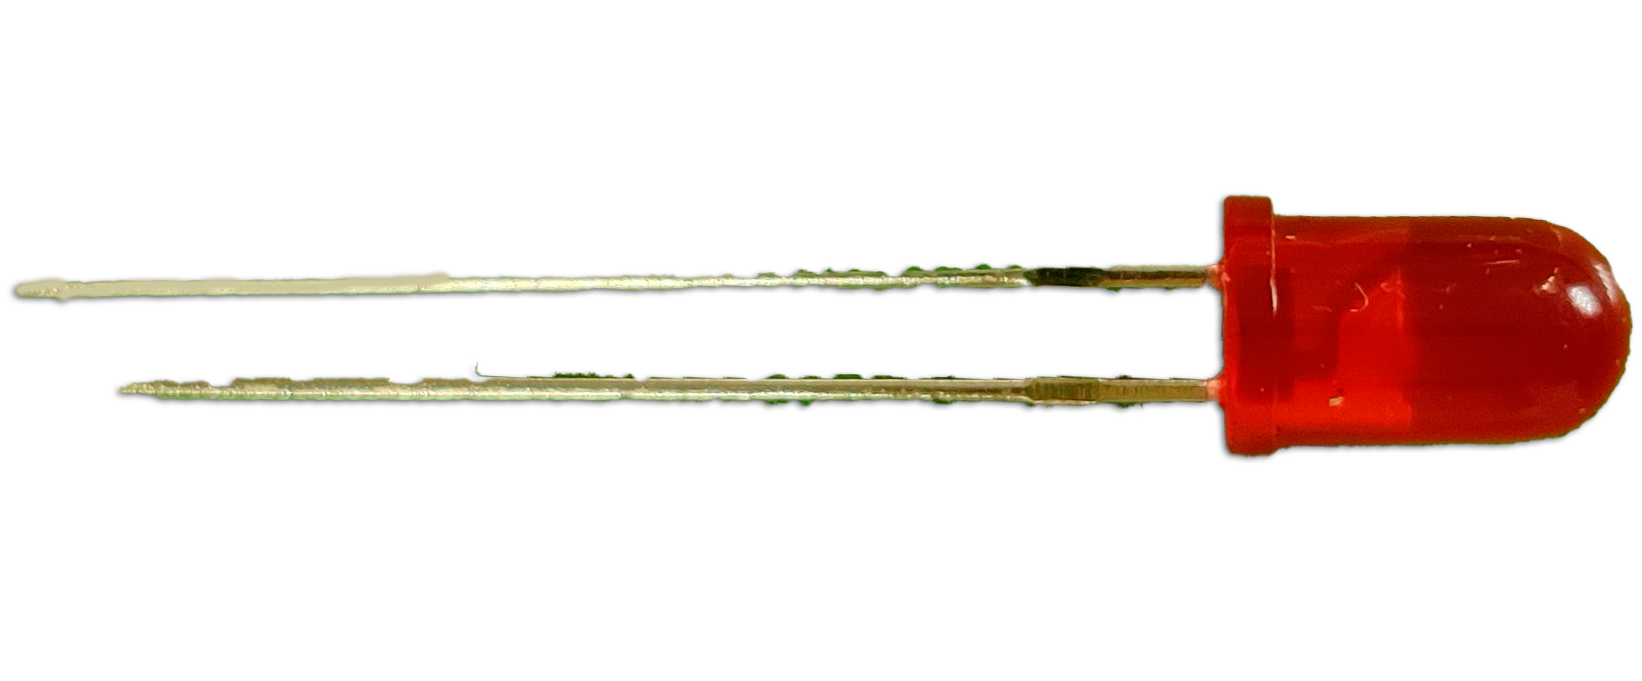
\includegraphics[width=0.95\textwidth]{kuvat/led.png}};
\node[above=0.5] (led) {Anodi (pitkä jalka)};
\node[below=0.5] (led) {Katodi (lyhyt jalka) + tasainen puoli};
\end{tikzpicture}
\end{minipage}

LED, eli valoa säteilevä diodi päästää virtaa läpi vain toiseen suuntaan kuten diodit. Jos anodille kytketään tarpeeksi suuri jännite verrattuna katodiin, virta kulkee ja valo palaa. Jos taas katodilla on suurempi jännite kuin anodilla, virtaa ei kulje ja LED ei pala. Jos anodilla ei ole tarpeeksi suuri jännite verrattuna katodiin, virta ei kulje. Riippuen LEDistä, vaadittu kynnysjännite voi vaihdella ja on tyypillisesti 1,5-4,5 volttia. 
\end{tcolorbox}

\begin{tcolorbox}[title=Jännitelähteen kytkeminen]
Jännitelähde on Arduinossa sisäänrakennettuna. Jotta voimme kytkeä jännitelähteen piiriin, tarvitsemme jännitelähteen molemmat päät: +5V ja maan (GND), kytkemällä vain toinen piiriin emme saa aikaan haluttua vaikutusta.

Arduino levyllä on kolme eri GND-riviä, ja mikä tahansa niistä käy. Kuvassa selvyyden vuoksi ne on numeroitu.

\begin{minipage}{0.3\textwidth}
\begin{tikzpicture}
\ctikzset{american}
\draw (-2,0.5) node[above] {5V} to[short,o-]  (-2,0) to[V,l=$5V$] (-2,-2) to[short,-o] (-2,-2.5) node[below] {GND};
%\node (-2,0.5) {5V};
\end{tikzpicture}
 \end{minipage}
\begin{minipage}{0.7\textwidth}
\begin{tikzpicture}[scale=0.5]
\pic[scale=0.2] at (0,0) {myarduino};
\draw[red,wire] (Ar5V) to[short,*-o] ++(-5,0) node[left,black] {5V};
\draw[black,wire] (ArGND2) to[short,*-o] ++(-5,0) node[left,black] {GND};
\end{tikzpicture}
\end{minipage}
\end{tcolorbox}

\begin{tcolorbox}[title=Painonapin kytkeminen,colback=blue!10,colbacktitle=purple!90]
Arduinon mukana tulevassa painonapissa on neljä pinniä, ja asetetaan keskellä olevan uran ylitse. Jos nappia ei paineta, niin A-E ja F-J rivillä 2 ovat samaa pistettä, mutta eri pistettä kuin rivin 4 (A-E) ja (F-J). Jos nappia painetaan, niin molempien rivien (2 ja 4) kaikki pisteet ovat kiinni toisissaan.


\begin{tikzpicture}[scale=0.5]
\BREADBOARD (0,0) {5};
\draw[thick,fill=hopea] (E2.east) rectangle (F4.west) coordinate[pos=0.5] (Y);
\draw[fill=black] (Y) circle (0.5);
\draw (E2.east) to[short,*-*] (E2);
\draw (E4.east) to[short,*-*] (E4);
\draw (F4.west) to[short,*-*] (F4);
\draw (F2.west) to[short,*-*] (F2);
\end{tikzpicture}
\end{tcolorbox}

\begin{tcolorbox}[title=Lämpötila-anturi,colback=blue!10,colbacktitle=purple!90]
Huomaa, että on merkitystä miten päin lämpötila-anturi kytketään piiriin! 

Jos tasainen sivu on kohti sinua, silloin vasemman puoleisin jalka on käyttöjännite (5V), keskimmäiseltä jalalta (A niin kuin anturi) voidaan lukea tulos ja oikean puoleisin jalka kytketään maahan (GND).

\begin{center}
\begin{tikzpicture}
\node[draw, minimum height=2,color=white,fill=black] (A) at (0,0) {TMP};
\draw[fill=black] (A.north west) to[bend left=70] (A.north east);
\draw[thick] (A.south west)++(0.1,0) --++(0,-0.5) to[short] ++(0,-.5) node[below,left] {5V};
\draw[thick] (A.south) --++(0,-0.5) to[short] ++(0,-.5) node[below] {A};
\draw[thick] (A.south east)++(-0.1,0) --++(0,-0.5) to[short] ++(0,-.5) node[below,right] {GND};
\end{tikzpicture}
\end{center}

Jos kytket anturin väärinpäin, se voi kuumentua. Ole siis tarkkana!
\end{tcolorbox}

\begin{tcolorbox}[title=Valoanturin kytkeminen,colback=blue!10,colbacktitle=purple!90]
Huomaa, että on merkitystä kummin päin valoanturi kytketään koekytkentälevylle! 

Valoanturissa on kaksi jalkaa, joista toinen on pidempi. Valodiodi näyttää kirkkaalta LEDiltä, mutta siitä puuttuu pyöristetty yläosa, eli yläpinta on tasainen (toisin kuin LEDeillä, joilla se on pyöreä). Piirrosmerkissä nuolet tulevat kohti diodia, eli olemme ottamassa valoa sisään (emmekä lähettämässä sitä ulos kuten LEDin kanssa). 

Valoanturin muovi on toiselta puolelta kaareva, ja toiselta siinä on suora leikkaus, lyhyempi jalka on suoran leikkauksen puolella. Lyhyemmän jalan nimi on katodi ja pidemmän jalan anodi.

Piirrosmerkissä:
\begin{center}
\begin{tikzpicture}
%\node at (-1,0) {anodi};
\draw (0,0) node[left,text width=1.5cm] {anodi\\ pitkä jalka} to[photodiode,o-o] (2,0) node[right,text width=2cm] {katodi\\lyhyt jalka};
\end{tikzpicture}
\end{center}

Valodiodi kytketään myös aina vastuksen kanssa sarjaan, nyt käytössä on 10k$\Omega$ vastus. 
\end{tcolorbox}

\begin{tcolorbox}[title=Potentiometrin kytkeminen,colback=blue!10,colbacktitle=purple!90]
Potentiometri on säädettävä vastus, jossa on kolme jalkaa, kaksi toisella puolella ja yksi toisella. Se kytketään uran ylitse, niin että kaksi jaloista ovat toisella puolella ja yksi toisella puolella. Potentiometrin mukana tulee valkoinen säätönuppi, jolla vastuksen arvoa voidaan säädellä pyörittämällä nuppia. 

\begin{minipage}{0.8\textwidth}
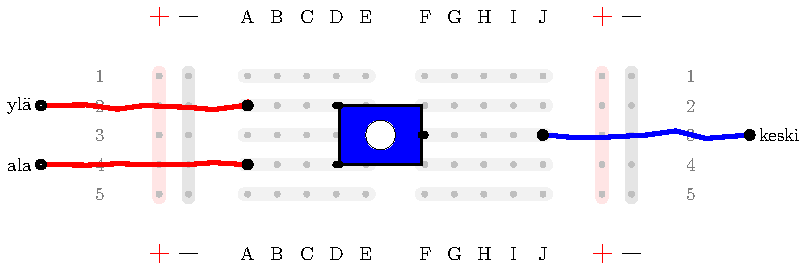
\includegraphics[width=\textwidth]{kuvat/kuva17.pdf}
\end{minipage}%
\begin{minipage}{0.2\textwidth}
Piirrustusmerkki:

\begin{circuitikz} 
\draw (0,0) node[left] {ylä} to[american potentiometer,n=mypot] ++(0,-2) node[right] {ala} (mypot.wiper) to[short] ++(1,0) node[above] {keski};
\end{circuitikz}
\end{minipage}

Mitattaessa vastuksen arvoa välillä ylä-ala, vastuksen arvo pysyy vakiona. Jos taas käytetään vastusta välillä ylä-keski tai keski-ala, vastuksen arvoa voidaan muuttaa pyörittämällä säätönuppia.
\end{tcolorbox}

\begin{tcolorbox}[title=Kaltevuusanturin kytkeminen,colback=blue!10,colbacktitle=purple!90]
Kaltevuusanturissa on neljä jalkaa, ja se vaatii kaksi riviä koekytkentälevystä. Kaltevuusanturi näyttää suorakulmaiselta laatikolta, jonka lähes neliönmuotoisella päällä lukee "UP" ja on nuoli ylös. Tämä rivi, jolla nuoli on, kytketään käyttöjänniteeseen ja toinen rivi kytketään vastuksen kautta maahan. Mittaustulos voidaan lukea samalta riviltä mille vastus on kytketty.  


\begin{tikzpicture}[scale=0.5]
\BREADBOARD (0,0) {5};
\draw[thick,fill=black] (D3.east) rectangle (E4.west) node[pos=0.5,color=white] {UP};
\draw (D3.east) to[short,*-*] (D3);
\draw (D4.east) to[short,*-*] (D4);
\draw (E3.west) to[short,*-*] (E3);
\draw (E4.west) to[short,*-*] (E4);

\draw[wire,red] (A3) to[short,*-o] ++(-7,0) node[left,black] {Käyttöjännite};
\draw[wire,blue] (A4) to[short,*-o] ++(-7,0) node[left,black] {Mittaus};

\end{tikzpicture}
\end{tcolorbox}

\begin{tcolorbox}[title=LCD-näyttö,colback=blue!10,colbacktitle=purple!90]
Tämä on tarkemmin esitelty kappaleessa \ref{sec:lcd} ja tarkemmin kuvassa sivulla \pageref{fig:lcd}. Tällöin LCD-näyttöä ohjataan seuraavilla komennoilla.

\begin{lstlisting}[numbers=none]
#include <LiquidCrystal.h> // Lisataan kirjasto 
LiquidCrystal lcd(13,11,5,4,3,2); // Digital Pinnit joissa kiinni

void setup() {
  lcd.begin(16,2); // Kaynnistetaan naytto
  lcd.print("Tervetuloa"); // Kirjoitetaan ekalle riville
}

void loop() {
  lcd.setCursor(0,1); // Siirrytaan toiselle riville
  lcd.print("Nimi"); // Kirjoita oma nimesi tahan
}
\end{lstlisting}


\end{tcolorbox}
\chapter{Vinkit Arduinolla koodaamiseen}
Tässä osuudessa on koottu yhteen kaikki vinkit paketin osalta.

\begin{tcolorbox}[colback=white,title=Vinkkejä Arduinolla koodaamiseen!,colbacktitle=purple!90, breakable]
Seuraavassa esitellään Arduinolla koodaamiseen liittyviä vinkkejä. 
\begin{lstlisting}
// Kaksi kauttaviivaa aloittaa kommentin. Tata ei siis lueta koodissa vaan on tiedoksi koodin lukijalle

pinMode(luku, tyyppi) // Talla voit saataa pinnien 0-13 tekoa laittamalla sanan luku tilalle luvun jolta rivilta haluat komentaa
// Tyypin tilalle voit kirjoittaa joko OUTPUT eli Arduino lahettaa signaalia
// tai INPUT jolloin Arduino vastaanottaa signaalin

digitalWrite(luku, arvo) // Talla voit muuttaa pinniin luku kirjoitettua arvoa
// arvo HIGH vastaa 5V jannitetta
// arvo LOW vastaa 0V jannitetta

delay(luku) // Odottaa luvun verran millisekunteja
\end{lstlisting}
\end{tcolorbox}

\begin{tcolorbox}[colback=white,title=Vinkkejä Arduinolla koodaamiseen!,colbacktitle=purple!90, breakable]
\begin{lstlisting}
muuttuja = digitalRead(luku); // Lukee pinnin luku arvon ja tallentaa sen muuttujaan muuttuja
// Huomaa etta muuttujalla pitaa olla annettuna tyyppi
// Esimerkiksi bool:
bool muuttuja = digitalRead(luku); 
// bool voi olla joko HIGH tai LOW sen mukaan mita tassa tapauksessa luettiin piirista
// bool on kateva tilanteissa joissa arvo on joko HIGH tai LOW

// Ehtorakenne
// Tarkastetaan muuttujan arvo.
if (muuttuja == HIGH) {
   // jos muuttujan arvo on HIGH tehdaan koodi tassa valissa
} else {
   // muuten (eli kun LOW) tehdaan mita tassa kirjoitetaan
}
\end{lstlisting}
\end{tcolorbox}

\begin{tcolorbox}[colback=white,title=Vinkkejä Arduinolla koodaamiseen!,colbacktitle=purple!90, breakable]
\begin{lstlisting}
bool ledStatus = true; // Luodaan muuttuja, jonka arvo on totta

ledStatus = !ledStatus; // Muuttaa muuttujan ledStatus arvoksi arvon epatosi (jos arvo oli tosi) tai tosi (jos arvo oli epatosi)
\end{lstlisting}
\end{tcolorbox}

\begin{tcolorbox}[colback=white,title=Vinkkejä Arduinolla koodaamiseen!,colbacktitle=purple!90, breakable]
\begin{lstlisting}
// Seuraava rivi lisataan setup() funktioon
attachInterrupt(digitalPinToInterrupt(luku), keskeytys, FALLING);
// attachInterrupt on komento jolla luodaan keskeytys
// digitalPinToInterrupt(luku) kertoo mista pinnista saadaan painallus
// keskeytys on aliohjelmanne nimi, johon siirrytaan
// FALLING on parametri joka tarkoittaa kun nappia painetaan alas
// Vaihtoehtona ovat myos
// LOW kun pinnin luku jannite on 0V
// CHANGE kun pinnin luku jannite muuttuu
// RISING kun pinnin tila muuttuu nollasta viiteen volttiin
// FALLING kun pinnin tila muuttuu viidesta voltista nollaan

// Maaritetaan uusi funktio olemassa olevien peraan
void keskeytys() {
  // Mita funktio tekee?
  // Esimerkiksi vaihtaa muuttujan ledState arvo:
  ledState = !ledState;
}
// Talloin ohjelman alussa pitaa olla maaritys
volative bool ledState = false;
// volative tarkoittaa, etta muuttujan arvo tarkastetaan aina sita kaytettaessa
// muuttujan ledState arvo voi siis muuttua milloin vain ohjelman aikana
\end{lstlisting}
\end{tcolorbox}

\begin{tcolorbox}[colback=white,title=Vinkkejä Arduinolla koodaamiseen!,colbacktitle=purple!90, breakable]
\begin{lstlisting}
// Seuraava rivi kuuluu setup()-funktion sisalle
Serial.begin(9600); // Aloittaa kommunnikoinnin tietokoneen kanssa
// 9600 kertoo kuinka monta bittia sekunnissa lahetetaan.

// Komentoja, joilla voidaan tulostaa
Serial.print(muuttuja); // Tulostetaan muuttujan muuttuja arvo
Serial.print("Teksti:"); // Tulostetaan Teksti: 
Serial.println(muuttuja); // Sama kuin muuttujan tulostus, mutta rivinvaihto lopussa
Serial.print("\n"); // Rivinvaihto manuaalisesti
\end{lstlisting}
\end{tcolorbox}

\begin{tcolorbox}[colback=white,title=Vinkkejä Arduinolla koodaamiseen!,colbacktitle=purple!90, breakable]
\begin{lstlisting}
// Halutaan tehda monta asiaa riippuen monesta asiasta
if (ehto) {
    // Mita tehdaan jos ehto patee
} else if (ehto2) {
    // Mita tehdaan jos ehto2 patee
} else if (ehto3) {
   // Naita voit lisata niin monta kuin tarvitset
} else {
    // Ja halutessa voit maaritella myos mita tehdaan muulloin
}

// Erilaisia ehtoja
muuttuja < luku // Muuttujan muuttuja arvo on pienempi kuin annettu luku
muuttuja <= luku // Muuttujan muuttuja arvo on pienempi tai yhta suuri kuin luku
muuttuja > luku // Muuttuja on suurempi kuin luku
// Kaksi ehtoa yhta aikaa
muuttuja >= luku1 && muuttuja < luku2 // Muuttuja on suurempi tai yhtasuuri kuin luku1 JA pienempi kuin luku2
\end{lstlisting}
\end{tcolorbox}

\begin{tcolorbox}[colback=white,title=Vinkkejä Arduinolla koodaamiseen!,colbacktitle=purple!90, breakable]
\begin{lstlisting}
// Satunnaisen luvun arpominen
int satunnainen = random(luku); //  satunnainen kokonaisluku valilta 0-annettu luku
// Ehtolause: ei yhta suuri kuin
luku1 != luku2
// Vaihtoehtoisia tapauksia
switch(luku) {
    case 0:
    // mita tehdaan jos luku on nolla
    break; // lopetetaan
    case 1: 
    // kun luku on 1
    break;
    // Lisaa case numero: riveja niin monta yhteensa kuin lukusi on ja kerro mita tehdaan, ja poistu sen jalkeen ulompaan koodiin break:n avulla
}
\end{lstlisting}
\end{tcolorbox}

\begin{tcolorbox}[colback=white,title=Vinkkejä Arduinolla koodaamiseen!,colbacktitle=purple!90, breakable]
\begin{lstlisting}
// Satunnaisen luvun arpominen
int satunnainen = random(luku); //  satunnainen kokonaisluku valilta 0-annettu luku
// Ehtolause: ei yhta suuri kuin
luku1 != luku2
// Vaihtoehtoisia tapauksia
switch(luku) {
    case 0:
    // mita tehdaan jos luku on nolla
    break; // lopetetaan
    case 1: 
    // kun luku on 1
    break;
    // Lisaa case numero: riveja niin monta yhteensa kuin lukusi on ja kerro mita tehdaan, ja poistu sen jalkeen ulompaan koodiin break:n avulla
}
\end{lstlisting}
\end{tcolorbox}
\chapter{Vastusten värikoodit}\label{varikoodit}
Arduinon mukana tulevissa vastuksissa on käytössä joko kahdenlaisia vastusmerkintöjä, joko neljällä tai viidellä viivalla.

Näistä viimeinen kertoo kuinka tarkasti vastuksen arvo osuu annettuun arvoon, ja nämä viivat ovat usien kultaisia tai hopeisia. Tämän avulla voit yrittää tunnistaa kummasta päästä vastuksen arvoa ollaan lukemassa. 

Kaksi tai kolme ensimmäistä viivaa kuvaa vastuksen numeroarvoa ja kolmas tai neljäs viiva kuvaa vastuksen kokoluokkaa (eli kerrointa, esimerkiksi $k=1000$). 

%%%%%%%%%%%%%%%%%%%%%%%%%%%%%%%%
\definecolor{rbrown}{HTML}{996633}
\definecolor{rred}{HTML}{FF0000}
\definecolor{rorange}{HTML}{FF9900}
\definecolor{ryellow}{HTML}{FFFF00}
\definecolor{rgreen}{HTML}{228b22}
\definecolor{rblue}{HTML}{0047AB}
\definecolor{rviolet}{HTML}{800080}
\definecolor{rgrey}{HTML}{CCCCCC}
\definecolor{rwhite}{HTML}{FFFFFF}
\definecolor{kulta}{HTML}{FFD700}
\definecolor{hopea}{HTML}{C0C0C0}
%%%%%%%%%%%%%%%%%%%%%%%%%%%%%%%
\begin{minipage}{0.4\textwidth}
Kahden tai kolmen ensimmäisen viivan värit ja niitä vastaavat numerot:

\begin{tikzpicture}
  \draw[fill=black] (0,0) rectangle ++(2,1) node[pos=(0.5),white] {0};
  \draw[fill=rbrown] (0,-1) rectangle ++(2,1) node[pos=0.5,white] {1};
    \draw[fill=rred] (0,-2) rectangle ++(2,1) node[pos=(0.5),white] {2};
  \draw[fill=rorange] (0,-3) rectangle ++(2,1) node[pos=0.5,white] {3};
    \draw[fill=ryellow] (0,-4) rectangle ++(2,1) node[pos=(0.5),white] {4};
  \draw[fill=rgreen] (0,-5) rectangle ++(2,1) node[pos=0.5,white] {5};
    \draw[fill=rblue] (0,-6) rectangle ++(2,1) node[pos=(0.5),white] {6};
  \draw[fill=rviolet] (0,-7) rectangle ++(2,1) node[pos=0.5,white] {7};
  \draw[fill=rgrey] (0,-8) rectangle ++(2,1) node[pos=(0.5),white] {0};
  \draw[fill=rwhite] (0,-9) rectangle ++(2,1) node[pos=0.5,black] {9};
  %\draw[draw=black] (11.1,5.5) rectangle ++(0.3,0.3);
\end{tikzpicture}
\end{minipage}
\begin{minipage}{0.3\textwidth}
Kertoimen suuruus, $10^{x}$, missä $x$ on listassa annettu luku:

\begin{tikzpicture}
  \draw[fill=black] (0,0) rectangle ++(2,1) node[pos=(0.5),white] {0};
  \draw[fill=rbrown] (0,-1) rectangle ++(2,1) node[pos=0.5,white] {1};
    \draw[fill=rred] (0,-2) rectangle ++(2,1) node[pos=(0.5),white] {2};
  \draw[fill=rorange] (0,-3) rectangle ++(2,1) node[pos=0.5,white] {3};
    \draw[fill=ryellow] (0,-4) rectangle ++(2,1) node[pos=(0.5),white] {4};
  \draw[fill=rgreen] (0,-5) rectangle ++(2,1) node[pos=0.5,white] {5};
    \draw[fill=rblue] (0,-6) rectangle ++(2,1) node[pos=(0.5),white] {6};
\end{tikzpicture}
\end{minipage}
\begin{minipage}{0.2\textwidth}
Toleranssin\\ suuruus:

\begin{tikzpicture}
  \draw[fill=rbrown] (0,-1) rectangle ++(2,1) node[pos=0.5,white] {$\pm1\%$};
    \draw[fill=rred] (0,-2) rectangle ++(2,1) node[pos=(0.5),white] {$\pm2\%$};
  \draw[fill=kulta] (0,-3) rectangle ++(2,1) node[pos=0.5,white] {$\pm5\%$ kulta};
    \draw[fill=hopea] (0,-4) rectangle ++(2,1) node[pos=(0.5),white] {$\pm10\%$ hopea};
\end{tikzpicture}
\end{minipage}


\begin{table}[!h]
\caption {Paketissa mukana olevat vastukset.} \label{tab:varikooditv} 
\begin{center}
\begin{tabular}{c|c}
    Vastus & Kuvat  \\\hline\\
   $220\Omega$  & 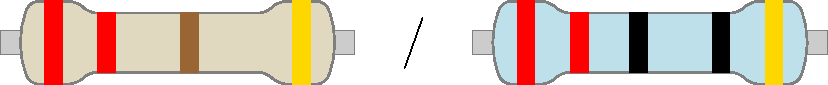
\includegraphics[width=0.5\textwidth]{kuvat/220.pdf} \\\hline\\
   $560\Omega$  & 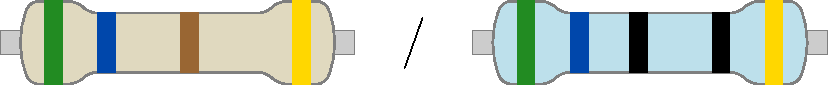
\includegraphics[width=0.5\textwidth]{kuvat/560.pdf} \\\hline\\
   $1\text{k}\Omega$  & 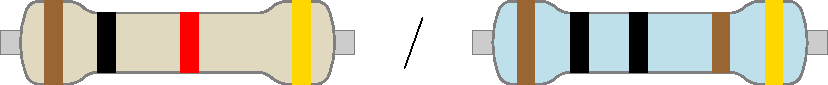
\includegraphics[width=0.5\textwidth]{kuvat/1k.pdf} \\\hline\\
   $4.7\text{k}\Omega$  & 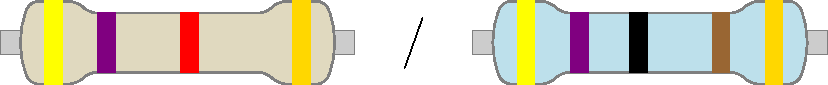
\includegraphics[width=0.5\textwidth]{kuvat/4k7.pdf} \\\hline\\
   $10\text{k}\Omega$  & \includegraphics[width=0.5\textwidth]{kuvat/10k.pdf} \\\hline\\
$1\text{M}\Omega$  & \includegraphics[width=0.5\textwidth]{kuvat/1M.pdf} \\\hline\\
   $10\text{M}\Omega$  & \includegraphics[width=0.5\textwidth]{kuvat/10M.pdf} \\\hline
\end{tabular}
\end{center}
\end{table}

\begin{tcolorbox}[colback=red!10,colbacktitle=red,title=HUOM!]
Jos käytössäsi on yleismittari, voit tarkistaa vastuksen arvon sillä!
\end{tcolorbox}





\clearpage
\pagestyle{plain}
\pagenumbering{gobble}
\begin{huge}
Arduino-paketti yläkouluun ja lukioon
\end{huge}


\begin{itemize}
    \item Koekytkentälevy
    \item LED
    \item Liikennevalot
    \item Lämpö- ja valoanturit
    \item LCD-näyttö
    \item Kaltevuusanturi
\end{itemize}

\includegraphics[width=\textwidth]{kuvat/kansikuva_taka2022.jpg}


\end{document}
